\documentclass[10pt, a4paper]{article}
\usepackage{preamble}
\usepackage{tikz-cd}

\newcommand{\ts}[1]{\textsuperscript{#1}}

\title{Linear Algebra I}
\author{Luke Phillips}
\date{October 2024}

\begin{document}

\maketitle

\newpage

\tableofcontents

\newpage

\section{Vectors and vector spaces}

\subsection{Vector space \texorpdfstring{$\R ^ n$}{}}

\begin{definition}
    $n$-dimensional real space $\R ^ n$ a set of elements as such\[
    \R ^ n = \left\{\underline{x} = \begin{pmatrix}
        x_1 \\
        x_2 \\
        \vdots \\
        x_n
    \end{pmatrix}
    \quad:\ x_i \in \R
    \right\}\footnote{Vectors are $\underline{x}$ or $\mbf{x}$.}\]
\end{definition}

\begin{definition}
    The zero vector is defined as
    \[
    \mbf{0} = \begin{pmatrix}
        0 \\
        0 \\
        \vdots \\
        0
    \end{pmatrix}
    \in \R ^ n
    \]
\end{definition}

There are two operations on $\R ^ n$

\textbf{Vector addition}:

Vector addition is a function defined as such
\[
\R ^ n \times \R ^ n \mapsto \R ^ n
\]
This function takes two vectors $\mbf{v, w}$ and obtains
\[
(\mbf{v, w})\mapsto \mbf{v + w}
\]
For example
\[
\mbf{v + w} = \begin{pmatrix}
    v_1 \\
    v_2 \\
    \vdots \\
    v_n
\end{pmatrix} + \begin{pmatrix}
    w_1 \\
    w_2 \\
    \vdots \\
    w_n
\end{pmatrix}
=
\begin{pmatrix}
    v_1 + w_1 \\
    v_2 + w_2 \\
    \vdots \\
    v_n + w_n
\end{pmatrix}
=
\mbf{v + w}
\]

\textbf{Scalar multiplication}:

Scalar multiplication is defined as a function
\[
\R \times \R ^ n \mapsto \R ^ n.
\]
This is written as follows
\[
(\lambda, \mbf{v}) \mapsto \lambda\mbf{v}
\]
The operation is defined as such
\[
\lambda\mbf{v} = \lambda\begin{pmatrix}
    v_1 \\
    v_2 \\
    \vdots \\
    v_n
\end{pmatrix}
=
\begin{pmatrix}
    \lambda v_1 \\
    \lambda v_2 \\
    \vdots \\
    \lambda v_n
\end{pmatrix}
\]

\textbf{Intuition}

Vectors can be thought of a point in $n$-dimensional space
\begin{figure}[H]
    \centering
    \begin{tikzpicture}
    \draw[->] (0,0) -- (0,2);
    \draw[->] (0,0) -- (2,0);
    \draw[->] (0,0) -- (1.5,1);
    \filldraw (1,1) circle (2pt);
    \end{tikzpicture}
    \caption{Graph 1}
    \label{fig:Gr1}
\end{figure}

As a direction to a point
\begin{figure}[H]
    \centering
    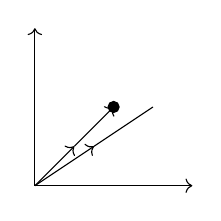
\begin{tikzpicture}
    \draw[->] (0,0) -- (0,2);
    \draw[->] (0,0) -- (2,0);
    \draw[->] (0,0) -- (0.75,0.5);
    \draw[-] (0.75,0.5) -- (1.5,1);
    \draw[->] (0,0) -- (0.5, 0.5);
    \draw[->] (0.5,0.5) -- (1, 1);
    \filldraw (1,1) circle (2pt);
    \end{tikzpicture}
    \caption{Graph 2}
    \label{fig:Gr2}
\end{figure}

As up to translation
\begin{figure}[H]
    \centering
    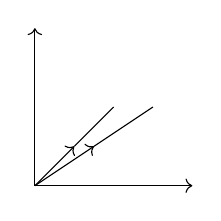
\begin{tikzpicture}
    \draw[->] (0,0) -- (0,2);
    \draw[->] (0,0) -- (2,0);
    \draw[->] (0,0) -- (0.75,0.5);
    \draw[-] (0.75,0.5) -- (1.5,1);
    \draw[->] (0,0) -- (0.5, 0.5);
    \draw[-] (0.5,0.5) -- (1, 1);
    \end{tikzpicture}
    \caption{Graph 3}
    \label{fig:Gr3}
\end{figure}

Vector addition
\begin{figure}[H]
    \centering
    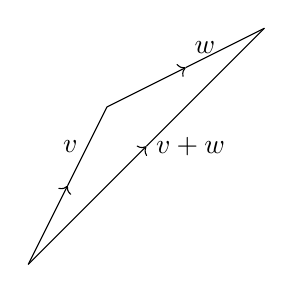
\begin{tikzpicture}
    \draw[->] (0,0) -- (0.5,1);
    \draw[-] (0.5,1) -- (1,2) node [midway, left] {$\mbf{v}$};
    \draw[->] (1,2) -- (2,2.5);
    \draw[-] (2,2.5) -- (3,3) node [midway, left] {$\mbf{w}$};
    \draw[->] (0,0) -- (1.5,1.5) node [right] {$\mbf{v + w}$};
    \draw[-] (1.5,1.5) -- (3,3);
    \end{tikzpicture}
    \caption{Graph 4}
    \label{fig:Gr4}
\end{figure}

Scalar multiplication
\begin{figure}[H]
    \centering
    \begin{tikzpicture}
    \draw[->] (2,2) -- (3,3) node[left] {$\mbf{v}$};
    \draw[-] (3,3) -- (4,4);
    \draw[->] (2,0) -- (4,2) node[left] {$\mbf{\lambda v}$};
    \draw[->] (4,2) -- (6,4);
    \end{tikzpicture}
    \caption{Graph 5}
    \label{fig:Gr5}
\end{figure}
\textbf{Gr5}


These operations satisfy the \textbf{axioms} of a real vector space.
\begin{enumerate}[label = (\roman*)]
    \item There exists an additive identity $\mbf{0} \in \R ^ n$ such that
    \[
    \mbf{0 + v = v + 0 = v} \ \forall \mbf{v} \in \R ^ n.
    \]
    \item Commutativity
    \[
    \forall\mbf{w, v} \in \R ^ n\quad\mbf{w + v =  v + w}
    \]
    \item Existence of additive inverses
    \[
    \forall\mbf{v} \in \R ^ n\ \exists\mbf{-v} \in \R ^ n \text{ s.t. } \mbf{v + (-v) = (-v) + v = 0}
    \]
    \item Associativity
    $\forall\mbf{u, v, w} \in \R ^ n$
    \[
    (\mbf{u + v}) + \mbf{w} = \mbf{u} + (\mbf{v + w})
    \]
\end{enumerate}
(i), (iii), (iv) $\iff (\R ^ n, +)$ is a group

(i), (ii), (iii), (iv) $\iff (\R ^ n, +)$ is an abelian group



\textbf{Axioms} for scalar multiplication
\begin{enumerate}[label = (\roman*)]
    \item $0\mbf{v} = \mbf{0}\quad\forall\mbf{v}\in \R ^ n$.
    \item $1\mbf{v} = \mbf{v}\quad\forall\mbf{v}\in \R ^ n$.
    \item Associativity
    \[
    \lambda (\mu\mbf{v}) = (\lambda\mu)\mbf{v}\quad\forall\lambda,\mu \in \R\quad\forall\mbf{v}\in\R ^ n
    \]
    \item Distributivity, $\forall\lambda,\mu\in\R\quad\forall\mbf{v, w} \in \R ^ n$
    \begin{align*}
    (\lambda + \mu)\mbf{v} &= \lambda\mbf{v} + \mu\mbf{v} \\
    \lambda(\mbf{v + w}) &= \lambda\mbf{v} + \lambda\mbf{w}
    \end{align*}
\end{enumerate}

$\R ^ n$ clearly satisfies these axioms (if not obvious check) because they can be checked component-wise once we set 
\[
-\mbf{v} = \begin{pmatrix}
    -v_1 \\
    -v_2 \\
    \vdots \\
    -v_n
\end{pmatrix}
\]

\begin{definition}
    Standard basis vectors
    
    For $1 \leq i \leq n$ we define $\mbf{e}_i \in \R ^ n$
    \[
    \mbf{e}_i = \begin{pmatrix}
        0 \\
        0 \\
        \vdots \\
        0 \\
        1\footnote{$i$th position from the top.} \\
        0 \\
        \vdots \\
        0
    \end{pmatrix}
    \]    
\end{definition}

\begin{example}
    \[
    \mbf{e}_1 = \begin{pmatrix}
        1 \\
        0 \\
        \vdots \\
        0
    \end{pmatrix}
    \]
    \[
    \mbf{e}_2 = \begin{pmatrix}
        0 \\
        1 \\
        \vdots \\
        0
    \end{pmatrix}
    \]
\end{example}

We can express any vector $\mbf{x} \in \R ^ n$ uniquely as a linear combination of the standard basis vectors.

\begin{example}
    \begin{align*}
    \mbf{x} &= \begin{pmatrix}
        x_1 \\
        x_2 \\
        \vdots \\
        x_n
    \end{pmatrix}
    =
    x_1 \begin{pmatrix}
        1 \\
        0 \\
        \vdots \\
        0
    \end{pmatrix}
    +
    x_2 \begin{pmatrix}
        0 \\
        1 \\
        \vdots \\
        0
    \end{pmatrix}
    +
    \dots
    +
    x_n \begin{pmatrix}
        0 \\
        0 \\
        \vdots \\
        0 \\
        1
    \end{pmatrix} \\
    &= x_1 \mbf{e}_1 + x_2 \mbf{e}_2 + \dots + x_n \mbf{e}_n
    \end{align*}
\end{example}
The $x_i$'s are sometimes called the Cartesian coordinates of the vector $\mbf{x}$.

\subsection{The scalar (or dot) product in \texorpdfstring{$\R ^ n$}{}}

\begin{definition}
    The scalar product is defined as $\R ^ n \times \R ^ n \mapsto \R$, $(\mbf{u, v}) \mapsto \mbf{u \cdot v}$
    \begin{align*}
    \mbf{u \cdot v} &= \begin{pmatrix}
        u_1 \\
        u_2 \\
        \vdots \\
        u_n
    \end{pmatrix} \cdot
    \begin{pmatrix}
        v_1 \\
        v_2 \\
        \vdots \\
        v_n
    \end{pmatrix} \\
    &= u_1 v_1 + u_2 v_2 + \dots + u_n v_n  \\
    &= \sum_{i = 1}^{n}u_iv_i \in \R
    \end{align*}
\end{definition}

\begin{example}
    \[
    \begin{pmatrix}
        4 \\
        1 \\
        2
    \end{pmatrix}
    \cdot
    \begin{pmatrix}
        -3 \\
        -2 \\
        1
    \end{pmatrix}
    =
    -12 - 2 + 2 = -12.
    \]
\end{example}


\textbf{Axioms} of the scalar product
% To-Do add in the foralls here
\begin{enumerate}[label = (\roman*)]
    \item Symmetry
    \[
    \mbf{u \cdot v = v \cdot u}\qquad\forall\mbf{u, v} \in \R ^ n
    \]
    \item Linearity (1)
    \begin{align*}
    (\mbf{u + v)\cdot w}) &= \mbf{u \cdot w + v \cdot w}\qquad\forall \lambda \in \R\\
    \lambda\mbf{u})\cdot \mbf{w} &= \lambda (\mbf{u \cdot w})\qquad\forall\mbf{u, v, w} \in \R ^ n
    \end{align*}
    \item Linearity (2)
    \begin{align*}
        \mbf{u} \cdot (\mbf{v + w}) &= \mbf{u} \cdot \mbf{v} + \mbf{u} \cdot \mbf{w}\qquad \forall \lambda \in \R \\
        \mbf{u} \cdot \lambda\mbf{v} &= \lambda(\mbf{u \cdot v})\qquad \forall\mbf{u, v, w} \in \R ^ n
    \end{align*}
    \item Positivity
    \begin{align*}
        \mbf{v \cdot v} \geq 0\quad \forall \mbf{v} \in \R ^ n \\
        \text{and } \mbf{v \cdot v} = 0 \iff \mbf{v = 0}
    \end{align*}
\end{enumerate}

\begin{definition}
    Given a vector $\mbf{v} \in \R ^ n$ we define its magnitude (or length) to be
    \[
    |\mbf{v}| = \sqrt{\mbf{v \cdot v}}
    \]
\end{definition}
Note $\mbf{v \cdot v} \geq 0$ so positive square roots exist. Likewise note

$|\mbf{v}| \geq 0 \text{ and } |\mbf{v}| = 0 \iff \mbf{v = 0}$

\begin{example}
    \[
    \left|\begin{pmatrix}
        -3 \\
        4
    \end{pmatrix}\right|
    = \sqrt{(-3) ^ 2 + 4 ^ 2} = \sqrt{25} = 5
    \]
\end{example}

Thinking about a vector $\mbf{v} \in \R ^ 2$ where $\mbf{v \neq 0}$
\begin{figure}[H]
    \centering
    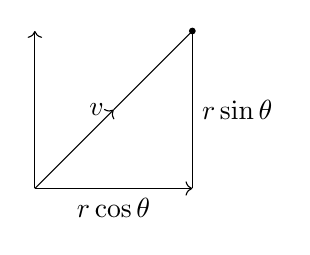
\begin{tikzpicture}
    \draw[->] (0,0) -- (0,2);
    \draw[->] (0,0) -- (2,0);
    \draw[->] (0,0) -- (1,1) node[left] {$\mbf{v}$};
    \draw[-] (1,1) -- (2,2);
    \draw[-] (2,0) -- (2,2) node[midway, right] {$r\sin\theta$};
    \draw[-] (0,0) -- (2,0) node[midway, below] {$r\cos\theta$};
    \filldraw (2,2) circle (1pt);
    \end{tikzpicture}
    \caption{Graph 9}
    \label{fig:Gr9}
\end{figure}

\[
\mbf{v}  = \begin{pmatrix}
    r\cos\theta \\
    r\sin\theta
\end{pmatrix}
\]
where
$r = |\mbf{v}|$ and $0 \leq \theta < 2\pi$, $\theta$ is the angle made by $\mbf{v}$ in an anticlockwise direction with the positive real axis.

We define $(r, \theta) \in (0, \infty) \times [0, 2\pi)$
to be the unique numbers such that
$\mbf{v}  = \begin{pmatrix}
    r\cos\theta \\
    r\sin\theta
\end{pmatrix}$
we call $(r, \theta)$ the polar coordinates of $\mbf{v}$

\begin{example}
    Suppose $\mbf{v} = \begin{pmatrix}
        2 \\
        3
    \end{pmatrix}$,
    what are its polar coordinates?

    $r = |\mbf{v}| = \sqrt{2 ^ 2 + 3 ^ 2} = \sqrt{13}$

    $\theta = \arcsin \left({\dfrac{3}{\sqrt{13}}}\right)$
\end{example}

\begin{example}
    Suppose $\mbf{v} = \begin{pmatrix}
        2 \\
        -2
    \end{pmatrix}$,
    what are its polar coordinates?

    $r = |\mbf{v}| = \sqrt{2 ^ 2 + (-2) ^ 2} = \sqrt{8} = 2\sqrt{2}$

    $\theta = \dfrac{7\pi}{4}$
\end{example}

\begin{proposition}
    Suppose $\mbf{v}, \mbf{w} \in \R ^ n$
    \[
    |\mbf{v}| = r,\quad|\mbf{w}| = s
    \]
    Suppose that $\mbf{v}, \mbf{w}$ make an angle of $\alpha$ with each other $0 \leq \alpha \leq \pi$
    
    Then $\mbf{v}\cdot\mbf{w} = rs\cos(\alpha)$.
    \begin{proof}
        Suppose polar coordinated of $\mbf{v}$ are $(r, \theta)$, and of $\mbf{w}$ are $(s, \varphi)$.

        Then $\mbf{v} = \begin{pmatrix}
            r\cos\theta \\
            r\sin\theta
        \end{pmatrix}$, $\mbf{w} = \begin{pmatrix}
            s\cos\varphi \\
            s\sin\varphi
        \end{pmatrix}$
        \begin{align*}
        \mbf{v\cdot w} &= \begin{pmatrix}
            r\cos\theta \\
            r\sin\theta
        \end{pmatrix} \cdot \begin{pmatrix}
            s\cos\varphi \\
            s\sin\varphi
        \end{pmatrix} \\
        &= rs\cos\theta\cos\varphi + rs\sin\theta\sin\varphi \\
        &= rs(\cos\theta\cos\varphi + \sin\theta\sin\varphi) \\
        &= rs(\cos(\theta - \varphi) \\
        &= rs\cos(\pm\alpha) = rs\cos\alpha.
        \end{align*}
    \end{proof}
\end{proposition}

\begin{corollary}
    If $\mbf{v} \neq \mbf{0}$ and $\mbf{w} \neq \mbf{0}$.
    $\mbf{v}$ and $\mbf{w}$ are orthogonal if and only if
    \[
    \mbf{v \cdot w} = 0.
    \]
    \begin{proof}
        \[
        \mbf{v \cdot w} = 0 \iff \cos(\alpha) = 0 \iff \alpha = \frac{\pi}{2}
        \]
    \end{proof}
\end{corollary}

\begin{example}
    $\mbf{v} = \begin{pmatrix}
        6 \\
        -2
    \end{pmatrix}\qquad
    \mbf{w} = \begin{pmatrix}
        -1 \\
        -3
    \end{pmatrix}$

    Then $\mbf{v\cdot w} = 6(-1) + (-2)(-3) = 0$

    So $\mbf{v, w}$ are orthogonal.
\end{example}


\begin{theorem}[Cauchy-Schwarz inequality]
    Suppose $\mbf{u, v} \in \R ^ n$, $\mbf{u, v} \neq 0$ then we have
    \[
    |\mbf{u}||\mbf{v}| \geq |\mbf{u \cdot v}|
    \]
    with equality if and only if $\mbf{u, v}$ are parallel (multiples of each other).
\end{theorem}

\begin{definition}
    Suppose $\mbf{u, v} \in \R ^ n$ with $\mbf{u, v \neq 0}$ then we define the angle between them to be the unique $0 \leq \theta \leq \pi$ such that $\mbf{u \cdot v} = |\mbf{u}||\mbf{v}|\cos\theta$.
\end{definition}

\begin{example}
    Find the angle between the vectors 
    \[
    \mbf{v} = \begin{pmatrix}
        1 \\ 2 \\ 1 \\ 3
    \end{pmatrix}, \quad \mbf{w} = \begin{pmatrix}
        1 \\ 3 \\ -1 \\ 3
    \end{pmatrix} \in \R ^ 4.
    \]
    Find $\theta$ s.t. $\mbf{v\cdot w} = |\mbf{v}||\mbf{w}|\cos\theta$

    $|\mbf{v}| = \sqrt{1 ^ 2 + 2 ^ 2 + 1 ^ 2 + 3 ^ 2} = \sqrt{1 + 4 + 1 + 9} = \sqrt{15}$
    
    $|\mbf{w}| = \sqrt{1 ^ 2 + 3 ^ 2 + (-1) ^ 2 + 3 ^ 2} = \sqrt{1 + 9 + 1 + 9} = \sqrt{20} = 2\sqrt{5}$

    $\mbf{v \cdot w} = 1 + 6 + -1 + 9 = 15$
    \[
    \cos\theta = \frac{\mbf{v \cdot w}}{|\mbf{v}||\mbf{w}|} = \frac{15}{\sqrt{15}\sqrt{20}} = \frac{\sqrt{15}}{\sqrt{20}} = \frac{\sqrt{3}}{\sqrt{4}} = \frac{\sqrt{3}}{2}
    \]
    $\theta = \dfrac{\pi}{6}$.
\end{example}

For $\mbf{v, w} \in \R ^ n$ $\mbf{v, w \neq 0}$ if $\mbf{v \cdot w} = 0$ (so they make an angle of $\frac{\pi}{2}$) we call $\mbf{v, w}$ orthogonal.

\begin{example}
    Find all unit\footnote{$|\mbf{w}| = 1$} vectors $\mbf{w} \in \R ^ 3$ that make an angle of $\frac{\pi}{4}$ with both.
    \[
    \mbf{u} = \begin{pmatrix} 1 \\ -1 \\ 0 \end{pmatrix},
    \quad\mbf{v} = \begin{pmatrix} 1 \\ 0 \\ 1 \end{pmatrix}.
    \]

    Suppose $\mbf{w} = \begin{pmatrix} w_1 \\ w_2 \\ w_3 \end{pmatrix}$ is a solution.

    First note $|\mbf{u}| = \sqrt{1 ^ 2 + (-1) ^ 2} = \sqrt{2}$,\quad$|\mbf{v}| = \sqrt{1 ^ 2 + 1 ^ 2} = \sqrt{2}$
    Now $\mbf{u \cdot w} = |\mbf{u}||\mbf{w}|\cos\left(\frac{\pi}{4}\right) = \sqrt{2} \cdot 1 \cdot \frac{1}{\sqrt{2}} = 1$

    and $\mbf{v \cdot w} = |\mbf{v}||\mbf{w}|\cos\left(\frac{\pi}{4}\right) = \sqrt{2} \cdot 1 \cdot \frac{1}{\sqrt{2}} = 1$.

    So $w_1 - w_2 = 1$ and $w_1 + w_3 = 1$. So $w_2 = w_1 - 1$ and $w_3 = 1 - w_1$.
    Also $\mbf{w \cdot w} = 1$ so $w_1 ^ 2 + w_2 ^ 2 + w_3 ^ 2 = 1$.
    Hence $w_1 ^ 2 + (w_1 - 1) ^ 2 + (1 - w_1) ^ 2 = 1$
    solve for $w_1$ (two solutions)
\end{example}

\subsection{The vector product}
The vector product (or cross product)
\[
\R ^ 3 \times \R ^ 3 \rightarrow \R ^ 3
\]
\[
(\mbf{u, v}) \mapsto \mbf{u \times v}
\]

\begin{definition}
    \[
    \mbf{x \times y} = \begin{pmatrix}
        x_1 \\ x_2 \\ x_3
    \end{pmatrix}
    \times
    \begin{pmatrix}
        y_1 \\ y_2 \\ y_3
    \end{pmatrix}
    =
    \begin{pmatrix}
        x_2 y_3 - x_3 y_2 \\
        x_3 y_1 - x_1 y_3 \\
        x_1 y_2 - x_2 y_1
    \end{pmatrix}
    \]
\end{definition}

\begin{example}
    \[
    \begin{pmatrix}
        7 \\ -4 \\ 2   
    \end{pmatrix}
    \times
    \begin{pmatrix}
        2 \\ 3 \\ -1
    \end{pmatrix}
    =
    \begin{pmatrix}
        (-4)(-1) - 2 \cdot 3 \\
        2 \cdot 2 - 7 \cdot (-1) \\
        7 \cdot 3 - (-4)(2)
    \end{pmatrix}
    =
    \begin{pmatrix}
        -2 \\ 11 \\ 29
    \end{pmatrix}
    \]
\end{example}

Properties of the cross product
\begin{enumerate}[label = (\roman*)]
    \item Anti-symmetry: $\mbf{u \times v} = -(\mbf{v \times u})$\quad$\forall\mbf{u, v} \in \R ^ 3$
    \item Linearity 1:
    $(\mbf{u + v} \times \mbf{w} = \mbf{u \times w} + \mbf{v \times w}$\quad$\forall\lambda \in \R$
    
    $(\lambda\mbf{u}) \times \mbf{v} = \lambda(\mbf{u \times v})$\quad$\forall\mbf{u, v, w} \in \R ^ 3$
    
    \item Linearity 2:
    $\mbf{u} \times (\mbf{v + w}) = \mbf{u \times v + u \times w}$\quad$\forall\lambda \in \R$
    
    $\mbf{u} \times (\lambda\mbf{v}) = \lambda\mbf{u \times w}$\quad$\forall\mbf{u, v, w} \in \R ^ 3$

    \item Orthogonality to the input
    \[
    \mbf{u \cdot (u \times v)} = 0 = \mbf{v \cdot (u \times v)}\quad\forall\mbf{u, v} \in \R ^ 3
    \]
\end{enumerate}
In other words $\mbf{u \times v}$ is orthogonal to $\mbf{u}$ and $\mbf{v}$.

\begin{lemma}
    Suppose that $\mbf{x, y} \in \R ^ 3$ are vectors of length $|\mbf{x}| = r > 0$, $|\mbf{y}| = s > 0$. Then
    \[
    |\mbf{x \times y}| = rs\sin\theta
    \]
    where $0 \leq \theta \leq \pi$ is the angle between $\mbf{x}$ and $\mbf{y}$.
    
    \begin{proof}
        \begin{align*}
            |\mbf{x\times y}| ^ 2 &= (\mbf{x} \times \mbf{y}) \cdot (\mbf{x} \times \mbf{y}) \\
            &= (x_2y_3 - x_3y_2) ^ 2 + (x_3y_1 - x_1y_3) ^ 2 + (x_1y_2 - x_2y_1) ^ 2 \\
            &= (x_1 ^ 2 + x_2 ^ 2 + x_3 ^ 2)(y_1 ^ 2 + y_2 ^ 2 + y_3 ^ 2) - (x_1y_1 + x_2y_2 + x_3y_3) ^ 2 \\
            &= r ^ 2 s ^ 2 - (\mbf{x \cdot y}) ^ 2 \\
            &= r ^ 2 s ^ 2 - r ^ 2 s ^ 2 \cos ^ 2\theta \\ 
            &= r ^ 2 s ^ 2 (1 - \cos ^ 2\theta) \\ 
            &= r ^ 2 s ^ 2 \sin ^ 2 \theta 
        \end{align*}
    \end{proof}
\end{lemma}

\begin{example}
    \[
    \left|\begin{pmatrix}
        7 \\ -4 \\ 2   
    \end{pmatrix}\right| = \sqrt{49 + 16 + 4} = \sqrt{69}
    \]
    \[
    \left|\begin{pmatrix}
        2 \\ 3 \\ -1
    \end{pmatrix}\right| = \sqrt{4 + 9 + 1} = \sqrt{14}
    \]
    \[
    \left|\begin{pmatrix}
        7 \\ -4 \\ 2   
    \end{pmatrix}
    \times
    \begin{pmatrix}
        2 \\ 3 \\ -1
    \end{pmatrix}\right| = \left|\begin{pmatrix}
        -2 \\ 11 \\ 29
    \end{pmatrix}\right| = \sqrt{4 + 121 + 861} = \sqrt{966}.
    \]
    If $\theta$ is the angle between $\begin{pmatrix}
        7 \\ -4 \\ 2   
    \end{pmatrix}$ and $\begin{pmatrix}
        2 \\ 3 \\ -1
    \end{pmatrix}$ we have $\sqrt{966} = \sqrt{69}\sqrt{14}\sin\theta$ so $\sin\theta = 1$ and $\theta = \frac{\pi}{2}$.
\end{example}

\subsection{Planes in \texorpdfstring{$\R ^ 3$}{}}

\textbf{The parametric form}

Let $\Pi \subseteq \R ^ 3$ be a plane. $\mbf{a} \in \Pi$, point on the plane $\Pi$. $\mbf{d}_1, \mbf{d}_2 \in \R ^ 3$ parallel to $\Pi$ but not parallel to each other (i.e. "collinear"). $\mbf{d}_1 \neq 0$, $\mbf{d}_2 \neq 0$.

To get to any point $\mbf{p} \in \Pi$, first travel to the point $\mbf{a} \in \Pi$ then along $\mbf{d}_1$ and $\mbf{d}_2$ some amount. So
\[
\Pi = \{\mbf{a} + \lambda_1\mbf{d}_1 + \lambda_2\mbf{d}_2\,|\,\lambda_1, \lambda_2 \in \R\}.
\]
$\lambda_1, \lambda_2$ are called "free variables"\footnote{Or "free parameters".}. \\

\textbf{Using the normal vector}

Let $\Pi \subseteq \R ^ 3$ be a plane. $\mbf{a} \in \Pi$, $\mbf{n}$ is a normal vector to $\Pi$, ($n \neq 0$), 
\begin{align*}
    \mbf{x} \in \Pi &\iff (\mbf{x - a}) \text{ is orthogonal to } \mbf{n} \\
    &\iff (\mbf{x - a}) \cdot \mbf{n} = 0 \\
    &\iff \mbf{x \cdot a} - \mbf{a \cdot n} = 0 \\ 
    &\iff \mbf{x \cdot a} = \mbf{a \cdot n} \\ 
    &\iff \mbf{x \cdot a} = \ell.
\end{align*}

\begin{align*}
    \Pi &= \{\mbf{x} \in \R ^ 3\,|\,\mbf{x\cdot a} = \mbf{a \cdot n}\} \\
    &= \{\mbf{x} \in \R ^ 3\,|\, \mbf{x \cdot n} = \ell\}.
\end{align*}

\textbf{Cartesian form}

((B) in coordinates)

If we write $\mbf{n} = \begin{pmatrix}
    a \\ b \\ c
\end{pmatrix},\ \mbf{x} = \begin{pmatrix}
    x \\ y \\ z
\end{pmatrix}$ then $\mbf{n \cdot x} = \ell$ can be written:
\[
ax + by + cz = \ell
\]
So
\[
\Pi = \left\{\begin{pmatrix}
    x \\ y \\ z
\end{pmatrix} \in \R ^ 3\,|\, ax + by + cz = \ell\right\}.
\]

\begin{example}
    Find the Cartesian description of the plane $\Pi$ that passes through $\begin{pmatrix}
        1 \\ -1 \\ 3
    \end{pmatrix}$ and is normal to the direction $\begin{pmatrix}
        5 \\ 2 \\ 1
    \end{pmatrix}$.

    $\mbf{n} = \begin{pmatrix}
        5 \\ 2 \\ 1
    \end{pmatrix},\, \mbf{a} = \begin{pmatrix}
        1 \\ -1 \\ 3
    \end{pmatrix} \in \Pi$.
    \begin{align*}
    \Pi &= \left\{ \begin{pmatrix}
        x \\ y \\ z
    \end{pmatrix} \in \R ^ 3\,|\, \mbf{x \cdot n = a \cdot n}\right\} \\
    &=\left\{\begin{pmatrix}
        x \\ y \\ z
    \end{pmatrix} \in \R ^ 3\,|\, 5x + 2y + z = 6\right\}
    \end{align*}
\end{example}

\begin{example}
    Find a normal vector to and a point on the plane
    \[
    6x - 5y + 3z = 30
    \]
    $\mbf{n} = \begin{pmatrix}
        6 \\ -5 \\ 3
    \end{pmatrix}$, $\mbf{a}$ can be any point on the plane e.g. $\begin{pmatrix}
        5 \\ 0 \\ 0
    \end{pmatrix},\,\begin{pmatrix}
        0 \\ -6 \\ 0
    \end{pmatrix} \text{ or } \begin{pmatrix}
        0 \\ 0 \\ 10
    \end{pmatrix}$
\end{example}

Parametric description from normal/Cartesian.

Suppose 
\begin{align*}
    \Pi &= \{\mbf{x} \in \R ^ 3 \,|\, \mbf{n\cdot x} = \ell\}
    &= \left\{\begin{pmatrix} x \\ y \\ z
    \end{pmatrix} \in \R ^ 3 \,|\, ax + by + cz = \ell\right\}
\end{align*}
where $\mbf{n} = \begin{pmatrix} a \\ b \\ c \end{pmatrix}$

If $c \neq 0$ then \[
ax + by + cz = \ell \iff z = \frac{\ell}{c} - \left(\frac{a}{c}\right)x - \left(\frac{b}{c}\right)y.
\]
So
\[
\Pi = \left\{ \begin{pmatrix}
    0 \\ 0 \\ \frac{\ell}{c}
\end{pmatrix} + x\begin{pmatrix}
    1 \\ 0 \\ -\frac{a}{c} 
\end{pmatrix} + y\begin{pmatrix}
    0 \\ 1 \\ -\frac{b}{c}
\end{pmatrix}\,:\, x, y \in \R \right\}
\]
(where $x, y$ are "free parameters")

Likewise similarly if $a \neq 0$ or $b \neq 0$ (cannot have $a = b = c = 0$)

\begin{example}
    Find parametric and Cartesian description of the plane $\Pi \subseteq \R ^ 3$ that passes through
    \[
    \mbf{a} = \begin{pmatrix}
        1 \\ 0 \\ 1
    \end{pmatrix}
    \quad
    \mbf{b} = \begin{pmatrix}
        2 \\ -1 \\ 3
    \end{pmatrix},
    \quad
    \mbf{c} = \begin{pmatrix}
        5 \\ 1 \\ 1
    \end{pmatrix}.
    \]

    Set $\mbf{d}_1 = \mbf{b - a} = \begin{pmatrix}
        1 \\ -1 \\ 2
    \end{pmatrix}$, $\mbf{d}_2 = \mbf{c - a} = \begin{pmatrix}
        4 \\ 1 \\ 0
    \end{pmatrix}$

    So $\Pi = \{\mbf{a} + \lambda_1 \mbf{d}_1 + \lambda_2 \mbf{d}_2\,|\, \lambda_1, \lambda_2 \in \R\}$

    $\mbf{n} = \mbf{d}_1 \times \mbf{d}_2$ then $\mbf{n}$ is normal to $\mbf{d}_1$ and $\mbf{d}_2$ and so is normal to $\Pi$.
    \[
    \mbf{n} = \begin{pmatrix}
        1 \\ -1 \\ 2
    \end{pmatrix}
    \times \begin{pmatrix}
        4 \\ 1 \\ 0
    \end{pmatrix}
    =
    \begin{pmatrix}
        -2 \\ 8 \\ 5
    \end{pmatrix}
    \]
    $\ell = \mbf{n \cdot a} = -2 + 5 = 3$.

    So we have
    \[
    \Pi = \left\{\begin{pmatrix}
        x \\ y \\ z
    \end{pmatrix} \in \R ^ 3\,|\, -2x + 8y + 5z = 3\right\}
    \]
\end{example}

\subsection{Lines}

\textbf{Parametric}

$L \subseteq \R ^ 3$. Take $\mbf{a} \in L$, $\mbf{d} \neq 0$ parallel to $L$. Then
\[
L = \{\mbf{a} +\lambda\mbf{d}\,|\, \lambda \in \R\}
\]

\textbf{Cartesian}

Set $\mbf{a} = \begin{pmatrix}
    a_1 \\ a_2 \\ a_3
\end{pmatrix},\quad\mbf{d} = \begin{pmatrix}
    d_1 \\ d_2 \\ d_3
\end{pmatrix}$


\[
\begin{pmatrix}
    x \\ y \\ z
\end{pmatrix} \in L \iff
\]
\begin{align*}
    a_1 + \lambda d_1 &= x \\
    a_2 + \lambda d_2 &= y \\
    a_3 + \lambda d_3 &= z
\end{align*}
for some $\lambda \in \R$

Suppose $d_1 \neq 0,\, d_2 \neq 0,\,d_3 \neq 0$ then
\[
\lambda = \frac{x - a_1}{d_1},\,\lambda = \frac{y - a_2}{d_2},\,\lambda = \frac{z - a_3}{d_3}.
\]

So
\[
\begin{pmatrix}
    x \\ y \\ z
\end{pmatrix} \in L \iff
\frac{x - a_1}{d_1} = \frac{y - a_2}{d_2} = \frac{z - a_3}{d_3}.
\]

So 
\[
L = \left\{\begin{pmatrix}
    x \\ y \\ z
\end{pmatrix} \in \R ^ 3 | \frac{x - a_1}{d_1} = \frac{y - a_2}{d_2} = \frac{z - a_3}{d_3}\right\}.
\]

If $d_1, d_2 \neq 0,\,d_3 = 0$ then $\lambda = \frac{x - a_1}{d_1} = \frac{y - a_2}{d_2},\, z = a_3$.

If $d_1 \neq 0,\,d_2 = d_3 = 0$ then $y = a_2,\, z = a_3$.


\textbf{Intersection of two planes}

Suppose $\Pi_i = \{\mbf{x} \in \R ^ 3 \,|\, n_i \cdot \mbf{x} = \ell_i\}$ for $i = 1, 2$. Then, what is
\[
Pi_1 \cap \Pi_2 = \{\mbf{x}\in \R ^ 3 \,|\, \mbf{n}_1 \cdot \mbf{x} = \ell_1,\,\mbf{n}_2 \cdot \mbf{x} = \ell_2\}.
\]

If $\mbf{n}_1$ and $\mbf{n}_2$ are parallel (collinear) then either $\Pi_1 = \Pi_2$ or if $\Pi_1 \neq \Pi_2$ then $\Pi_1 \cap \Pi_2 = \emptyset$.

If $\mbf{n}_1$ and $\mbf{n}_2$ are not parallel then $\Pi_1 \cap \Pi_2 = L$ for some line $L$

So 
\[L = \{\mbf{x}\in \R ^ 3 \,|\, \mbf{n}_1 \cdot \mbf{x} = \ell_1,\,\mbf{n}_2 \cdot \mbf{x} = \ell_2\} = \left\{\begin{pmatrix}
    x \\ y \\ z
\end{pmatrix} \in \R ^ 3\, \middle|\,
    ax + by + cz = \ell_1,
    dx + ey + fz = \ell_2
\right\}
\]

Given a description of $L$ as in the intersection of two planes, how do we get the parametric description of $L$?
We need $\mbf{a} \in L,\,\mbf{d \neq 0}$ where $\mbf{d}$ is parallel to $L$.

$\mbf{d}$ is parallel to $\Pi_1$ and $\Pi_2$ so $\mbf{d} \cdot \mbf{n}_1 = 0$, and $\mbf{d} \cdot \mbf{n}_2 = 0$ so set $\mbf{d} = \mbf{n}_1 \times \mbf{n}_2 = \begin{pmatrix}
    a \\ b \\ c
\end{pmatrix} \times \begin{pmatrix}
    d \\ e \\ f
\end{pmatrix} = \begin{pmatrix}
    bf - ce \\
    cd - af \\
    ae - bd
\end{pmatrix}$.

To find $\mbf{a} \in L$

If $ae - bd \neq 0$ then

$\mbf{d}$ has some "$z$-component",

so $L$ intersects the $(x, y)$-plane at a unique point $\mbf{a} = \begin{pmatrix}
    g \\ h \\ 0
\end{pmatrix}$

$g, h$ satisfy
\begin{align*}
    ag + bh + 0 &= \ell_1 \\
    dg + eh + 0 &= \ell_2
\end{align*}
Solve for $g, h$.

\textbf{Points in} $\R ^ 3$

Suppose we have three planes
$\Pi_1,\,\Pi_2,\,\Pi_3 \subseteq \R ^ 3$.
\[
\Pi_i = \{x \in \R ^ 3 \, | \, \mbf{n}_i \cdot \mbf{x} = \ell_i\}\quad i = 1, 2, 3
\]

What are the possibilities for $\Pi_1 \cap \Pi_2 \cap \Pi_3$?
\begin{enumerate}[label = (\roman*)]
    \item A plane $(\Pi_1 = \Pi_2 = \Pi_3)$.
    \item A line $L$.
    \item A point.
    \item The empty set.
\end{enumerate}

When do we have the generic case (iii)?

Firstly we certainly want $\Pi_2 \cap \Pi_3$ to be a line $L$. So $\mbf{n}_1$ and $\mbf{n}_2$ cannot be parallel. And $L$ has direction vector
\[
\mbf{d} = \mbf{n}_2 \times \mbf{n}_3.
\]
Then we want to have that $L \cap \Pi_1 = \{\text{pt}\}.$ A set consisting of a single point. And this happens exactly when $L$ is not parallel to $\Pi_1$, i.e. $\mbf{d}$ is not orthogonal to $\mbf{n}_1$ i.e. $\mbf{n}_1 \cdot \mbf{d} \neq 0 \iff \mbf{n}_1 \cdot (\mbf{n}_2 \times \mbf{n}_3) \neq 0$.

\subsection{Scalar triple product}

\begin{definition}[Scalar triple product]
    The scalar triple product is a function
    \[
    \R ^ 3 \times \R ^ 3 \times \R ^ 3 \rightarrow \R
    \]
    \[
    (\mbf{a}, \mbf{b}, \mbf{c}) \mapsto [\mbf{a}, \mbf{b}, \mbf{c}].
    \]
    Where
    \[
    [\mbf{a}, \mbf{b}, \mbf{c}] := \mbf{a} \cdot (\mbf{b} \times \mbf{c}).
    \]
\end{definition}

\[
\mbf{a} = \begin{pmatrix}
    a_1 \\ a_2 \\ a_3
\end{pmatrix}\quad\mbf{b} = \begin{pmatrix}
    b_1 \\ b_2 \\ b_3
\end{pmatrix}\quad\mbf{c} = \begin{pmatrix}
    c_1 \\ c_2 \\ c_3
\end{pmatrix}.
\]
The system of equations
\begin{align*}
    a_1 x + a_2 y + a_3 z &= \ell_1 \\
    b_1 x + b_2 y + b_3 z &= \ell_2 \\
    c_1 x + c_2 y + c_3 z &= \ell_3
\end{align*}
$\ell_1, \ell_2, \ell_3 \in \R$.
Has a unique solution if and only if
\[
[\mbf{a}, \mbf{b}, \mbf{c}] \neq 0
\]

\begin{proposition}[Invariance under cyclic permutation]
    If $\mbf{a, b, c} \in \R ^ 3$ then
    \[
    [\mbf{a}, \mbf{b}, \mbf{c}] = [\mbf{b}, \mbf{c}, \mbf{a}] = [\mbf{c}, \mbf{a}, \mbf{b}] = -[\mbf{b}, \mbf{a}, \mbf{c}] = -[\mbf{a}, \mbf{c}, \mbf{b}] = -[\mbf{c}, \mbf{b}, \mbf{a}].
    \]
    \begin{proof}
        \begin{align*}
        [\mbf{a}, \mbf{b}, \mbf{c}] &= \mbf{a} \cdot \left(\begin{pmatrix}
            b_1 \\ b_2 \\ b_3
        \end{pmatrix} \times
        \begin{pmatrix}
            c_1 \\ c_2 \\ c_3
        \end{pmatrix}\right) \\
        &= \begin{pmatrix}
            a_1 \\ a_2 \\ a_3
        \end{pmatrix}
        \cdot
        \begin{pmatrix}
            b_2 c_3 - b_3 c_2 \\ b_3 c_1 - b_1 c_3 \\ b_1 c_2 - b_2 c_1
        \end{pmatrix} \\
        &= a_1 b_2 c_3 + a_2 b_3 c_1 + a_3 b_1 c_2 - a_1 b_3 c_2 - a_2 b_1 c_3 - a_3 b_2 c_1.
        \end{align*}
        This is invariant under cyclic permutations (and gets a minus sign under swaps).
    \end{proof}
\end{proposition}

Aside:
\[
[\mbf{a}, \mbf{b}, \mbf{c}] = \det\underbrace{\left(\mbf{a}\, \mbf{b}\, \mbf{c}\right)}_{3 \times 3 \text{ matrix}.}
\]

\newpage

\section{Matrices}

\begin{definition}[$m \times n$ matrix]
    An $m \times n$ matrix is a rectangular array of real numbers with $m$ rows and $n$ columns. We call the set of all $m \times n$ matrices
    \[
    M_{m \times n}(\R).
    \]
\end{definition}

We call the entry in position $(i,\,j)$ the $(i,\,j)$th element.

\begin{example}
    \[
    \begin{pmatrix}
        1 & 5 & 10 \\
        2 & 3 & 4
    \end{pmatrix} \in M_{2 \times 3}(\R).
    \]
    $(2, 3)$ entry is $4$

    $(1, 1)$ entry is $1$
\end{example}

If $A \in M_{m \times n}(\R)$ we write $A_{ij}$ or $a_{ij}$ for the $(i,\,j)^{\text{th}}$ entry or element. For shorthand we write $A = (a_{ij})_{m \times n}$.

Sometimes we write
\[
A = (f(i, j))_{m \times n} \text{ or } A = (f(i, j))
\]

\begin{example}
    $(i - j)_{3 \times 2} = \begin{pmatrix}
        1 - 1 = 0 & 1 - 2 = -1 \\
        1 & 0 \\
        2 & 1
    \end{pmatrix}
    =
    \begin{pmatrix}
        0 & -1 \\
        1 & 0 \\
        2 & 1
    \end{pmatrix}$
\end{example}

We call $M_{n \times 1}(\R) = \R ^ n$ a set of column vectors. We call $M_{1 \times n}(\R)$ a set of row vectors.

\underline{Transpose}

The transpose operation is a function 
\[
M_{m \times n}(\R) \rightarrow M_{n \times m}(\R)
\]
$A \mapsto A ^ t$
\[
(A ^ t)_{ij} = A_{ji}\text{ for } 1 \leq i \leq n, 1 \leq j \leq m.
\]

\begin{example}
    \[
    A = \begin{pmatrix}
        1 & 2 & 4 \\
        7 & 10 & 11
    \end{pmatrix}
    \]
    \[
    A ^ t = \begin{pmatrix}
        1 & 7 \\ 
        2 & 10 \\
        4 & 11
    \end{pmatrix}
    \]
\end{example}

\begin{definition}
    The zero matrix, written as $0_{m \times n} = 0 \in M_{m \times n}(\R)$ is defined by
    \[
    (0_{m \times n})_{ij} = 0\ \forall i,j
    \]
\end{definition}

\begin{definition}
    The Kronecker delta is a function
    \[
    \delta : \Z \times \Z \rightarrow \{0, 1\}.
    \]
    \[
    \delta_{ij} = \delta(i, j) = \begin{cases}
        1 &\text{if } i = j \\
        0 &\text{if } i \neq j
    \end{cases}
    \]
\end{definition}

\begin{definition}
    The $n \times n$ identity matrix $I_n \in M_{n \times n}(\R)[=M_n(\R) \text{ "square matrices"}]$ is defined by
    \[
    I_n = (\delta_{ij})_{n \times n} = \begin{pmatrix}
        1 & 0 & 0 & \dotsc & 0 & 0 \\
        0 & 1 & 0 & \dotsc & 0 & 0 \\
        0 & 0 & 1 & \dotsc & 0 & 0 \\
        \vdots & \vdots & \vdots & \ddots & \vdots & \vdots \\
        0 & 0 & 0 & \dotsc & 1 & 0 \\
        0 & 0 & 0 & \dotsc & 0 & 1
    \end{pmatrix}.
    \]
\end{definition}

\subsection{Matrix Operations}
Two basic operations:
\begin{enumerate}[label = (\roman*)]
    \item Matrix addition
    
    This is a function
    \[
    M_{m \times n}(\R) \times M_{m \times n}(\R) \rightarrow M_{m \times n}(\R)
    \]
    \[
    (X, Y) \mapsto X + Y.
    \]
    Defined by $(X + Y)_{ij} = X_{ij} + Y_{ij}$.

    \item Scalar multiplication

    This is a function
    \[
    \R \times M_{m \times n}(\R) \rightarrow M_{m \times n}(\R)
    \]
    \[
    (\lambda, X) \mapsto \lambda X.
    \]
    Defined by $(\lambda X)_{ij} = \lambda X_{ij}$
\end{enumerate}

\begin{example}
    \[
    \begin{pmatrix}
        1 & 2 & 3 \\ 5 & 6 & 7
    \end{pmatrix}
    +
    \begin{pmatrix}
        1 & 0 & 1 \\ 0 & 1 & 0
    \end{pmatrix}
    = \begin{pmatrix}
        2 & 2 & 4 \\ 5 & 7 & 7
    \end{pmatrix}
    \]
    \[
    3 \begin{pmatrix}
        1 & 2 & 3 \\ 5 & 6 & 7
    \end{pmatrix} = \begin{pmatrix}
        3 & 6 & 9 \\ 15 & 18 & 21
    \end{pmatrix}
    \]
\end{example}

\underline{Properties of these operations}

Addition
\begin{enumerate}[label = (\roman*)]
    \item Additive identity. There exists a $0_{m \times n} \in M_{m \times n}(\R)$ such that $0_{m \times n} + X = X = X + 0_{m \times n}\ \forall x \in M_{m \times n}(\R)$.
    \item Commutativity.
    \[
    X + Y = Y + X\quad \forall X, Y \in M_{m \times n}(\R).
    \]
    \item Additive inverses
    \[
    \forall X \in M_{m \times n}(\R)\ \exists -X \in M_{m \times n}(\R)
    \]
    such that $X + (-X) = 0_{m \times n} = (-X) + X$.

    \item Associativity.
    \[
    (X + Y) + Z = X + (Y + Z)\quad\forall X, Y, Z \in M_{m \times n}(\R).
    \]
\end{enumerate}

Scalar multiplication
\begin{enumerate}[label = (\roman*)]
    \item $0X = 0_{m\times n}\quad\forall X \in M_{m \times n}(\R)$.
    \item $1X = X\quad\forall X \in M_{m \times n}(\R)$.
    \item Associativity
    \[
    \lambda(\mu X) = (\lambda \mu) X\quad \forall \lambda, \mu \in \R, \forall X \in M_{m \times n}(\R) 
    \]
    \item Distributivity
    \[
    (\lambda + \mu)X = \lambda X + \mu X
    \]
    \[
    \lambda(X + Y) = \lambda X + \lambda Y
    \]
    $\forall \lambda \mu \in \R, \forall X, Y \in M_{m \times n}(\R)$.
\end{enumerate}

\subsection{Matrix Multiplication}

\begin{definition}
    Matrix multiplication is a function
    \[
    M_{m \times n}(\R) \times M_{n \times p}(\R) \rightarrow M_{m \times p}(\R)
    \]
    \[
    (X, Y) \mapsto XY
    \]
    Suppose $X = (x_{ij}),\, Y = (y_{ij})$. Then
    \[
    (XY)_{ij} = \sum_{k = 1}^{n}x_{ik}y_{kj} = x_{i1}y_{1j} + x_{i2}y_{j2} + \dotsc + x_{in}y_{nj}. 
    \]
    "Multiplying the rows of $X$ and the columns of $Y$".
\end{definition}

Properties of matrix multiplication

$X, X' \in M_{m \times n}(\R),\quad Y, Y' \in M_{n \times p}(\R),\, Z \in M_{p \times r}(\R)$, $\forall \lambda, \lambda' \in \R$ we have:
\begin{enumerate}[label = (\roman*)]
    \item $0_{p \times m}X = 0_{p \times n} = Z0_{r \times n}$.
    \item $I_{m}X = X = XI_{n}$.
    \item $\lambda(XY) = (\lambda X)Y = X(\lambda Y)$.
    \item $(XY)Z = X(YZ)$
    
    \item 
    \begin{align*}
        (X + X')Y &= XY + X'Y \\
        X(Y + Y') &= XY + XY' \\
        \lambda(X + X') &= \lambda X + \lambda X' \\
        (\lambda + \lambda')X &= \lambda X + \lambda' X.
    \end{align*}
\end{enumerate}
\begin{proof}
    \begin{enumerate}[label = (\roman*)]
        \item \phantom{}
        \item \phantom{}
        \item \phantom{}
        \item What is the $(i,\,j)$th entry of $(XY)Z$?

        The $(i,\,k)$th entry of $XY$ is $(XY)_{ik} = \sum_{r = 1}^{n}x_{ir}y_{rk}$
        Then
        \[
        ((XY)Z)_{ij} = \sum_{k = 1}^{p}\overbrace{\left(\sum_{r = 1}^{n}x_{ir}y_{rk}\right)}^{(XY)_{ik}}z_{kj}
        \]
        The $(r,\,j)$th entry of $YZ$ is
        \[
        \sum_{k = 1}^{p}y_{rk}z_{kj},
        \]
        so the $(i,\,j)$th entry of $X(YZ)$ is $\displaystyle\sum_{r = 1}^{n}x_{ir}\left(\sum_{k = 1}^{p}y_{rk}z_{kj}\right) = \sum_{r = 1}^{n}\sum_{k = 1}^{p}x_{ir}y_{rk}z_{kj} = \sum_{k = 1}^{p}\left(\sum_{r = 1}^{n}x_{ir}y_{rk}\right)z_{kj}$
        \item \phantom{}
    \end{enumerate}
\end{proof}

We don't have $XY = YX$ in general. $XY$ and $YX$ might be of different sizes. If $x \in M_{m, n}(\R),\, Y \in M_{n, m}(\R)$. Then $XY \in M_{m}(\R), YX \in M_n(\R)$. Even if $X, Y \in M_{n}(\R) = M_{n \times n}(\R)$ so $XY, YX \in M_{n}(\R)$ most often $XY \neq YX$.

Note: If $XY = 0$ it doesn't follow that $X = 0$ or $Y = 0$

\begin{definition}
    Let $A \in M_n(\R)$ we say that $A$ is invertible if and only if there exists $B \in M_n(\R)$ such that $AB = I_n = BA$. If such a $B$ exists we call it the inverse of $A$ and write $B = A^{-1}$. 
\end{definition}

\begin{example}
    \[
    \begin{pmatrix}
        4 & 7 \\ 1 & 2
    \end{pmatrix}
    \begin{pmatrix}
     2 & -7 \\ -1 & 4
    \end{pmatrix}
    =
    \begin{pmatrix}
        1 & 0 \\ 0 & 1
    \end{pmatrix}
    \]
\end{example}

\begin{example}
    Supposes \[
    \begin{pmatrix}
        0 & 1 \\ 0 & 0
    \end{pmatrix}
    \begin{pmatrix}
        a & b \\ c & d
    \end{pmatrix}
    =
    \begin{pmatrix}
        1 & 0 \\ 0 & 1
    \end{pmatrix}.
    \]
    Then $c = 1,\, d = 0,\, 0 = 0,\, 0 = 1$ so no such $\begin{pmatrix}
        a & b \\ c & d
    \end{pmatrix}$ exists.
\end{example}

\begin{proposition}[Properties of the inverse]\phantom{}
    \begin{enumerate}[label = (\roman*)]
        \item A matrix has at most one inverse.
        \item If $A, B \in M_n(\R)$ are invertible, then $AB$ is invertible and
        \[
        (AB) ^ {-1} = B^{-1}A^{-1}
        \]
        \item We have $(AB) ^ t = B ^ t A ^ t$ for all $A \in M_{m \times n}(\R),\, B \in M_{n \times p}(\R)$
        \item If $A \in M_n(\R)$ invertible then so is $A ^ t$ and
        \[
        (A ^ t)^{-1} = (A^{-1}) ^ t.
        \]
        \item If $A, B \in M_n(\R)$ and $AB = I_n$ then $B = A^{-1}$, and $A = B^{-1}$.
    \end{enumerate}
    \begin{enumerate}[label = (\roman*)]
        \item
        \begin{proof}
        Suppose $B, C$ are inverses for $A \in M_{n}(\R)$.
        So
        \[
        B = BI_n = B(AC) = (BA)C = I_n C = C.
        \]
        \end{proof}
        \item \phantom{}
        \item \phantom{}
        \item
        \begin{proof}
            We have
            \[
            A ^ t(A ^ {-1}) ^ t = (A ^ {-1} A) ^ t = (I_n) ^ t = I_n
            \]
            \[
            (A ^ {-1}) ^ t A ^ t = (A A ^ {-1}) ^ t = (I_n) ^ t = I_n
            \]
            so $(A ^ {-1}) ^ t = (A ^ t) ^ {-1}$.
        \end{proof}
        \item
        \begin{proof}
            
        \end{proof}
    \end{enumerate}
\end{proposition}

\newpage

\section{Gauss-Jordan elimination}

We consider a system of linear equations.
$m$ equations in $n$ unknowns.
\begin{align*}
    a_{1 1}x_1 + a_{1 2}x_2 + \dotsc + a_{1 n}x_n &= b_1 \\
    a_{2 1}x_1 + a_{2 2}x_2 + \dotsc + a_{2 n}x_n &= b_2 \\
    a_{3 1}x_1 + a_{3 2}x_2 + \dotsc + a_{3 n}x_n &= b_3 \\
    \vdots \qquad &= \vdots \\
    a_{m 1}x_1 + a_{m 2}x_2 + \dotsc + a_{m n}x_n &= b_m
\end{align*}
this is equivalent to
\[
\sum_{j = 1}^{n}a_{i j}x_{j} = b_i\quad\text{for } i = 1, \dotsc, m.
\]
We want to know how to solve such a system of equations.
\begin{itemize}
    \item[--] Express system as an (augmented) matrix.
    \item[--] Perform operations called EROs (Elementary Row Operations)
    to the matrix without changing the solution set.

    Solution set = $
    \left\{\begin{pmatrix}
        x_1 \\ x_2 \\ \vdots \\ x_n
    \end{pmatrix} : x_i \text{ solve the system}\right\}. $

    \item[--] Get augmented matrix into RREF (Row Reduced Echelon Form). (This is the G-J\footnote{Gauss-Jordan.} algorithm).
    \item[--] Then read off the solution set.
\end{itemize}

If $A = (a_{i j})_{m \times n} = \begin{pmatrix}
    a_{1 1} & a_{1 2} & \dotsi & a_{1 n} \\
    a_{2 1} & a_{2 2} & \dotsi & a_{2 n} \\
    \vdots & \vdots & \ddots & \vdots \\
    a_{m 1} & a_{m 2} & \dotsi & a_{m n}
\end{pmatrix}$\footnote{The matrix of coefficients.}
\[
\mbf{x} = \begin{pmatrix}
    x_1 \\ \vdots \\ x_n
\end{pmatrix},\quad\mbf{b} = \begin{pmatrix}
    b_1 \\ b_2 \\ \vdots \\ b_m
\end{pmatrix}
\]
The system of equations is
\[
A\mbf{x} = \mbf{b}.
\]
We're looking for
\[
\left\{\mbf{x} \in \R ^ n \,\middle|\, A\mbf{x} = \mbf{b}\right\}.
\]
The augmented matrix of the system is
\[
(A \,|\, \mbf{b}) =
\begin{amatrix}{4}
    a_{1 1} & a_{1 2} & \dotsi & a_{1 n} & b_1 \\
    a_{2 1} & a_{2 2} & \dotsi & a_{2 n} & b_2 \\
    \vdots & \vdots & \ddots & \vdots & \vdots \\
    a_{m 1} & a_{m 2} & \dotsi & a_{m n} & b_m
\end{amatrix}.
\]
\begin{example}
    The augmented matrix of the system
    \begin{align*}
        2x_1 + 3x_2 - x_3 &= 5, \\
        x_1 + 6x_2 &= -1\text{ is}
    \end{align*}
    \[
    \begin{amatrix}{3}
        2 & 3 & 1 & 5 \\
        1 & 6 & 0 & -1 \\
    \end{amatrix}.
    \]
\end{example}

If $\mbf{b} = \mbf{0}$ we call the system "homogeneous",
if $\mbf{b} \neq \mbf{0}$ we call it "inhomogeneous".

If $\mbf{b} = \mbf{0}$ there is always the solution $\mbf{x} = \mbf{0}$.

\begin{lemma}\phantom{}
    \begin{enumerate}[label = (\roman*)]
        \item Let $A \in M_n(\R)$ and $\mbf{v} \in \R ^ n,\ \mbf{v} \neq \mbf{0}$ such that $A\mbf{v} = \mbf{0}$ then $A$ is not invertible (i.e. is singular).
        \item If $A \in M_n(\R)$ is invertible ("non-singular") then the system $A\mbf{x} = \mbf{b}$ has a unique solution.
    \end{enumerate}
    \begin{enumerate}[label = (\roman*)]
        \item
        \begin{proof}
            Assume $A ^ {-1}$ exists. Then
            \begin{align*}
                \mbf{v} &= I_n \mbf{v} \\
                &= A ^ {-1}(A\mbf{v}) \\
                &= A ^ {-1}\mbf{0} \\
                &= \mbf{0}
            \end{align*}
            contradiction.
        \end{proof}
        \item
        \begin{proof}
            \begin{align*}
                A\mbf{x} &= \mbf{b} \\
                &\iff \\
                A ^ {-1}(A\mbf{x}) &= A ^ {-1}(\mbf{b}) \\
                &\iff \\
                \mbf{x} &= A ^ {-1}\mbf{b}
            \end{align*}
        \end{proof}
    \end{enumerate}
\end{lemma}

Gauss-Jordan Algorithm

Solve a system of linear equations
\[
A\mbf{x} = \mbf{b}\quad\mbf{x} = \begin{pmatrix}
    x_1 \\ \vdots \\ x_n
\end{pmatrix}
\quad
\begin{pmatrix}
    b_1 \\ \vdots \\ b_n
\end{pmatrix}
\]
$A \in M_{m \times n}(\R)$ "coefficient matrix"
G-J finds $\{\mbf{x} \in \R ^ n | A\mbf{x} = \mbf{b}\}$ "solution set".

\textbf{Gauss-Jordan Algorithm}
\begin{itemize}
    \item[--] Form augmented matrix $(A|\mbf{b})$
    \item[--] Use ERO's (Elementary Row Operations) to bring any matrix into RREF (Row-Reduced Echelon Form)
    \item[--] Read off the solution set
\end{itemize}

ERO's don't change the solution set.

\begin{definition}
    A matrix is said to be in RREF if and only if
    \begin{enumerate}[label = (\roman*)]
        \item The first (leftmost) non-zero entry in any row is a $1$ (called the "leading $1$" of the row).
        \item If a row has its leading $1$ in the $j$th column then
        \begin{enumerate}[label = (\alph*)]
            \item All other entries in the $j$th column are $0$.
            \item Leading $1$s of subsequent rows are to the right of the $j$th column.
        \end{enumerate}
        \item Any rows of all $0$'s occur after all non-zero rows.
    \end{enumerate}
\end{definition}

\begin{example}
    \[
    \begin{pmatrix}
        0 & 1 & 3 & 0 & 0 & 1 & 0 & 0 & 5 \\
        0 & 0 & 0 & 1 & 0 & -1 & 0 & 0 & 0 \\
        0 & 0 & 0 & 0 & 1 & 5 & 0 & 3 & 1 \\
        0 & 0 & 0 & 0 & 0 & 0 & 1 & 2 & -1 \\
        0 & 0 & 0 & 0 & 0 & 0 & 0 & 0 & 0
    \end{pmatrix}
    \]
    This is a matrix in RREF.
\end{example}

\begin{example}
    RREF's:
    \[
    \begin{pmatrix}
        1 & 0 \\ 0 & 1
    \end{pmatrix},
    \quad
    \overset{a \in \R}{
    \begin{pmatrix}
        1 & a \\ 0 & 0
    \end{pmatrix}},
    \quad
    \begin{pmatrix}
        0 & 1 \\ 0 & 0
    \end{pmatrix},
    \quad
    \begin{pmatrix}
        0 & 0 \\ 0 & 0
    \end{pmatrix}
    \]
\end{example}
Consider the system with $2$ unknowns and $2$ equations

\begin{example}
    \[
    \begin{amatrix}{2}
        1 & 0 & b_1 \\
        0 & 1 & b_2
    \end{amatrix}
    \]
    \begin{gather*}
        x_1 + 0x_2 = b_1 \\
        0x_1 + x_2 = b_2 \\
    \end{gather*}
    The solution set is
    \[
    \left\{\begin{pmatrix}
        b_1 \\ b_2
    \end{pmatrix}\right\}
    \]
    \[ 
    \begin{amatrix}{2}
        1 & a & b_1 \\
        0 & 0 & b_2
    \end{amatrix}
    \]
    \[
    0x_1 + 0x_2 = b_2
    \]
    so empty solution set unless equals $0$.

    If $b_2 = 0$ then
    \[
    x_1 + ax_2 = b_1
    \]
    so $x_1 = b_1 - ax_2$.
    So the solution set is
    \[
    \left\{\begin{pmatrix}
        b_1 - ax_2 \\ x_2
    \end{pmatrix}\right\}
    \,:\,
    x_2 \in \R
    \]

    \[
    \begin{amatrix}{2}
        0 & 1 & b_1 \\
        0 & 0 & b_2
    \end{amatrix}
    \]
    No solutions unless $b_2 = 0$.
    If $b_2 = 0$ then $x_2 = b_1$.
    So the solution set is
    \[
    \left\{\begin{pmatrix}
        x_1 \\ b_1
    \end{pmatrix} \,:\, x_1 \in \R\right\}
    \]
\end{example}

\begin{example}
    \[
    \begin{amatrix}{8}
        0 & 1 & 3 & 0 & 0 & 1 & 0 & 0 & 5 \\
        0 & 0 & 0 & 1 & 0 & -1 & 0 & 0 & 0 \\
        0 & 0 & 0 & 0 & 1 & 5 & 0 & 3 & 1 \\
        0 & 0 & 0 & 0 & 0 & 0 & 1 & 2 & -1 \\
        0 & 0 & 0 & 0 & 0 & 0 & 0 & 0 & 0
    \end{amatrix}
    \]
    has the solution set
    \begin{align*}
        &x_1 + &3x_2 + &\phantom{} &\phantom{} &x_5 &\phantom{} &\phantom{} &= 5 \\
        &\phantom{} &\phantom{} &x_3 - &\phantom{} &x_5 &\phantom{} &\phantom{} &= 0 \\
        &\phantom{} &\phantom{} &\phantom{} &x_4 + &5x_5 + &\phantom{} &4x_7 &= 1 \\
        &\phantom{} &\phantom{} &\phantom{} &\phantom{} &\phantom{} &x_6 + &2x_7 &= -1 \\
    \end{align*}
    Idea: variable corresponding to non-leading $1$ positions are "free variables".
    
    So $x_2, x_5, x_7$ are "free variables",
    and these determine
    \begin{align*}
    x_1 &= 5 - 3x_2 - x_5, \\
    x_2 &= x_5, \\
    x_3 &= 1 - 5x_5 - 3x_7, \\
    x_4 &= -1 - 2x_7.
    \end{align*}
    So the solution set is
    \[
    \left\{
    \begin{pmatrix}
        5 - 3x_2 - x_5 \\
        x_2 \\
        x_5 \\
        1 - 5x_5 - 3x_7 \\
        x_5 \\
        -1 -2x_7 \\
        x_7
    \end{pmatrix}
    \,:\,
    x_2, x_5, x_7 \in \R
    \right\}.
    \]
    If $x_2 = \lambda_1\quad x_5 = \lambda_2\quad x_7 - \lambda_3$
    then the solution set is
    \[
    \left\{
    \begin{pmatrix}
        5 \\ 0 \\ 0 \\ 1 \\ 0 \\ -1 \\ 0
    \end{pmatrix}
    + \lambda_1
    \begin{pmatrix}
        -3 \\ 1 \\ 0 \\ 0 \\ 0 \\ 0 \\ 0
    \end{pmatrix}
    + \lambda_2
    \begin{pmatrix}
        -1 \\ 0 \\ 1 \\ -5 \\ 1 \\ 0 \\ 0
    \end{pmatrix}
    + \lambda_3
    \begin{pmatrix}
        0 \\ 0 \\ 0 \\ -3 \\ 0 \\ -2 \\ 1
    \end{pmatrix}
    \,:\,
    \lambda_1, \lambda_2, \lambda_3 \in \R
    \right\}.
    \]
\end{example}


EROs

Each ERO is a function $M_{m \times n}(\R) \rightarrow M_{m \times n}(\R)$.

They are:
\begin{enumerate}[label = (\roman*)]
    \item $P_{rs}$ interchanges row $r$ with row $s$.\footnote{Permute.}
    \item $M_r(\lambda)$ Multiplies the $r^{\text{th}}$ row by $\lambda \neq 0$.
    \item $A_{rs}(\lambda)$ Adds $\lambda \in \R$ times the $r^{\text{th}}$ row to the $s^{\text{th}}$ row.
\end{enumerate}

\begin{example}
    \begin{align*}
    \begin{pmatrix}
        1 & 3 & 2 \\
        2 & 1 & -1 \\
        -1 & 1 & 2
    \end{pmatrix}
    &\xrightarrow[A_{13}(1)]{A_{12}(-2)}
    \begin{pmatrix}
        1 & 3 & 2 \\
        0 & -5 & -5 \\
        0 & 4 & 4
    \end{pmatrix} \\
    &\xrightarrow{M_2(-\frac{1}{5})}
    \begin{pmatrix}
        1 & 3 & 2 \\
        0 & 1 & 1 \\
        0 & 4 & 4
    \end{pmatrix} \\
    &\xrightarrow[A_{23}(-4)]{A_{21}(-3)}
    \begin{pmatrix}
        1 & 0 & -1 \\
        0 & 1 & 1 \\
        0 & 0 & 0
    \end{pmatrix}.
    \end{align*}
\end{example}


G-J algorithm:
\begin{theorem}
    Using a sequence of Elementary Row Operations we can bring any matrix into Row Reduced Echelon Form.
    \begin{proof}
        Give the algorithm.

        Basic routine:
        \begin{enumerate}[label = (\arabic*)]
            \item  Given a matrix,
            identify first non-zero column.
            \item Bring a non-zero entry in that column to the first row (if necessary) using $P_{1 r}$
            \item Using $M_1(\lambda)$,
            make that entry $1$.
            \item Use $A_{1r}(\mu)$ repeatedly to clear out the rest of that column.
        \end{enumerate}
    \end{proof}
\end{theorem}

Result:
\[
\begin{pmatrix}
    0 & 0 & \dotsi & 0 & 1 & * & * & \dotsi & * \\
    0 & 0 & \dotsi & 0 & 0 & * & * & \dotsi & * \\
    \vdots & \vdots & \ddots & \vdots & \vdots & \vdots & \vdots & \ddots & \vdots \\
    0 & 0 & \dotsi & 0 & 0 & * & * & \dotsi & * \\
\end{pmatrix}
\]
then repeat on the matrix on the smaller matrix with only stars.

Point: EROs do not change the solution set to the system of linear equations.
system $\rightarrow$ any matrix $\rightarrow$ EROs $\rightarrow$ RREF $\rightarrow$ read off solutions

\begin{example}
    Find the intersection in $\R ^ 2$ of the three planes
    \begin{align*}
        x_1 + 2x_2 + 3x_3 &= 1, \\
        2x_1 + 3x_2 + 2x_3 &= 1, \\
        3x_1 + 2x_2 + x_3 &= 1,
    \end{align*}
    \begin{proof}[Solution]\renewcommand{\qedsymbol}{}
        \begin{align*}
        \begin{amatrix}{3}
            1 & 2 & 3 & 1 \\
            2 & 3 & 2 & 1 \\
            3 & 2 & 1 & 1
        \end{amatrix}
        &\xrightarrow[A_{13}(-3)]{A_{12}(-2)}
        \begin{amatrix}{3}
            1 & 2 & 3 & 1 \\
            0 & -1 & -4 & -1 \\
            0 & -4 & -8 & -2
        \end{amatrix} \\
        &\xrightarrow{M_{2}(-1)}
        \begin{amatrix}{3}
            1 & 2 & 3 & 1 \\
            0 & 1 & 4 & 1 \\
            0 & -4 & -8 & -2
        \end{amatrix} \\
        &\xrightarrow[A_{12}(4)]{A_{21}(-2)}
        \begin{amatrix}{3}
            1 & 0 & -5 & -1 \\
            0 & 1 & 4 & 1 \\
            0 & 0 & 8 & 2
        \end{amatrix} \\
        &\xrightarrow{M_{3}(\frac{1}{8})}
        \begin{amatrix}{3}
            1 & 0 & -5 & -1 \\
            0 & 1 & 4 & 1 \\
            0 & 0 & 1 & \frac{1}{4}
        \end{amatrix} \\
        &\xrightarrow[A_{32}(-4)]{A_{31}(5)}
        \begin{amatrix}{3}
            1 & 0 & 0 & -\frac{1}{4} \\
            0 & 1 & 0 & 0 \\
            0 & 0 & 1 & \frac{1}{4}
        \end{amatrix}.
        \end{align*}
        Solution is
        \[
        x_1 = \frac{1}{4}\quad x_2 = 0\quad x_3 = \frac{1}{4}
        \]
        solution set is
        \[
        \left\{\begin{pmatrix}
            \frac{1}{4} \\ 0 \\ \frac{1}{4}
        \end{pmatrix}\right\}.
        \]
    \end{proof}
\end{example}
    
\begin{example}
    Find the intersection in $\R ^ 2$ of the three planes
    \begin{align*}
        x_1 + 2x_2 + 11x_3 + 4x_4 &= 20, \\
        -x_1 - 2x_2 - x_3 + x_4 &= -5, \\
        x_1 + 2x_2 + 5x_3 + x_4 &= 11, \\
        x_1 + 2x_2 + 7x_3 + 2x_4 &= 14
    \end{align*}
    \begin{proof}[Solution]\renewcommand{\qedsymbol}{}
    \begin{align*}
        \begin{amatrix}{4}
            1 & 2 & 11 & 4 & 20 \\
            -1 & -2 & -1 & 1 & -3 \\
            1 & 2 & 5 & 1 & 11 \\
            1 & 2 & 7 & 2 & 14
        \end{amatrix}
        &\xrightarrow[
            A_{13}(-1), A_{14}(-1)
        ]{A_{12}(1)}
        \begin{amatrix}{4}
            1 & 2 & 11 & 4 & 20 \\
            0 & 0 & 10 & 5 & 15 \\
            0 & 0 & -6 & -3 & -9 \\
            0 & 0 & -6 & -2 & -6
        \end{amatrix} \\
        &\xrightarrow{M_2(\frac{1}{10}, M_3{-\frac{1}{6}}, M_4}
    \end{align*}
    $\lambda = x_2$ and $\mu = x_4$ are free variables,
    the solution set is
    \[
    \left\{
    \begin{pmatrix}
        \frac{3}{2} - 2\lambda + \frac{3}{7
}\mu \\
\lambda \\
\frac{3}{2} - \frac{1}{7}\mu \\
\mu
    \end{pmatrix} : \lambda, \mu \in \R
    \right\}
    \]
    \end{proof}
\end{example}

\begin{example}
    Augmented matrix
    \[
    \begin{amatrix}{3}
        1 & 3 & 2 & a \\
        2 & 1 & -1 & b \\
        -1 & 1 & 2 & c
    \end{amatrix}
    \]
    \begin{align*}
        \begin{amatrix}{3}
            1 & 3 & 2 & a \\
            2 & 1 & -1 & b \\
            -1 & 1 & 2 & c
        \end{amatrix}
        &\xrightarrow[A_{13}(1)]{A_12(-2)}
        \begin{amatrix}{3}
            1 & 3 & 2 & a \\
            0 & -5 & -5 & b - 2a \\
            0 & 4 & 4 & c + a
        \end{amatrix} \\
        &\xrightarrow{M_2\left(-\frac{1}{5}\right)}
        \begin{amatrix}{3}
            1 & 3 & 2 & a \\
            0 & 1 & 1 & \frac{2a - b}{5} \\
            0 & 4 & 4 & c + a
        \end{amatrix} \\
        &\xrightarrow[A_{23}(-4)]{A_{21}(-3)}
        \begin{amatrix}{3}
            1 & 0 & -1 & \frac{3b - a}{5} \\
            0 & 1 & 1 & \frac{2a - b}{5} \\
            0 & 0 & 0 & \frac{4b + 5c - 3a}{20}
        \end{amatrix}
    \end{align*}
    First note that unless $4b + 5c - 3a = 0$ there are no solutions.
    (Solution set is empty.)

    If $4b + 5c - 3a = 0$
    (i.e. $c = \frac{3a - 4b}{5}$)
    then the solution set is:
    
    ($x_3 = \lambda$ is the free variable)
    \[
    \left\{\begin{pmatrix}
        \frac{3b - a}{5} + \lambda \\
        \frac{2b - b}{5} - \lambda \\
        \lambda
    \end{pmatrix} \,:\, \lambda \in \R\right\}.
    \]
\end{example}

\subsection{Inverse matrices (again)}
Consider the linear system $A\mbf{x} = \mbf{b}$ where $A \in M_{m \times n}(\R)$.
\begin{lemma}
    If $B \in M_m(\R)$ is invertible then the system $A\mbf{x} = \mbf{b}$ has the same solution set as $(BA)\mbf{x} = (B\mbf{b})$.
    \begin{proof}
        First note that if $A\mbf{x} = \mbf{b}$ then
        $(BA)\mbf{x} = B(A\mbf{x}) = B(\mbf{b}) = B\mbf{b}$.

        Also if $(BA)\mbf{x} = B\mbf{b}$.
        Then we have
        $A\mbf{x} = (B ^ {-1} B)A\mbf{x} = B ^ {-1}(BA)\mbf{x} = B ^ {-1}(B\mbf{b}) = \mbf{b}$.
    \end{proof}
\end{lemma}

\begin{proposition}
    Elementary row operations do not change the solution set.
    \begin{proof}
        By the lemma it is enough to see that EROs can be performed by left multiplication by invertible matrices.
        \[
        \left((A | \mbf{b}) \xrightarrow{\text{ERO}} (BA | B\mbf{b})\right)
        \]
        \begin{enumerate}[label = (\roman*)]
            \item The ERO $P_{rs}$ can be performed by left multiplication by the matrix $P_{rs}$,
            which is obtained from $I_m$ by exchanging the $r^{\text{th}}$ and $s^{\text{th}}$ row.
            \[
            (P_{rs})_{ij} = \begin{cases}
                1 &\text{if } i = j, i \neq r, s \\
                1 &\text{if } i = r, j \neq s \\
                1 &\text{if } i = s, j \neq r \\
                0 &\text{otherwise}.
            \end{cases}
            \]
            One can check that
            $(P_{rs}) ^ {-1} = P_{rs}$
            \item The matrix $M_r(\lambda)$ is given by
            \[
            (M_r(\lambda))_{ij} = \begin{cases}
                1 &i = j \neq r \\
                \lambda &i = j = r \\
                0 &\text{otherwise}.
            \end{cases}
            \]
            Check that
            $(M_r(\lambda)) ^ {-1} = M_r\left(\frac{1}{\lambda}\right)$
            \item The matrix $A_{rs}(\lambda)$ is given by
            \[
            (A_{rs}(\lambda))_{ij} = \begin{cases}
                1 &i = j \\
                \lambda &i = s, j = r \\
                0 &\text{otherwise}.
            \end{cases}
            \]
            Check that $(A_{rs}(\lambda)) ^ {-1} = A_{rs}(-\lambda)$.
        \end{enumerate}
    \end{proof}
\end{proposition}

\begin{lemma}
    Let $A \in M_n(\R)$ be a square matrix then the following statements are each equivalent to each other
    \begin{enumerate}[label = (\roman*)]
        \item In each column of the row reduced echelon form of $A$,
        there is a leading $1$.
        \item The row reduced echelon form of $A$ is $I_n$.
        \item The only solution to $A\mbf{x} = \mbf{0}$ is $\mbf{x} = \mbf{0}$.
    \end{enumerate}
    \begin{proof}
        (ii) implies (i) clearly.
        Also (i) implies (ii) since all non-leading $1$ entries in columns with leading $1$'s are $0$.
        (And the leading $1$'s are arranged left-to-right and top-to-bottom.)

        (ii) implies (iii). Assume (ii).
        The solutions set to $A\mbf{x} = \mbf{0}$ agrees with the solution set to
        $I_n\mbf{x} = \mbf{0}$. i.e. to $\mbf{x} = \mbf{0}$.

        (iii) implies (i).
        If not each column had a leading $1$ then the solution set would have some free variables i.e. more than one solution.
    \end{proof}
\end{lemma}

\begin{theorem}
    A square matrix $A \in M_n(\R)$ is invertible if and only if any one of the two conditions of this lemma (previous lemma) hold.
    \begin{proof}
        If $A ^ {-1}$ exists then
        \[
        A\mbf{x} = \mbf{0} \implies \mbf{x} = A ^ {-1}(A\mbf{x}) = A ^ {-1}\mbf{0} = \mbf{0}
        \]
        so $\mbf{x}$ is the unique solution to $A\mbf{x} = \mbf{0}$ so we have (iii).

        (ii) implies that there exists a sequence of elementary matrices,
        $E_1, \dotsc, E_r$ such that
        \[
        E_r \dotsi E_2E_1 = I_n
        \]
        so we try to show that $B = E_r \dotsi E_2 E_1$ is an inverse for $A$.
        We have already $BA = I_n$.
        Does $AB = I_n$?
        \begin{align*}
            AB &= AE_r\dotsi E_2 E_1 \\
            &= (E_1^{-1}E_2^{-1}\dotsi E_r^{-1})(E_r \dotsi E_1)A(E_r \dotsi E_1) \\
            &= (E_1^{-1}E_2^{-1}\dotsi E_r^{-1})(E_r \dotsi E_1) \\
            &= I_n.
        \end{align*}
        So $A ^ {-1} = B = E_r \dotsi E_2E_1$.
    \end{proof}
\end{theorem}

\begin{corollary}
    Any invertible matrix is a product of elementary matrices.
    \begin{proof}
        Suppose $A \in M_n(\R)$ is invertible.
        And $A ^ {-1} = E_r \dotsi E_2E_1$ as above.
        Then $A = (A ^ {-1}) ^ {-1} = (E_r\dotsi E_2E_1) ^ {-1} = E_1^{-1}E_2^{-1}\dotsi E_r^{-1}$
        and inverses of elementary matrices are elementary.
    \end{proof}
\end{corollary}

\begin{corollary}
    If $BA = I_n$ then $AB = I_n$. ($A, B \in M_n(\R)$)
    \begin{proof}
        Suppose $A\mbf{x} = \mbf{0}$ then $\mbf{x} = BA\mbf{x} = B\mbf{0} = \mbf{0}$ so by the theorem we have that $A$ is invertible.

        So
        \begin{align*}
            AB &= AB(AA ^ {-1}) \\
            &= A(BA)A ^ {-1} \\
            &= AA ^ {-1} \\
            &= I_n.
        \end{align*}
    \end{proof}
\end{corollary}

\subsection{Computing the inverse of a matrix \texorpdfstring{$A \in M_n(\R)$}{}}
First:
form an augmented matrix $(A\,|\,I_n)$.
Second: run Gauss-Jordan i.e. left multiply by $E_1, E_2, \dotsc, E_r$.
If $A$ is invertible it will become $I_n$. (by previous theorem).

So we have
\begin{align*}
    E_r \dotsi E_2 E_1 (A | I_n) &= (E_r\dotsi E_2E_1A\,|\,E_r\dotsi E_2E_1I_n) \\
    &= (I_n\,|\,E_r\dotsi E_2E_1) \\
    &= (I_n\,|\,A ^ {-1}).
\end{align*}

Note if $A$ was not invertible then the left hand side will not become $I_n$ (RREF of $A$ is not $I_n$).

\begin{example}
    Find the inverse of $\begin{pmatrix}
        1 & 1 & 1 \\
        1 & 2 & 3 \\
        1 & 3 & 4
    \end{pmatrix} = A$
    \begin{align*}
    \left(\hspace{-5pt}
    \begin{array}{ccc|ccc}
        1 & 1 & 1 & 1 & 0 & 0 \\
        1 & 2 & 3 & 0 & 1 & 0 \\
        1 & 3 & 4 & 0 & 0 & 1
    \end{array}
    \hspace{-5pt}\right)
    &\xrightarrow[A_{12}(-1)]{A_{13}(-1)}
    \left(\hspace{-5pt}
    \begin{array}{ccc|ccc}
        1 & 1 & 1 & 1 & 0 & 0 \\
        0 & 1 & 2 & -1 & 1 & 0 \\
        0 & 2 & 3 & -1 & 0 & 1
    \end{array}
    \hspace{-5pt}\right) \\
    &\xrightarrow[A_{21}(-1)]{A_{23}(-2)}
    \left(\hspace{-5pt}
    \begin{array}{ccc|ccc}
        1 & 0 & -1 & 2 & -1 & 0 \\
        0 & 1 & 2 & -1 & 1 & 0 \\
        0 & 0 & -1 & 1 & -2 & 1
    \end{array}
    \hspace{-5pt}\right) \\
    &\xrightarrow{M_{2}(-1)}
    \left(\hspace{-5pt}
    \begin{array}{ccc|ccc}
        1 & 0 & -1 & 2 & -1 & 0 \\
        0 & 1 & 2 & -1 & 1 & 0 \\
        0 & 0 & 1 & -1 & 2 & -1
    \end{array}
    \hspace{-5pt}\right) \\
    &\xrightarrow[A_{32}(-2)]{A_{21}(1)}
    \left(\hspace{-5pt}
    \begin{array}{ccc|ccc}
        1 & 0 & 0 & 1 & 2 & -1 \\
        0 & 1 & 0 & 1 & -3 & 2 \\
        0 & 0 & 1 & -1 & 2 & -1
    \end{array}
    \hspace{-5pt}\right)
    \end{align*}
    So $A ^ {-1} = \begin{pmatrix}
        1 & 2 & -1 \\
        1 & -3 & 2 \\
        1 & 2 & 1
    \end{pmatrix}$.
\end{example}

\newpage

\section{Determinants}
Determinant is a function
\[
\det : M_n(\R) \rightarrow \R\quad
A \mapsto \det(A)\footnotemark
\]
\footnotetext{Sometimes denoted as $|A|$.}
This determines whether a matrix is invertible.

$A$ is invertible $\iff \det(A) \neq 0$

\textbf{Guess the definition}

$n = 1\quad\det((a)) = a$

$n = 2$ From a problem sheet, one knows that
\[
\begin{pmatrix}
    a & b \\ c & d
\end{pmatrix}
\]
is invertible if $ad - bc \neq 0$.
\[
\det
\begin{pmatrix}
    a & b \\ c & d
\end{pmatrix} = ad - bc
\]

$n = 3$
$\mbf{a} = \begin{pmatrix}
    a_1 \\ a_2 \\ a_3
\end{pmatrix}, \mbf{b} = \begin{pmatrix}
    b_1 \\ b_2 \\ b_3
\end{pmatrix}, \mbf{c} = \begin{pmatrix}
    c_1 \\ c_2 \\ c_3
\end{pmatrix}$
$A$ is invertible if and only if $A\mbf{x} = \mbf{0}$ as the unique solution $\mbf{x} = \mbf{0}$
if and only if
\begin{align*}
    a_1x + a_2y + a_3z &= 0, \\
    b_1x + b_2y + b_3z &= 0, \\
    c_1x + c_2y + c_3z &= 0
\end{align*}
have a unique solution.
If and only if $\mbf{a}\cdot (\mbf{b}\times \mbf{c}) \neq 0$
if and only if
\[
\begin{pmatrix}
    a_1 \\ a_2 \\ a_3
\end{pmatrix}
\cdot
\begin{pmatrix}
    b_2c_3 - b_3c_2 \\
    b_3c_1 - b_1c_3 \\
    b_1c_2 - b_2c_1
\end{pmatrix}
\neq 0
\]
if and only if
$a_1 \det\begin{pmatrix}
    b_2 & b_3 \\
    c_2 & c_3
\end{pmatrix} - a_2\det\begin{pmatrix}
    b_1 & b_3 \\ c_1 & c_3
\end{pmatrix} + a_3\det\begin{pmatrix}
    b_1 & b_2 \\ c_1 & c_2
\end{pmatrix} \neq 0$.
This is the determinate for the $3 \times 3$ matrix we have given.

We give an inductive definition of the determinant

Let $A = (a_{ij}) \in M_n(\R)$.

For $1 \leq r, s \leq n$ we let
$A_{r, s}$ be the $(r, s)^{\text{th}}$ minor of $A$ i.e. the $(n - 1) \times (n - 1)$ matrix contained by deleting the $r^{\text{th}}$ row and $s ^ {\text{th}}$ column of $A$.

Let $\det(A_{r, s})$ be the $(r, s)^{\text{th}}$ unsigned cofactor of $A$.
\[
(-1) ^ {r + 1}\det(A_{r, s})
\]
is the $(r, s)^{\text{th}}$ signed cofactor of $A$.

Using this we can inductively define the $\det(A)$ by setting
\[
\det(A) = \sum_{}^{}(-1) ^ {1 + j}a_{1j}\det(A_{1, j}).
\]

Observation
\begin{proposition}
    If $A \in M_n(\R)$ and $1 \leq i \leq n$ then
    \[
    \det(A) = \sum_{j = 1}^{n}(-1) ^ {i + j}a_{ij}\det(A_{ij})\footnotemark
    \]
    \footnotetext{We can expand along any row.}
    \begin{proof}
        Nasty,
        see notes.
    \end{proof}
\end{proposition}

\subsection{Fundamental properties}
Let $A \in M_n(\R)$.
Let $\mbf{a}_{r}$,
be the $r ^ {\text{th}}$ row vector of $A$
\[
\mbf{a}_r = (a_{r1}, a_{r2}, \dotsc, a_{rn})
\]
so
\[
A = \begin{pmatrix}
    \mbf{a}_1 \\
    \mbf{a}_2 \\
    \vdots \\
    \mbf{a}_n
\end{pmatrix}
\]
\begin{enumerate}[label = (\roman*)]
    \item $\det(I_n) = 1$.
    \item $\det(M_r(\lambda)A) = \det\begin{pmatrix}
    \mbf{a}_1 \\
    \mbf{a}_2 \\
    \vdots \\
    \lambda \mbf{a}_r \\
    \vdots \\
    \mbf{a}_n
\end{pmatrix} = \lambda \det\begin{pmatrix}
    \mbf{a}_1 \\
    \mbf{a}_2 \\
    \vdots \\
    \mbf{a}_r \\
    \vdots \\
    \mbf{a}_n
    \end{pmatrix} = \lambda\det(A)$
    \item For any vector $\mbf{b}_r$ we have
    \[
    \det\begin{pmatrix}
        \mbf{a}_1 \\
        \vdots \\
        \mbf{a}_{r - 1} \\
        \mbf{a}_r + \mbf{b}_r \\
        \mbf{a}_r + 1 \\
        \vdots \\
        \mbf{a}_n
    \end{pmatrix}
    =\begin{pmatrix}
    \mbf{a}_1 \\
    \vdots \\
    \mbf{a}_r \\
    \vdots \\
    \mbf{a}_n
    \end{pmatrix}
    +\begin{pmatrix}
        \mbf{a}_1 \\
        \vdots \\
        \mbf{a}_{r - 1} \\
        \mbf{b}_r \\
        \mbf{a}_r + 1 \\
        \vdots \\
        \mbf{a}_n
    \end{pmatrix}
    \]
    \item $\det(P_{rs}A) = -\det(A)$
    ($P_{rs}$ swaps $r ^ {\text{th}}$, $s ^ {\text{th}}$ rows of $A$).
    \item If $A$ has two equal (or even collinear) rows then $\det(A) = 0$.
    \item $\det(A) = 0$ if $A$ has a row of zeros.
    \item $\det(A_{rs}(\lambda)A) = \det\begin{pmatrix}
        \mbf{a}_1 \\ \vdots \\ \mbf{a}_r \\ \mbf{a}_s + \lambda \mbf{a}_r \\ \vdots \\ \mbf{a}_n\end{pmatrix} = \det\begin{pmatrix}
            \mbf{a}_1 \\ \vdots \\ \mbf{a}_r \\ \vdots \mbf{a}_s \\ \vdots \mbf{a}_n
        \end{pmatrix} = \det(A).$
\end{enumerate}
\begin{proof}
    \begin{enumerate}[label = (\roman*)]
        \item Induction on $n$.
        $n = 1\quad\det(1) = 1$.
        Also expanding $\det(I_n)$ along the top row gives $\det(I_n) = (I_n)_{11}^{1 + 1}\det(I_{n - 1})$ (with all other terms $0$) $= \det(I_{n - 1})$.
        \item Expand along thr $r^{\text{th}}$ row.
        \begin{align*}
            \det(M_r(\lambda)A) &= \sum_{j = 1}^{n}(-1) ^ {r + j}\lambda a_{r j}\det(A_{r, j}) \\
            &= \lambda\sum_{j = 1}^{n}(-1) ^ {r + j}\det(A_{r, j}) \\
            &= \lambda\det(A).
        \end{align*}
        \item Exercise: expand along the $r^{\text{th}}$ row.
        \item Homework.
        \item First note that if row $r$ is collinear to row $s$ then by multiplying by $M_r(\lambda)$ for some $\lambda$ we obtain a matrix with two equal rows.
        If the $r^{\text{th}}$ row of $A$ equals the $s ^ {\text{th}}$ row of $A$ then
        \[
        \det(A) = \det(P_{rs}A) = -\det(A) \text{by (iv)}
        \]
        so $det(A) = 0$.
        \item Expand along the zero row.
        \item Write $B$ for the matrix that we get by replacing the $s ^ {\text{th}}$ row of $A$ with another copy of the $r ^ {\text{th}}$ row of $A$.
        Then $\det(B) = 0$ by (v).
        $\det(A_{rs}(\lambda)A) = \det(A) + \det(M_r(\lambda)B = \det(A) + \lambda\det(B) = \det(A)$.
    \end{enumerate}
\end{proof}
Can say that (ii) + (iii) is linearity in each row

\begin{theorem}
    Let $f : M_n(\R) \rightarrow \R$ that satisfies this list of properties.
    Then $f(A) = \det(A)$ for all $A \in M_n(\R)$.
    In other words
    these properties characterise the determinant.
    \begin{proof}
        Let $A \in M_n(\R)$.
        Run G-J to get Row Reduced Echelon Form of $B$.
        As $f$ and $\det$ satisfy properties (ii), (v), (iv) as we apply elementary row operations,
        $f$ and $\det$ change in the same way.
        So $\det(A) = \lambda_1 \dotsi \lambda_k \det(B)$
        
        $f(A) = \lambda_1 \dotsi \lambda_k f(B)$,
        where $\lambda_i$ are non-zero.
        Then either $B = I_n$ in which case $\det(A) = f(A)$ since
        $\det(I_n) = 1 = f(I_n)$ (i),
        or $B$ has a row of $0$'s,
        so $\det(B) = 0$ by (vi) so $\det(A) = 0 = f(A)$.
    \end{proof}
\end{theorem}

\subsection{Determinant Calculations}
We know how $\det$ changes under EROs.

$A_{rs}(\lambda)$ doesn't change $\det$.

$M_r(\lambda) \rightarrow \det(M_r(\lambda)A) = \lambda\det(A)$.

$P_{rs} \rightarrow \det(P_{rs}A) = -\det(A)$.

Note EROs change $\det$ by non-zero multiples.
So if we apply some EROs to $A$,
including $M_{r_i}(\lambda_i)$ for $i = 1, \dotsc, s$ and $t$ occurrences of $P_{ab}$ resulting in $A'$
\[
\det(A') = \lambda_1\lambda_2\dotsi\lambda_s(-1) ^ t\det(A).
\]
If $A'$ is in RREF (for example) then $\det(A') = 1$ if $A' = I_n$,
$\det(A') = 0$ otherwise.
Read off $\det(A)$.

\begin{proposition}
    If $A \in M_n(\R)$ which is upper-triangular i.e. ($A_{ij} = 0$ for $i > j$)
    then
    \[
    \det(A) = \prod_{i = 1}^{A}a_{ii} = a_{11}a_{22}\dotsi a_{nn}
    \]
    \begin{proof}
        \large\textbf{Prove!}
    \end{proof}
\end{proposition}

Aim for $A'$ in upper triangular form.
\begin{example}
    Find $\det(A)$
    \[
    A = \begin{pmatrix} 4 & 3 & 5 \\ 2 & 3 & 3 \\ 1 & 1 & 1 \end{pmatrix}
    \]
    \begin{align*}
        A &= \begin{pmatrix} 4 & 3 & 5 \\ 2 & 3 & 3 \\ 1 & 1 & 1 \end{pmatrix} \\
        &\xrightarrow{P_{13}} \begin{pmatrix} 1 & 1 & 1 \\ 2 & 3 & 3 \\ 4 & 3 & 5 \end{pmatrix} \\
        &\xrightarrow[A_{13}(-4)]{A_{12}(-2)} \begin{pmatrix} 1 & 1 & 1 \\ 0 & 1 & 1 \\ 0 & -1 & 1 \end{pmatrix} \\
        &\xrightarrow{A_{23}(1)}
        \begin{pmatrix} 1 & 1 & 1 \\ 0 & 1 & 1 \\ 0 & 0 & 2 \end{pmatrix} = A'
    \end{align*}
    $\det(A') = 1 \cdot 1 \cdot 2 = 2$ so $\det(A) = -2$.
\end{example}

\begin{theorem}
    $A \in M_n(\R)$ then $A$ is invertible (non-singular) if and only if
    \[
    \det(A) \neq 0.
    \]
    \begin{proof}
        We apply EROs $E_1,\dotsc, E_r$ to $A$ so that
        \[
        A' = E_r \dotsi E_2E_1A
        \]
        is in RREF.
        So there exist non-zero factors $\mu_1, \dotsc, \mu_r$ such that
        \begin{equation}
        \det(A') = \mu_r\dotsi\mu_2\mu_1\det(\mu)
        \end{equation}
        (Since EROs change $\det$ by non-zero factors).
        $A$ is invertible is equivalent to
        \begin{align*}
            A' = I_n &\iff \det(A') \neq 0 &\text{(Since $A'$ is in RREF)} \\
            &\iff \det(A) \neq 0 &\text{(by (1))}
        \end{align*}
    \end{proof}
\end{theorem}
If we had tried to develop the theory of determinants by expanding along columns rather than rows we would have arrived at a function
\[
\mathrm{coldet}: M_n(\R) \rightarrow \R.
\]
It turns out that we would get $\mathrm{coldet} = \det$.
Equivalently we have
\begin{theorem}
    $\det(A ^ t) = \det(A)$ for all $A \in M_n(\R)$.
    \begin{proof}
        Apply EROs $E_1, \dotsc, E_r$ to $A$ to get RREF $A'$.
        \[
        A' = E_r\dotsi E_2E_1A.
        \]
        Then $A = E_1^{-1}E_2^{-1}\dotsi E_r^{-1}A^{-1}$
        (recall each $E_i^{-1}$ is also elementary),
        then
        \begin{align*}
            \det(A ^ t) &= \det((A') ^ t(E_r^{-1}) ^ t \dotsi (E_2^{-1})^t(E_1^{-1})^t) \\
            &= \det((E_r^{-1})^t\dotsi(E_2^{-1})^t(E_1^{-1})^t)
        \end{align*}
        if $A$ is invertible since then $A' = I_n$ so $(A') ^ t = I_n$
        \begin{align*}
            \det((E_r)^{-1})\dotsi\det((E_2)^{-1})\det(E_1^{-1}) &= \det(E_1^{-1}E_2^{-1}\dotsi E_r^{-1}A^{-1})\footnotemark \\
            &= \det(A).
        \end{align*}
        \footnotetext{Check $\det(E ^ t) = \det(E)$ for elementary and $E ^ t$ is elementary if $E$ is elementary.}
        If $A$ is not invertible then neither is $A ^ t$ (proven earlier) so
        $\det(A) = 0 = \det(A ^ t)$.
    \end{proof}
\end{theorem}

\begin{example}
    \begin{align*}
    \det\begin{pmatrix}
        a & b & c \\ a ^ 2 & b ^ 2 & c ^ 2 \\ a ^ 4 & b ^ 4 & c ^ 4
    \end{pmatrix}
    &=
    abc\det\begin{pmatrix}
        1 & 1 & 1 \\ a & b & c \\ a ^ 3 & b ^ 3 & c ^ 3
    \end{pmatrix} \\
    &=
    abc\det\begin{pmatrix}
        1 & 0 & 0 \\
        a & b - a & c - a \\
        a ^ 3 & b ^ 3 - a ^ 3 & c ^ 3 - a ^ 3
    \end{pmatrix}&\text{$\mathrm{col}A_{12}(-1)$ and $\mathrm{col}A_{13}(-1)$} \\
    &=
    abc\det\begin{pmatrix}
        b - a & c - a \\ b ^ 3 - a ^ 3 & c ^ 3 - a ^ 3
    \end{pmatrix}\quad\text{(expansion along row $1$)} \\
    &= abc(b - a)(c - a)\det\begin{pmatrix}
        1 & 1 \\
        b ^ 2 + ab + a ^ 2 & c ^ 2 + ca + a ^ 2
    \end{pmatrix}\quad\text{(taking out factors $(b - a), (c - a)$ out of each column)} \\
    &= abc(b - a)(c - a)(c ^ 2 + ca + a ^ 2 - b ^ 2 - ab - a ^ 2) \\
    &= abc(b - a)(c - a)(c ^ 2 + ac - ab - b ^ 2) \\
    &= abc(b - a)(c - a)(c - b)(a + b + c)
    \end{align*}
\end{example}

\begin{definition}
    $A \in M_n(\R)$ we define the adjoint matrix $\Adj(A) \in M_n(\R)$ by:
    \[
    (\Adj(A))_{ij} := (-1) ^ {i + j}\det(A_{j, i})
    \]
\end{definition}

$A_{j, i}$ is the $(j, i)^{\text{th}}$ minor of $A$
(get $A_{j, i}$ by deleting the $j^{\text{th}}$ row and the $i^{\text{th}}$ column of $A$)
\[
(-1) ^ {i + j}\det(A_{j, i})
\]
is the $(j, i)^{\text{th}}$ signed cofactor of $A$.

The adjoint of $A$ is the transpose of the matrix of signed cofactors of $A$.
\begin{example}
    \[
    \Adj\begin{pmatrix}
        a & b \\ c & d
    \end{pmatrix} = \begin{pmatrix}
        d & -c \\ -b & a
    \end{pmatrix} ^ t
    =
    \begin{pmatrix}
        d & -b \\ -c & a
    \end{pmatrix}
    \]
\end{example}
Recall:
If $ad - bc \neq 0$ then
\[
\begin{pmatrix}
    a & b \\ c & d
\end{pmatrix} ^ {-1}
=
\frac{1}{ad - bc}\begin{pmatrix}
    d & -b \\ -c & a
\end{pmatrix}
\]
\begin{proposition}
    Suppose $A \in M_n(\R)$.
    Then
    $A \cdot \Adj(A) = \det(A)I_n = \Adj(A) \cdot A$.
    \begin{proof}
        We will show $A \cdot \Adj(A) = \det(A)I_n$ and leave other equality as an exercise.
        \begin{align*}
            (A \cdot \Adj(A))_{rs} &= \sum_{k = 1}^{n}a_{rk} \cdot (\Adj(A))_{kf} \\
            &- \sum_{k = 1}^{n}a_{rk}\cdot(-1) ^ {k + s}\det(A_{s, k}) \\
            &= \sum_{k = 1}^{n}(-1) ^ {k + s}a_{rk}\det(A_{s, k})
        \end{align*}
        Case $1$: $r = s$ we get
        \[
        \sum_{k = 1}^{n}(-1) ^ {k + s}a_{sk}\det(A_{s, k}) = \det(A)
        \]
        by expansion of $\det(A)$ along row $s$.
        Case $2$: $r \neq s$ we get
        \[
        \sum_{k = 1}^{n}(-1) ^ {k + s}a_{rk}\det(A_{s, k}).
        \]
        This is the expansion along row $s$ of a matrix $B$ obtained from $A$ by replacing its $s^{\text{th}}$ with its $r^{\text{th}}$ row
        \[
        A = \begin{pmatrix}
            \mbf{a}_1 \\ \vdots \\ \mbf{a}_r \\ \vdots \\ \mbf{a}_s \\ \vdots \\ \mbf{a}_n
        \end{pmatrix}
        \quad
        B = \begin{pmatrix}
            \mbf{a}_1 \\ \vdots \\ \mbf{a}_r \\ \vdots \\ \mbf{a}_r \\ \vdots \\ \mbf{a}_n
        \end{pmatrix}
        \]
        \[
        \sum_{k = 1}^{n}(-1) ^ {k + s}a_{rk}\det(A_{s, k}) = \det(B) = 0
        \]
        since $B$ has two equal roots.
    \end{proof}
\end{proposition}
\begin{corollary}
    If $\det(A) \neq 0$ then
    $A ^ {-1} = \frac{1}{\det(A)}\Adj(A)$
\end{corollary}

\begin{proposition}[Cramer's rule]
    Suppose we have $A\mbf{x} = \mbf{b}$ for $A \in M_n(\R)$ and $\det(A) \neq 0$.
    The unique solution to $A\mbf{x} = \mbf{b}$ is given by
    \[
    x_i = \frac{\det(\mbf{a}_1, \dotsc, \mbf{a}_{i - 1}, \mbf{b}, \mbf{a}_{i + 1}, \dotsc, \mbf{a}_n)}{\det(A)}
    \]
    where
    \[
    A = \begin{pmatrix}
        \mbf{a}_1 & \mbf{a}_2 & \dotsi & \mbf{a}_n
    \end{pmatrix}
    \]
    ($\mbf{a}_i$ are column vectors).
    \begin{proof}
        $A\mbf{x} = \mbf{b}$ so $\mbf{x} = A ^ {-1}\mbf{b} = \frac{1}{\det(A)}\cdot\Adj(A) \cdot \mbf{b}$
        so
        \begin{align*}
            x_i &= \frac{1}{\det(A)}\sum_{k = 1}^{n}\Adj(A)_{ik} \cdot b_k \\
            &= \frac{1}{\det(A)}\sum_{k = 1}^{n}(-1) ^ {i + k}b_k\det(A_{k, i}) \\
            &= \frac{\det\begin{pmatrix}
                \mbf{a}_1 & \dotsi & \mbf{a}_{i - 1} & \mbf{b} & \mbf{a}_{i + 1} & \dotsi & \mbf{a}_n
            \end{pmatrix}}{
            \det(A)}
        \end{align*}
        by expansion of $\det$ down the $i$\ts{th} column.
    \end{proof}
\end{proposition}

\subsection{Determinants, area and volume}

Take $\mbf{v, w} \in \R ^ 2$,
these vectors form a parallelogram $p$ with vertices $0, \mbf{v}, \mbf{w}, \mbf{v + w}$.

The area of $p$ is calculated by
\[
\mathrm{Area}(p) = |\mbf{v}||\mbf{w}|\sin\theta.
\]
Imagine $\R ^ 2 \times \{0\} \subseteq \R ^ 3$.
Have
\[
\mbf{v} = \begin{pmatrix}
    a \\ c \\ 0
\end{pmatrix},
\quad
\mbf{w} = \begin{pmatrix}
    b \\ d \\ 0
\end{pmatrix}
\]
\begin{align*}
    \mathrm{Area}(p) &= |\mbf{v}||\mbf{w}|\sin\theta \\
    &= |\mbf{v \times w}| \\
    &= \left|\begin{pmatrix}
        a \\ c \\ 0
    \end{pmatrix} \times \begin{pmatrix}
        b \\ d \\ 0
    \end{pmatrix}\right| \\
    &=
    \left|\begin{pmatrix}
        0 \\ 0 \\ ad - bc
    \end{pmatrix}\right| \\
    &= |ad - bc| \\
    &= \left|\det\begin{pmatrix}
        \mbf{v} & \mbf{w}
    \end{pmatrix}\right| \\
    &= \left|\det\begin{pmatrix}
        a & b \\ c & d
    \end{pmatrix}\right|
\end{align*}
\begin{example}
    Find the area of the triangle $T \subseteq \R ^ 2$ with vertices
    \[
    \mbf{a} = \begin{pmatrix}
        2 \\ 5
    \end{pmatrix},\,\mbf{b} = \begin{pmatrix}
        -1 \\ 3
    \end{pmatrix},\,\mbf{c} = \begin{pmatrix}
        1 & 2
    \end{pmatrix}
    \]
    \begin{align*}
        T &= \frac{1}{2}\mathrm{Area}(\text{Parallelogram}) \\
        &= \frac{1}{2}\det\begin{pmatrix} \mbf{b} - \mbf{a} & \mbf{c} - \mbf{a}
        \end{pmatrix} \\
        &= \frac{1}{2}\left|\det\begin{pmatrix}
            -3 & -1 \\ -2 & -3
        \end{pmatrix}\right| \\
    &= \frac{1}{2}|9 - 2| \\
    &= \frac{7}{2}
    \end{align*}
\end{example}

\subsubsection{Parallelepipeds}
Suppose we want to find the volume of a parallelepiped $p$ defined by vectors $\mbf{u, v, w}$.
\begin{align*}
    \mathrm{Volume}(p) &= \mathrm{Base} \times \mathrm{Height} \\
    &= |\mbf{v \times w}| \times |\mbf{u}||\cos\theta| \\
    &= |\mbf{v \times w}| \times |\mbf{u}|\left|\frac{\mbf{u}}{|\mbf{u}|} \cdot \frac{\mbf{v} \times \mbf{w}}{|\mbf{v}\times \mbf{w}|}\right| \\
    &= |\mbf{u} \cdot (\mbf{v} \times \mbf{w})| \\
    &= \left|\det\begin{pmatrix}
        \mbf{u} & \mbf{v} & \mbf{w}
    \end{pmatrix}\right|
\end{align*} 

This generalises to a higher $n$,
and one could define the volume the volume of the shape spanned
\footnote{A generalisation of parallelogram.}
by $\mbf{u}_1, \dotsc, \mbf{u}_n \in \R ^ n$ to the
\[
\left|\det\begin{pmatrix}
    \mbf{u}_1 & \dotsc & \mbf{u}_n
\end{pmatrix}\right|
\]
\textbf{Observation}

$n = 2$
\[
\left|\det\begin{pmatrix}
    \mbf{v} & \mbf{w}
\end{pmatrix}\right| = \left|\det\begin{pmatrix}
    \mbf{w} & \mbf{v} + \mbf{w}
\end{pmatrix}\right|
\]

Something true for $n = 3$
(and higher)

Puck any $3$ non-zero vertices of $p$
\[
\{\mbf{a}, \mbf{b}, \mbf{c}\} = \{\mbf{u, v, w, u + v, v + w, u + w, u + v + w}\}.
\]
Then $\left|\det\begin{pmatrix}
    \mbf{a} & \mbf{b} & \mbf{c}
\end{pmatrix}\right|$ is either $\mathrm{Volume}(p)$
(when $\mbf{a, b, c}$ are not coplanar)
or $0$
(when $\mbf{a, b, c}$ are the vertices of a face of $p$).

\[
\det(\mbf{a, b, c} = 0
\]
exactly when $\mbf{a, b, c}$ are coplanar $\mbf{a, b, c} \in \R ^ 3$.

\newpage

\section{Subspaces}

\begin{definition}
    A non-empty subset $U \subseteq \R ^ n$ is called a vector subspace
    (or linear subspace)
    or
    (subspace)
    if it satisfies the following conditions:
    \begin{enumerate}[label = (\roman*)]
        \item If $\mbf{u}, \mbf{v} \in U$ then $\mbf{u + v} \in U$
        (closure under addition).
        \item If $\mbf{u} \in U, \lambda \in \R$ then $\lambda\mbf{u} \in U$
        (closure under scalar multiplication).
        \item $\mbf{0} \in U$.
    \end{enumerate}
\end{definition}

\begin{example}\phantom{}
    \begin{enumerate}[label = (\roman*)]
        \item $\{\mbf{0}\} \subseteq \R ^ n$ is a subspace of $\R ^ n$.
        This is called the "trivial subspace" and sometimes written $0 = \{\mbf{0}\}$.
        \item $\R ^ n \subseteq \R ^ n$ is a subspace of $\R ^ n$.
        \item Suppose $\mbf{d} \in \R ^ n$, $\mbf{d \neq 0}$.
        Then $L = \{\lambda\mbf{d}\,|\,\lambda \in \R\}$
        (the line through origin in direction $\mbf{d}$)
        is a subspace of $\R ^ n$, $L \subseteq \R ^ n$.
            \begin{enumerate}[label = (\roman*)]
                \item $\lambda_1 \mbf{d} + \lambda_2\mbf{d} = (\lambda_1 + \lambda_2)\mbf{d} \in L$.
                \item $\lambda(\mu\mbf{d}) = (\lambda\mu)\mbf{d} \in L$.
                \item $\mbf{0} = 0\mbf{d} \in L$.
            \end{enumerate}
        \item Suppose $\mbf{a, b} \in \R ^ n$ and they are not multiples of each other.
        Then
        \[
        \Pi = \{\lambda\mbf{a} + \mu\mbf{b}\,|\,\lambda, \mu \in \R\} \subseteq \R ^ n
        \]
        is a subspace of $\R ^ n$.
    \end{enumerate}
    If we wrote
    \[
    \Pi = \{\mbf{c} + \lambda\mbf{a} + \mu\mbf{b}\,|\,\lambda_1, \mu \in \R\} \subseteq \R ^ n,
    \]
    this is not necessarily a subspace.
    (e.g. might not contain $\mbf{0}$).
\end{example}

"affine subspace"

\begin{proposition}
    Suppose $A \in M_{m \times n}(\R)$ then,
    $S \subseteq \R ^ n$,
    the solution set to the homogeneous system of linear equations $A\mbf{x} = \mbf{0}$ is a linear subspace of $\R ^ n$.
    \begin{proof}
        $S = \P\{x \in \R ^ n\,|\, A\mbf{x} = \mbf{0}\}$.
        Then if $\mbf{u, v} \in S$ we have
        \[
        A(\mbf{u + v}) = A\mbf{u} + A\mbf{v} = \mbf{0} + \mbf{0} = \mbf{0}
        \]
        so $\mbf{u + v} \in S$.
        And if $\mbf{u} \in S$, $\lambda \in \R$ then
        \[
        A(\lambda\mbf{u}) = \lambda A\mbf{u} = \lambda\mbf{0} = \mbf{0}
        \]
        so $\lambda\mbf{u} \in S$.
        Finally note that $A\mbf{0} = \mbf{0}$ so $\mbf{0} \in S$.
    \end{proof}
\end{proposition}

\subsection{Spanning sets}
Suppose $\mbf{u}_1, \dotsc, \mbf{u}_k \in \R ^ n$,
then a linear combination of these vectors is a vector of the form
$\lambda_1\mbf{u}_1 + \lambda_2\mbf{u}_2 + \dotsc + \lambda_k\mbf{u}_k$ for some scalars $\lambda_1, \dotsc, \lambda_k$.

\begin{definition}
    The span or linear span of $\mbf{u}_1, \dotsc, \mbf{u}_k \in \R ^ n$ is the subset
    \[
    \mathrm{span}(\mbf{u}_1, \dotsc, \mbf{u}_k) := \{\lambda_1\mbf{u}_1 + \lambda_2\mbf{u}_2 + \dotsc + \lambda_k\mbf{u}_k\,|\, \lambda_1, \dotsc, \lambda_k \in \R\}
    \]
    i.e. all linear combinations of $\mbf{u}_1, \dotsc, \mbf{u}_k$.
\end{definition}
We also sometimes write:
\[
\mathrm{span}(\{\mbf{u}_1, \dotsc, \mbf{u}_k\})
\]
or
\[
\mathrm{span}\langle\mbf{u}_1, \dotsc, \mbf{u}_k\rangle
\]
or
\[
\langle\mbf{u}_1, \dotsc, \mbf{u}_k\rangle\text{ or } \langle\{\mbf{u}_1, \dotsc, \mbf{u}_k\}\rangle.
\]
We say that "$U$ is spanned by $\mbf{u}_1, \dotsc, \mbf{u}_k$".

\begin{proposition}
    We have that
    \[
    \mathrm{span}(\mbf{u}_1, \dotsc, \mbf{u}_k)
    \]
    is a subspace of $\R ^ 4$.
\end{proposition}

Suppose $\mbf{u}_1, \dotsc, \mbf{u}_k \in \R ^ n$
\[
\mbf{u}_i = \begin{pmatrix}
    u_{1i} \\ u_{2i} \\ \vdots \\ u_{ni}
\end{pmatrix}.
\]
Form $A = \begin{pmatrix}
    \mbf{u}_1  & \mbf{u}_2 & \dotsi & \mbf{u}_k
\end{pmatrix} \in M_{n \times k}(\R)$.
Then we have
\begin{align*}
\lambda_1\mbf{u}_1 + \lambda_2\mbf{u}_2 + \dotsc + \lambda_k\mbf{u}_k
&= \begin{pmatrix}
    \lambda_1u_{11} + \lambda_2u_{12} + \dotsi + \lambda_ku_{1k} \\
    \lambda_1u_{21} + \lambda_2u_{22} + \dotsi + \lambda_ku_{2k} \\
    \vdots \\
    \lambda_1u_{n1} + \lambda_2u_{n2} + \dotsi + \lambda_ku_{nk}
\end{pmatrix} \\
&= \begin{pmatrix}
    u_{11} & u_{12} & \dotsi & u_{1k} \\
    u_{21} & u_{22} & \dotsi & u_{2k} \\
    \vdots & \vdots & \ddots & \vdots \\
    u_{n1} & u_{n2} & \dotsi & u_{nk}
\end{pmatrix}
\begin{pmatrix}
    \lambda_1 \\ \vdots \\ \lambda_k
\end{pmatrix} \\
&=
A\pmb{\lambda}
\end{align*}
where
\[
\pmb{\lambda} = \begin{pmatrix}
    \lambda_1 \\ \lambda_2 \\ \vdots \\ \lambda_k
\end{pmatrix}.
\]

\underline{Conclusion}

$\mathrm{span}\langle\mbf{u}_1, \dotsc, \mbf{u}_k\rangle = \{A\pmb{\lambda}\,|\,\pmb{\lambda} \in \R ^ k\} = \{\mbf{b} \in \R ^ n\,|\, A\pmb{\lambda} = \mbf{b}\text{ has a solution}\}$.

\begin{lemma}
    If $\mbf{u}_1, \dotsc, \mbf{u}_k \in \R ^ n$ then $U = \mathrm{span}\langle\mbf{u}_1, \dotsc, \mbf{u}_k\rangle \subseteq \R ^ n$ is a subspace of $\R ^ n$.
    \begin{proof}
        Check conditions to be a subspace
        \begin{enumerate}[label = (\roman*)]
            \item Suppose $\lambda_1\mbf{u}_1 + \dotsi + \lambda_k\mbf{u}_k$, $\mu_1\mbf{u}_1 + \dotsi + \mu_k\mbf{u}_k \in U$ then
            \[
            (\lambda_1\mbf{u}_1 + \dotsi + \lambda_k\mbf{u}_k) + (\mu_1\mbf{u}_1 + \dotsi + \mu_k\mbf{u}_k) = (\lambda_1 + \mu_1)\mbf{u}_1 + \dotsi + (\lambda_k + \mu_k)\mbf{u}_k \in U.
            \]
            \item Suppose $\lambda_1\mbf{u}_1 + \dotsi + \lambda_k\mbf{u}_k \in U, \lambda \in \R$ then
            \[
            \lambda(\lambda_1\mbf{u}_1 + \dotsi + \lambda_k\mbf{u}_k) = (\lambda\lambda_1)\mbf{u}_1 + \dotsi + (\lambda\lambda_k)\mbf{u}_k \in U.
            \]
            \item
            \[
            \mbf{0} = 0\mbf{u}_1 + \dotsi + 0\mbf{u}_k \in U.
            \]
        \end{enumerate}
    \end{proof}
\end{lemma}

\begin{example}\phantom{}
    \begin{enumerate}[label = (\roman*)]
        \item $0 = \{\mbf{0}\} = \R ^ n$
        
        $0 = \mathrm{span}\langle\mbf{0}\rangle$.
        \item $\R ^ n \subseteq \R ^ n$
        
        $\R ^ n = \mathrm{span}\langle\mbf{e}_1, \dotsc, \mbf{e}_n\rangle$.
        \item $\Pi = \{\lambda\mbf{a} + \mu\mbf{b}\,|\,\lambda, \mu \in \R\} \subseteq \R ^ n$, $\mbf{a, b} \in \R ^ n$

        $\Pi = \mathrm{span}\langle\mbf{a, b}\rangle$.
    \end{enumerate}
\end{example}
\begin{center}
\fbox{
\begin{minipage}{0.8\textwidth}
The following example is an application of the above example.
This shows that if we have a collection of vectors $\mbf{u}_1, \dotsc, \mbf{u}_k$ inside $\R ^ n$,
we can form a matrix $A = (\mbf{u}_1\ \dotsi\ \mbf{u}_k)$ such that the solution to $A\pmb{\lambda} = \mbf{b}$,
where $\mbf{b} \in \mathrm{span}(\mbf{u}_1, \dotsc, \mbf{u}_k)$,
tells us if the vectors span $\R ^ n$.

We can do this since
\begin{align*}
    \mbf{b} &= \lambda_1\mbf{u}_1 + \lambda_2\mbf{u}_2 + \dotsi + \lambda_k\mbf{u}_k \\
    &=
    \begin{pmatrix}
        \mbf{u}_1 & \dotsi & \mbf{u}_k
    \end{pmatrix}
    \begin{pmatrix}
        \lambda_1 \\
        \vdots \\
        \lambda_k
    \end{pmatrix}
\end{align*}
which translates to $A\pmb{\lambda} = \mbf{b}$.
\end{minipage}
}
\end{center}
\hfill

\begin{example}
    What is the span inside $\R ^ 3$ of
    \[
    \mbf{u}_1 = \begin{pmatrix}
        1 \\ 1 \\ 1
    \end{pmatrix},
    \mbf{u}_2 = \begin{pmatrix}
        -1 \\ 0 \\ 2
    \end{pmatrix},
    \mbf{u}_3 = \begin{pmatrix}
        0 \\ 1 \\ 3
    \end{pmatrix},
    \mbf{u}_4 = \begin{pmatrix}
        -1 \\ 1 \\ 5
    \end{pmatrix}?
    \]

    Set $A = \begin{pmatrix}
        \mbf{u}_1 & \mbf{u}_2 & \mbf{u}_3 & \mbf{u}_4
    \end{pmatrix} = M_{3 \times 4}(\R)$.
    Then,
    given  $\mbf{b} \in \R ^ 3$,
    we would like to know if $\exists\pmb{\lambda} \in \R ^ 4$ such that $A\pmb{\lambda} = \mbf{b}$
    (so $\mbf{b} \in \mathrm{span}\begin{pmatrix}
        \mbf{u}_1 & \mbf{u}_2 & \mbf{u}_3 & \mbf{u}_4
    \end{pmatrix} = U$),
    i.e. when does $A\pmb{\lambda} = \mbf{b}$ have solutions?
    \begin{align*}
        \begin{amatrix}{4}
            1 & -1 & 0 & -1 & b_1 \\ 1 & 0 & 1 & 1 & b_2 \\ 1 & 2 & 3 & 5 & b_3
        \end{amatrix}
        &\xrightarrow[A_{12}(-1)]{A_{13}(-1)}\begin{amatrix}{4}
            1 & -1 & 0 & -1 & b_1 \\
            0 & 1 & 1 & 2 & b_2 - b_1 \\
            0 & 3 & 3 & 6 & b_3 - b_1
        \end{amatrix} \\
        &\xrightarrow[A_{21}(1)]{A_{23}(-3)}
        \begin{amatrix}{4}
            1 & 0 & 1 & 1 & b_2 \\
            0 & 1 & 1 & 2 & b_2 - b_1 \\
            0 & 0 & 0 & 0 & 2b_1 - 3b_2 + b_3
        \end{amatrix}
    \end{align*}
    Solutions exist exactly when
    \[
    2b_1 - 3b_2 + b_3 = 0.
    \]
    \[
    U = \left\{\begin{pmatrix}
        b_1 \\ b_2 \\ b_3
    \end{pmatrix}\,\middle|\, 2b_1 - 3b_2 + b_3 = 0\right\}.
    \]
    $U$ is a plane inside $\R ^ 3$,
    passing through the origin with normal vector $\begin{pmatrix}
        2 \\ -3 \\ 1
    \end{pmatrix}$.
    Also $U = \mathrm{span}\langle\mbf{u}_1, \mbf{u}_2, \mbf{u}_3, \mbf{u}_4\rangle = \mathrm{span}\langle\mbf{u}_1, \mbf{u}_2\rangle = \mathrm{span}\langle\mbf{u}_i, \mbf{u}_j\rangle (i \neq j)$, $1 \leq i, j \leq 4$
    (since $U$ is a plane).
\end{example}

\begin{lemma}
    Suppose $\mbf{u}_1, \dotsc, \mbf{u}_k \subseteq \R ^ n$ and suppose $\mbf{u}_1 \in \mathrm{span}\langle\mbf{u}_2, \dotsc, \mbf{u}_k\rangle$ then
    \[
    U := \mathrm{span}\langle\mbf{u}_1, \mbf{u}_2, \dotsc, \mbf{u}_k\rangle = \mathrm{span}\langle\mbf{u}_2, \dotsc, \mbf{u}_k\rangle =: V.
    \]
    \begin{proof}
        First note certainly $V \subseteq U$.
        We must show $U \subseteq V$.
        Since $\mbf{u}_1 \in V$ we have $\mbf{u}_1 = \mu_2\mbf{u}_2 + \dotsi + \mu_k\mbf{u}_k$ for some $\mu_i \in \R$.
        Then
        \begin{align*}
        \lambda_1\mbf{u}_1 + \lambda_2\mbf{u}_2 + \dotsi + \lambda_k\mbf{u}_k &= \lambda_1(\mu_2\mbf{u}_2 + \dotsi + \mu_k\mbf{u}_k) + \lambda_2\mbf{u}_2 + \dotsi + \lambda_k \mbf{u}_k \\
        &= (\lambda_1\mu_2 + \lambda_2)\mbf{u}_2 + \dotsi + (\lambda_1\mu_k + \lambda_k)\mbf{u}_k \\
        &\in V.
        \end{align*}
    \end{proof}
\end{lemma}

\subsection{Linear Independence}

\begin{definition}
    Suppose $\mbf{u}_1, \dotsc, \mbf{u}_k \in \R ^ n$ then we say $\mbf{u}_1, \dotsc, \mbf{u}_k$ are linearly independent
    (or $\{\mbf{u}_1, \dotsc, \mbf{u}_k\}$ is linearly independent)
    if and only if the only solution to
    \[
    \lambda_1\mbf{u}_1 + \dotsi + \lambda_k\mbf{u}_k = \mbf{0}
    \]
    is $\lambda_1 = \lambda_2 = \dotsi = \lambda_k = 0$.
\end{definition}

If $A = (\mbf{u}_1 \ \dotsi \ \mbf{u}_k) \in M_{n \times k}(\R)$.
Then $\mbf{u}_1, \dotsc, \mbf{u}_k$ are linearly independent is equivalent to $A\pmb{\lambda} = \mbf{0}$ only has the solution $\mbf{\lambda = 0}$.

\begin{definition}
    $\mbf{u}_1, \dotsc, \mbf{u}_k$ are called linearly dependent if and only if they are not linearly independent.
\end{definition}

\begin{example}
    Suppose $\mbf{u, v} \in \R ^ n$
    $\mbf{u \neq 0 \neq v}$.
    Then $\{\mbf{u, v}\}$ is linearly dependent if and only if $\mbf{u, v}$ are multiples of each other (i.e. are collinear).
    \begin{proof}
        $\mbf{u, v}$ are linearly dependent is equivalent to $\lambda, \mu \in \R$, $\lambda, \mu$ both not $0$ such that $\lambda\mbf{u} + \mu\mbf{v} = \mbf{0}$.
        Say $\lambda \neq 0$,
        then
        $\mbf{u} = \frac{-\mu}{\lambda}\mbf{v}$
        (also since $\mbf{u \neq 0}$ we must have $\mu \neq 0$ so $\mbf{v} = \frac{-\lambda}{\mu}\mbf{u}$).
    \end{proof}
\end{example}

$\mathrm{span}\langle\mbf{u}_1, \dotsc, \mbf{u}_k\rangle = \{\text{All linear combinations of }\mbf{u}_1, \dotsc, \mbf{u}_k\}$.

\begin{proposition}
    Suppose $\mbf{u}_1, \dotsc, \mbf{u}_r \in \R ^ n$ are linearly independent,
    and suppose $\mbf{u} \in \R ^ n,\ \mbf{u} \notin \mathrm{span}\langle\mbf{u}_1, \dotsc, \mbf{u}_r\rangle$.
    Then $\{\mbf{u}, \mbf{u}_1, \dotsc, \mbf{u}_r\}$ is also linearly independent.
    \begin{proof}
        Suppose $\mbf{u}, \mbf{u}_1, \dotsc, \mbf{u}_r$ are not linearly independent.
        Then there exist not all zero $\lambda, \lambda_i \in \R, 1 \leq i \leq r$
        such that
        \[
        \lambda\mbf{u} + \lambda_1\mbf{u}_1 + \dotsi + \lambda_r\mbf{u}_r = \mbf{0}.
        \]
        Two possibilities:
        \begin{enumerate}[label = (\arabic*)]
            \item $\lambda = 0$.
            This implies $\lambda_1\mbf{u}_1 + \dotsi + \lambda_r\mbf{u}_r = \mbf{0}$ so $\lambda_1 = \lambda_2 = \dotsi = \lambda_r = 0$ by linear independence of $\mbf{u}_1, \dotsc, \mbf{u}_r$.
            Contradiction.
            \item $\lambda \neq 0$.
            This implies $\mbf{u} = \frac{-\lambda_1}{\lambda}\mbf{u}_1 + \dotsi + \frac{-\lambda_r}{\lambda}\mbf{u}_r \in \mathrm{span}\langle\mbf{u}_1, \dotsc, \mbf{u}_r\rangle$.
            Contradiction.
        \end{enumerate}
    \end{proof}
\end{proposition}

\begin{example}
    \[
    \mbf{u}_1 = \begin{pmatrix}
        1 \\ 5 \\ -2
    \end{pmatrix}, \mbf{u}_2 = \begin{pmatrix}
        1 \\ 1 \\ 2
    \end{pmatrix}, \mbf{u}_3 = \begin{pmatrix}
        1 \\ -2 \\ 5
    \end{pmatrix} \in \R ^ 3.
    \]
    Are these vectors linearly independent?

    We want to solve
    \[
    \lambda_1\mbf{u}_1 + \lambda_2\mbf{u}_2 + \lambda_3\mbf{u}_3 = \mbf{0} \iff A\pmb{\lambda} = \begin{pmatrix}
        \mbf{u}_1 & \mbf{u}_2 & \mbf{u}_3
    \end{pmatrix}\begin{pmatrix}
        \lambda_1 \\ \lambda_2 \\ \lambda_3
    \end{pmatrix} = 0.
    \]
    Solve this system of linear equations.
    \begin{align*}
        \begin{amatrix}{3}
            1 & 1 & 1 & 0 \\
            5 & 1 & -2 & 0 \\
            -2 & 2 & 5 & 0
        \end{amatrix}
        &\xrightarrow[A_{13}(2)]{A_{12}(-5)}
        \begin{amatrix}{3}
            1 & 1 & 1 & 0 \\
            0 & -4 & -7 & 0 \\
            0 & 4 & 7 & 0
        \end{amatrix} \\
        &\xrightarrow[M_2\left(-\frac{1}{4}\right)]{A_{23}(1)}
        \begin{amatrix}{3}
            1 & 1 & 1 & 0 \\
            0 & 1 & \frac{7}{4} & 0 \\
            0 & 0 & 0 & 0
        \end{amatrix} \\
        &\xrightarrow{A_{21}(-4)}
        \begin{amatrix}{3}
            1 & 0 & -\frac{3}{4} & 0 \\
            0 & 1 & \frac{7}{4} & 0 \\
            0 & 0 & 0 & 0
        \end{amatrix}.
    \end{align*}
    So there is a non-trivial solution
    (infinitely many in fact)
    let us pick one:
    \[
    \lambda_3 = 4, \lambda_2 = -7, \lambda_1 = 3.
    \]
    So
    \[
    3\mbf{u}_1 - 7\mbf{u}_2 + 4\mbf{u}_3 = \mbf{0}.
    \]
    Hence not linearly independent.
\end{example}

\begin{example}
    \[
    \mbf{v}_1 = \begin{pmatrix}
        1 \\ 3 \\ 1 \\ 2
    \end{pmatrix},
    \mbf{v}_2 = \begin{pmatrix}
        2 \\ -1 \\ -5 \\ 3
    \end{pmatrix},
    \mbf{v}_3 = \begin{pmatrix}
        1 \\ 0 \\ -2 \\ -1
    \end{pmatrix} \in \R ^ 4.
    \]
    Are these linearly independent?
    Same process.
    \begin{align*}
        \begin{amatrix}{3}
            1 & 2 & 1 & 0 \\
            3 & -1 & 0 & 0 \\
            1 & -5 & -2 & 0 \\
            2 & 3 & -1 & 0
        \end{amatrix}
        &\xrightarrow[A_{14}(-2)]{A_{12}(-3), A_{13}(-1)}
        \begin{amatrix}{3}
            1 & 2 & 1 & 0 \\
            0 & -7 & -3 & 0 \\
            0 & -7 & -3 & 0 \\
            0 & -1 & -3 & 0
        \end{amatrix} \\
        &\xrightarrow[A_{34}(-1)]{P_{24}, M_2(-1)}
        \begin{amatrix}{3}
            1 & 2 & 1 & 0 \\
            0 & 1 & 3 & 0 \\
            0 & -7 & -3 & 0 \\
            0 & 0 & 0 & 0
        \end{amatrix} \\
        &\rightarrow \dotsi \rightarrow
        \begin{amatrix}{3}
            1 & 0 & 0 & 0 \\
            0 & 1 & 0 & 0 \\
            0 & 0 & 1 & 0 \\
            0 & 0 & 0 & 0
        \end{amatrix}.
    \end{align*}
    There are no free variables so the unique solution to
    \[
    \lambda_1\mbf{v}_1 + \lambda_2\mbf{v}_2 + \lambda_3\mbf{v}_3 = \mbf{0}.
    \]
    Hence $\mbf{v}_1, \mbf{v}_2, \mbf{v}_3$ are linearly independent
\end{example}

\newpage

\section{Real vector spaces}
\subsection{Subspaces of \texorpdfstring{$\R ^ n$}{}}
\begin{definition}
    A real vector space is a non-empty set $V$ together with two operations:
    \begin{enumerate}[label = (\roman*)]
        \item Addition: $V \times V \rightarrow V$
        \[
        (\mbf{u}, \mbf{v}) \mapsto \mbf{u} + \mbf{v}
        \]
        \item Scalar multiplication
        \[
        \R \times V \rightarrow V
        \]
        \[
        (\lambda, \mbf{v}) \mapsto \lambda\mbf{v}
        \]
    \end{enumerate}
    These operations satisfy the axioms of a real vector space.
\end{definition}

Addition
\begin{enumerate}[label = (\roman*)]
    \item $\exists\mbf{0} \in V$ such that
    \[
    \mbf{0} + \mbf{v} = \mbf{v} = \mbf{v} + \mbf{0}\ \forall\mbf{v} \in V
    \]
    \item $\mbf{v + w = w + v}\ \forall \mbf{v, w} \in V$
    \item $\forall\mbf{v} \in V\, \exists -\mbf{v} \in V$ such that
    \[
    \mbf{v} + (-\mbf{v}) = \mbf{0}.
    \]
    \item $\mbf{u + (v + w) = (u + v) + w}\ \forall \mbf{u, v, w} \in V$.
\end{enumerate}

Scalar multiplication
\begin{enumerate}[label = (\roman*)]
    \item $0\mbf{v} = \mbf{0}\ \forall v \in V$
    \item $1\mbf{v} = \mbf{v}\ \forall v \in V$
    \item $\lambda(\mu\mbf{v}) = (\lambda\mu)\mbf{v}\ \forall \lambda, \mu \in \R, \forall \mbf{v} \in V$
    \item
    \begin{align*}
        (\lambda + \mu)\mbf{v} &= \lambda\mbf{v} + \lambda\mbf{w} \\
        \lambda(\mbf{v} + \mbf{w}) &= \lambda\mbf{v} + \lambda\mbf{w}
    \end{align*}
    $\forall \lambda, \mu \in \R$ and $\forall \mbf{v, w} \in V$.
\end{enumerate}

We refer sometimes (often) to elements of $V$ as vectors

\begin{example}\phantom{}
    \begin{enumerate}[label = (\roman*)]
        \item $\R ^ n$ is a vector space.
        \item Subspaces of $\R ^ n$ are vector spaces.
        \item $M_{m \times n}(\R)$ form a vector space under matrix addition and scalar multiplication.
        \item
        \[
        V = \{f : [0, 1] \rightarrow \R\,|\, f \text{ is continuous}\},
        \]
        is a vector space.
        Under the operations
        \begin{align*}
            V \times V &\rightarrow V \\
            (f + g) &\mapsto f + g \\
            (f + g)(t) &= f(t) + g(t) \\
            \phantom{} \\
            \R \times V &\rightarrow V \\
            (\lambda, f) &\rightarrow \lambda f \\
            (\lambda f)(t) &= \lambda f(t).
        \end{align*}
        Straightforward to check that this $V$ under these operations satiates the axioms.
    \end{enumerate}
\end{example}

The "$0$-vector" in $V$ is the $0$ function
\[
0 : [0, 1) \rightarrow \R
\]
\[
0(t) = 0\qquad\forall 0 \in t \leq 1.
\]
\begin{example}
    $V = \{f : [0, 1] \rightarrow \R\,|\, f\text{ is differentiable}\}$.
\end{example}
\begin{example}
    $V = \{f : [0, 1] \rightarrow \R\}$.
\end{example}
\begin{example}
    \begin{align*}
    \R[x]_n &= \{\text{polynomials (with real-valued coefficients) of degree at most } n\} \\
    &= \{a_0 + a_1x + a_2x ^ 2 + \dotsi + a_nx ^ n\,|\, a_i \in \R, 0 \leq i \leq n\}.
    \end{align*}
    \[
    \R[x] = \{\text{polynomials of real-valued coefficients}\} = \bigcup_{n = 0}^{\infty}\R[x]_n.
    \]
\end{example}

$\R[x]_n$ and $\R[x]$ are both vector spaces under usual addition and scalar multiplication.
i.e. $p = a_0 + a_1x + \dotsi + a_nx ^ n$, $q = b_0 + b_1x + \dotsi + b_nx ^ n$, $\lambda \in \R$.
Then $p + q = (a_0 + b_0) + (a_1 + b_1)x + \dotsi + (a_n + b_n)x ^ n$,
$\lambda_p = (\lambda a_0) + (\lambda a_1)x + \dotsi + (\lambda a_n)x ^ n$.

\subsection{Vector subspaces}
\begin{definition}
    A vector subspace of $V$ is a subset $W \subseteq V$ such that $W$ itself forms a vector space under the operations inside $V$.
\end{definition}

\begin{lemma}[Subspace criterion]
    $W \subseteq V$ is a subspace of the vector space $V$ exactly when (i), (ii), (iii) hold:
    \begin{enumerate}[label = (\roman*)]
        \item If $\mbf{u, v} \in W$ then $\mbf{u + v} \in W$
        (closure under addition).
        \item If $\mbf{u} \in W$, $\lambda \in \R$ then $\lambda\mbf{u} \in W$
        (closure under scalar multiplication).
        \item $\mbf{0} \in W$
        ($W$ is non-empty).
    \end{enumerate}
\end{lemma}

$\R ^ 1 \subseteq \R$ is a vector space. $\Z, \Q \subseteq \R$,
$\Z, \Q$ are not subspaces of $\R$,
since $1 \in \Z, \Q$ but $\sqrt{2} = \sqrt{2} \cdot 1 \notin \Z \text{ or } \Q$.

\begin{example}
    Function spaces
    \[
    \{f : [0, 1] \rightarrow \R\,|\,\text{conditions}\}.
    \]
\end{example}
\begin{example}
    \[
    \R[x]_n \subseteq \R[x]_{n + 1} \subseteq \dotsi \subseteq \R[x].
    \]
\end{example}

\begin{example}
    $M_n(\R)$ is a vector space.
    $\mathrm{sym}_n(\R) \subseteq M_n(\R)$ subset of symmetric $n \times n$ matrices.
    \[
    \mathrm{sym}_n(\R) := \{A \in M_n(\R)\,|\, A ^ t = A\}
    \]
    form a subspace.
    \begin{proof}
        (iii) $0 \in M_n(\R)$ zero matrix.
        $0 ^ t = 0$ so $0 \in \mathrm{sym}_n(\R)$.

        (i) Suppose $A, B \in \mathrm{sym}_n(\R)$ then $(A + B) ^ t = A ^ t + B ^ t = A + B$ so $A + B \in \mathrm{sym}_n(\R)$.

        (ii) If $A \in \mathrm{sym}_n(\R)$,
        $\lambda \in \R$ then
        \[
        (\lambda A) ^ t = \lambda(A) ^ t = \lambda A ^ t = \lambda A
        \]
        so $\lambda A \in \mathrm{sym}_n(\R)$.
        \end{proof}
\end{example}

\begin{example}
    The set of even polynomials
    (the set with only even powers of $x$)
    $\R[x]_{\text{even}} \subseteq \R[x]$
    is a subspace of $\R[x]$.
\end{example}



The notions of linear combination, span,
linear independence carry over to vector spaces from $\R ^ n$

\begin{definition}[Basis]
    A basis for a vector space $V$ is a finite set of vectors
    \[
    \{\mbf{v}_1, \mbf{v}_2, \dotsc, \mbf{v}_n\} \subseteq V
    \]
    such that:
    \begin{enumerate}[label = (\roman*)]
        \item $\{\mbf{v}_1, \dotsc, \mbf{v}_n\}$ is linearly independent
        \item $\{\mbf{v}_1, \dotsc, \mbf{v}_n\}$ spans $V$
    \end{enumerate}
\end{definition}


\begin{example}
    $\{\mbf{e}_1, \dotsc, \mbf{e}_n\} \subseteq \R ^ n$
    (the standard basis)
    is a basis for $\R ^ n$.
\end{example}
\begin{example}
    $\R[x]_n$
    \[
    \{1, x, x ^ 2, \dotsc, x ^ n\} \subseteq \R[x]_n
    \]
    is a basis for $\R[x]_n$.
    Why?
    If $p \in \R[x]_n$ then
    $p = a_0 + a_1x + \dotsi + a_nx ^ n \in \langle 1, x, \dotsc, x ^ n\rangle$
    so $\langle 1, x, \dotsc, x ^ n\rangle = \R[x]_n$.
    Also if $a_0 + a_1x + \dotsi + a_nx ^ n = 0$ then $a_0 = a_1 = a_2 = \dotsi = a_n = 0$,
    so $1, x, \dotsc, x ^ n$ are linearly independent.
\end{example}

$\R[x]$ doesn't have a basis,
since it doesn't have a finite spanning set.

\textbf{Question}:
Are the polynomials $1 - x, x - x ^ 2, 1 - x ^ 2$ a basis for $\R[x]_2$?
\textbf{Answer}:
No,
\[
(1 - x) + (x - x ^ 2) - (1 - x ^ 2) = 0
\]
so these three elements are not linearly independent.

\begin{example}
    Write $E^{ij} \in M_{m \times n}(\R)$ for the matrix that has $(i, j)$\ts{th} entry $1$,
    and all other entries $0$.
    Then
    \[
    \{E ^ {ij}\,|\, 1 \leq i \leq m,\, 1 \leq j \leq n\} \subseteq M_{m \times n}(\R)
    \]
    is a basis for $M_{m \times n}(\R)$.
    Why?
    Certainly it is spanning:
    \[
    A = (a_{ij}) = \sum_{1 \leq i \leq m, 1 \leq j \leq n}a_{ij}E ^ {ij}.
    \]
    Also it is linearly independent since if
    \[
    \sum a_{ij}E^{ij} = 0
    \]
    then $a_{ij} = \left(\sum a_{ij}E^{ij}\right)_{ij} = 0_{ij} = 0$,
    for all $i, j$.
\end{example}

\begin{definition}[Basis]
    If $\{\mbf{u}_1, \dotsc, \mbf{u}_k\} \subseteq V$ is both linearly independent and spanning
    ($\langle\mbf{u}_1, \dotsc, \mbf{u}_k\rangle = V$)
    then we call $\{\mbf{u}_1, \dotsc, \mbf{u}_k\}$ a basis.
\end{definition}

$M_2(\R)$ has a basis:
\[
\{E_{11}, E_{12}, E_{21}, E_{22}\} = \left\{\begin{pmatrix}
    1 & 0 \\ 0 & 0
\end{pmatrix}, \begin{pmatrix}
    0 & 1 \\ 0 & 0
\end{pmatrix},
\begin{pmatrix}
    0 & 0 \\ 1 & 0
\end{pmatrix}, \begin{pmatrix}
    0 & 0 \\ 0 & 1
\end{pmatrix}\right\}.
\]
There are other bases available e.g.
\[
\left\{\begin{pmatrix}
    1 & 0 \\ 0 & 0
\end{pmatrix}, \begin{pmatrix}
    0 & 0 \\ 0 & 1
\end{pmatrix},
\begin{pmatrix}
    0 & 1 \\ 1 & 0
\end{pmatrix}, \begin{pmatrix}
    0 & 1 \\ -1 & 0
\end{pmatrix}\right\},
\]
is also a basis for $M_2(\R)$.

Is it spanning?

For any $\begin{pmatrix}
    a & b \\ c & d
\end{pmatrix}$ we want to find $\lambda_1, \lambda_2, \lambda_3, \lambda_4$ such that
\begin{align*}
\begin{pmatrix}
    a & b \\ c & d
\end{pmatrix}
&=
\lambda_1\begin{pmatrix}
    1 & 0 \\ 0 & 0
\end{pmatrix} + \lambda_2\begin{pmatrix}
    0 & 0 \\ 0 & 1
\end{pmatrix} +
\lambda_3\begin{pmatrix}
    0 & 1 \\ 1 & 0
\end{pmatrix} +
\lambda_4\begin{pmatrix}
    0 & 1 \\ -1 & 0
\end{pmatrix} \\
&= \begin{pmatrix}
    \lambda_1 & \lambda_3 + \lambda_4 \\ \lambda_3 - \lambda_4 & \lambda_2
\end{pmatrix}
\end{align*}
so can take
\begin{align*}
\lambda_1 &= a, &\lambda_2 = d, \\
\lambda_3 &= \frac{b + c}{2}, &\lambda_4 = \frac{b - c}{2},
\end{align*}
so yes it is spanning.

Is it linearly independent
\[
\begin{pmatrix}
    \lambda_1 & \lambda_3 + \lambda_4 \\ \lambda_3 - \lambda_4 & \lambda_2
\end{pmatrix} = \begin{pmatrix}
    0 & 0 \\ 0 & 0
\end{pmatrix}
\implies \lambda_1 = \lambda_2 = 0
\]
and $\lambda_3 + \lambda_4 = \lambda_3 - \lambda_4 = 0 \implies \lambda_3 = 0 = \lambda_4$.
Yes,
it is linearly independent.

\begin{lemma}
    If $\mbf{u}_1, \dotsc, \mbf{u}_r \in V$ then $\mathrm{span}\langle\mbf{u}_1, \dotsc, \mbf{u}_r\rangle \subseteq V$ is a subspace of $V$.
    \begin{proof}
    \end{proof}
\end{lemma}

\begin{lemma}
    Suppose $\mbf{u}, \mbf{u}_1, \dotsc, \mbf{u}_r \in V$ and $\mbf{u} \in \mathrm{span}\langle\mbf{u}_1, \dotsc, \mbf{u}_r\rangle$ then
    \[
    \mathrm{span}\langle\mbf{u}, \mbf{u}_1, \dotsc, \mbf{u}_r\rangle = \mathrm{span}\langle\mbf{u}_1, \dotsc, \mbf{u}_r\rangle.
    \]
    \begin{proof}
    \end{proof}
\end{lemma}

\begin{lemma}
    Suppose that $\{\mbf{u}_1, \dotsc, \mbf{u}_r\}$ is not linearly independent.
    Then there exists some $1 \leq i \leq r$ such that $\mbf{u}_i \in \mathrm{span}\langle\mbf{u}_1, \dotsc, \mbf{u}_{i - 1}, \mbf{u}_{i + 1}, \dotsc, \mbf{u}_r\rangle$.
    So, in particular,
    we have
    \[
    \mathrm{span}\langle\mbf{u}_1, \dotsc, \mbf{u}_r\rangle = \mathrm{span}\langle\mbf{u}_1, \dotsc, \mbf{u}_{i - 1}, \mbf{u}_{i + 1}, \dotsc, \mbf{u}_r\rangle
    \]
    \begin{proof}
        There exist $\lambda_j \in \R\, 1 \leq j$ not all zero,
        such that
        \[
        \lambda_1\mbf{u}_1 + \dotsi + \lambda_r\mbf{u}_r = \mbf{0}.
        \]
        Suppose $\lambda_i \neq 0$ then
        \[
        \mbf{u}_i = \frac{-\lambda_1}{\lambda_i}\mbf{i}_1 + \dotsi + \frac{-\lambda_{i - 1}}{\lambda_i}\mbf{u}_{i - 1} + \frac{-\lambda_{i + 1}}{\lambda_i}\mbf{u}_{i + 1} + \dotsi + \frac{-\lambda_r}{\lambda_i}\mbf{u}_r.
        \]
        $\in \mathrm{span}\langle\mbf{u}_1, \dotsc, \mbf{u}_{i - 1}, \mbf{u}_{i + 1}, \dotsc, \mbf{u}_r\rangle$.
        The second part of the statement now follows from the earlier lemma.
    \end{proof}
\end{lemma}

So if you have a finite spanning set for $V$,
you can keep removing elements from it,
(staying spanning)
until you arrive at a linearly independent spanning set
(i.e. a basis).

\begin{lemma}
    Suppose $\{\mbf{u}_1, \dotsc, \mbf{u}_r\} \subseteq V$ is linearly independent and $\mbf{u} \in V$ satisfies $\mbf{u} \notin \mathrm{span}\langle\mbf{u}_1, \dotsc, \mbf{u}_r\rangle$.
    Then $\{\mbf{u}_1, \dotsc, \mbf{u}_r, \mbf{u}\}$ is also linear independent.
    \begin{proof}
    \end{proof}
\end{lemma}

\begin{theorem}
    If $V$ has a finite spanning set then $V$ has a basis.
    \begin{proof}
        So if you have a finite spanning set for $V$,
        you can keep removing elements from it,
        (staying spanning)
        until you arrive at a linearly independent spanning set
        (i.e. a basis).
    \end{proof}
\end{theorem}

\begin{theorem}[What is a basis?]
    Suppose $\mbf{u}_1, \dotsc, \mbf{u}_r \in V$ then the following are equivalent.
    \begin{enumerate}[label = (\roman*)]
        \item $\{\mbf{u}_1, \dotsc, \mbf{u}_r\}$ is a basis for $V$.
        \item $\{\mbf{u}_1, \dotsc, \mbf{u}_r\}$ are a maximal\footnote{Maximal means we cannot add another vector to $\{\mbf{u}_1, \dotsc, \mbf{u}_r\}$ and stay linearly independent.}
        linearly independent subset of $V$.
        \item Any vector $\mbf{u} \in V$ can be written uniquely as
        \[
        \mbf{u} = \lambda_1\mbf{u}_1 + \dotsi + \lambda_r\mbf{u}_r
        \]
        (unique choice of $\lambda_i$'s).
        \item $\{\mbf{u}_1, \dotsc, \mbf{u}_r\}$ are a minimal spanning set for $V$.
    \end{enumerate}
    \begin{proof}
        (i) $\implies$ (ii).
        Assume (i).
        First note that $\{\mbf{u}_1, \dotsc, \mbf{u}_r\}$ is linearly independent.
        Is it maximal?
        Suppose $\mbf{u} \in V$ then $\mbf{u} = \lambda_1\mbf{u}_1 + \dotsi + \lambda_r\mbf{u}_r$ for some $\lambda_i \in \R$
        ($\{\mbf{u}_1, \dotsc, \mbf{u}_r\}$ span).
        So $\lambda_1\mbf{u}_1 + \dotsi + \lambda_r\mbf{u}_r - \mbf{u} = \mbf{0}$.
        Hence $\{\mbf{u}_1, \dotsc, \mbf{u}_r\}$ is not linearly independent.
        Thus maximal.

        (ii) $\implies$ (iii).
        Assume (ii).
        Suppose $\exists\mbf{u} \in V$ not expressible in this way,
        this means $\mbf{u} \notin \mathrm{span}\langle\mbf{u}_1, \dotsc, \mbf{u}_r\rangle$.
        Hence $\{\mbf{u}_1, \dotsc, \mbf{u}_r\}$ is linearly independent.
        Thus $\{\mbf{u}_1, \dotsc, \mbf{u}_r\}$ is not maximal.
        Contradiction.
        If we have $\mbf{u} = \lambda_1\mbf{u}_1 + \dotsi + \lambda_r\mbf{u}_r$ and $\mbf{u} = \mu_1\mbf{u}_1 + \dotsi + \mu_r\mbf{u}_r$ then
        \[
        (\lambda_1 - \mu_1)\mbf{u}_1 + \dotsi + (\lambda_r - \mu_r)\mbf{u}_r = 0.
        \]
        Hence $\lambda_i = \mu_i$ for $1 \leq i \leq r$.

        (iii) $\implies$ (iv).
        Assume (iii).
        (iii) $\implies \{\mbf{u}_1, \dotsc, \mbf{u}_r\}$ is spanning since all $\mbf{u} \in V$ satisfy $\mbf{u} \in \mathrm{span}\langle\mbf{u}_1, \dotsc, \mbf{u}_r\rangle$.
        Suppose $\{\mbf{u}_1, \dotsc, \mbf{u}_r\}$ is not minimal.
        Without loss of generality suppose $\mbf{u}_1 \in \mathrm{span}\langle\mbf{u}_2, \dotsc, \mbf{u}_r\rangle$.
        Then $\mbf{u}_1 = \lambda_2\mbf{u}_2 + \dotsi + \lambda_r\mbf{u}_r$ for some $\lambda_2, \dotsc, \lambda_r \in \R$.
        Which are two different expressions for $\mbf{u}_1$.
        Contradiction.

        (iv) $\implies$ (i).
        Assume (iv).
        Then $\{\mbf{v}_1, \dotsc, \mbf{v}_r\}$ is spanning.
        Is it linearly independent?
        Suppose not then $\exists\lambda_1, \dotsc, \lambda_r \in \R$ not all zero,
        such that
        \[
        \lambda_1\mbf{v}_1 + \dotsi + \lambda_r\mbf{v}_r = \mbf{0}.
        \]
        If $\lambda_i \neq 0$ then
        \[
        \mbf{v}_i = \frac{-\lambda_1}{\lambda_i}\mbf{v}_1 + \dotsi + \frac{-\lambda_{i - 1}}{\lambda_i}\mbf{v}_{i - 1} + \frac{-\lambda_{i + 1}}{\lambda_i}\mbf{v}_{i + 1} + \dotsi + \frac{-\lambda_r}{\lambda_i}\mbf{v}_r \in \langle\mbf{v}_1, \dotsc, \mbf{v}_{i - 1}, \mbf{v}_{i + 1}, \dotsc, \mbf{v}_r\rangle
        \]
        so
        \[
        \langle\mbf{v}_1, \dotsc, \mbf{v}_{i - 1}, \mbf{v}_{i + 1}, \dotsc, \mbf{v}_r\rangle = \langle\mbf{v}_1, \dotsc, \mbf{v}_r\rangle = V
        \]
        so $\{\mbf{v}_1, \dotsc, \mbf{v}_r\}$ was not a minimal spanning set.
        
    \end{proof}
\end{theorem}

\begin{definition}
    We call a vector space finite dimensional if and only if it has a
    (finite)
    basis.
\end{definition}

What should we mean by the dimension of a finite dimensional vector space?

Want:
\[
\dim(\R ^ n) = n.
\]

\begin{theorem}[Steinitz Exchange Theorem]\footnote{SET.}
    Supposes $V$ is a vector space and $S = \{\mbf{v}_1, \dotsc, \mbf{v}_k\} \subseteq V$ is a spanning set for $V$,
    and $L = \{\mbf{u}_1, \dotsc, \mbf{u}_{\ell}\} \subseteq V$ is a linearly independent set.
    Then there exists distinct vectors
    \[
    \mbf{v}_{i_1}, \mbf{v}_{i_2}, \dotsc, \mbf{v}_{i_{\ell}} \in S.
    \]
    Such that for each $0 \leq j \leq \ell$ we have
    \[
    \left(S \setminus \{\mbf{v}_{i_1}, \dotsc, \mbf{v}_{i_j}\}\right) \cup \{\mbf{v}_1, \dotsc, \mbf{u}_j\}
    \]
    is a spanning set.
    \begin{proof}
        Induction on $j$.
        Base case $j = 0$ is clear.

        So suppose we have distinct $\mbf{v}_{i_1}, \dotsc, \mbf{v}_{i_J}$ such that
        $(S \setminus \{\mbf{v}_{i_1}, \dotsc, \mbf{v}_{i_J}\}) \cup \{\mbf{u}_1, \dotsc, \mbf{u}_J\}$ is spanning.
        Since this is spanning we have
        \[
        \mbf{u}_{J + 1} = \sum_{\mbf{w} \in S \setminus \{\mbf{v}_{i_1}, \dotsc, \mbf{v}_{i_J}\}}\lambda_{\mbf{w}}\mbf{w} + \sum_{k = 1}^{J}M_k\mbf{u}_k.
        \]
        Not every $\lambda_{\mbf{w}}$ can be zero,
        since otherwise we would have a linear dependence between the $\{\mbf{u}_1, \dotsc, \mbf{u}_{J + 1}\}$.

        Pick a non-zero $\lambda\mbf{v}_{i_{J + 1}} \neq 0$
        (to pick $i_{J + 1}$).
        \[
        V = \langle S \setminus \{\mbf{v}_{i_1}, \dotsc, \mbf{v}_{i_J}\} \cup \{\mbf{u}_1, \dotsc, \mbf{u}_J\}\rangle = \langle S \setminus\mbf{v}_{i_1}, \dotsc, \mbf{v}_{i_J}\cup \{\mbf{u}_{1}, \dotsc, \mbf{u}_{J + 1}\}\rangle.
        \]
        So verified for $J + 1$.
        $v_{i_{J + 1}} \in \langle S \setminus\mbf{v}_{i_1}, \dotsc, \mbf{v}_{i_J}\cup \{\mbf{u}_{1}, \dotsc, \mbf{u}_{J + 1}\}\rangle$ from the sum.
    \end{proof}
\end{theorem}

\begin{corollary}
    $k \geq \ell$.
    So any linearly independent set has as many or fewer vectors than a spanning set.
\end{corollary}

\begin{corollary}
    In a finite dimensional vector space,
    every basis has the same cardinality
    (number of elements).
    \begin{proof}
        If $A = \{\mbf{a}_1, \dotsc, \mbf{a}_r\}$,
        $B = \{\mbf{b}_1, \dotsc, \mbf{b}_s\}$ are two bases for $V$.
        Then $r \geq s$ since $A$ is spanning and $B$ is linearly independent.
        Also $s \geq r$ since $B$ is spanning and $A$ is linearly independent.
        So $r = s$.
    \end{proof}
\end{corollary}

\begin{definition}
    If $V$ is finite dimensional we define its dimension $\mathrm{dim}(V)$ to be the cardinality of any basis of $V$.
\end{definition}

\begin{example}
    $\dim(\R ^ n) = n$,
    $n = \left|\{\mbf{e}_1, \dotsc, \mbf{e}_n\}\right|$.

    $\dim{(\R[x]_n)} = n + 1$,
    as its basis is $\{1, x, x ^ 2, \dotsc, x ^ n\}$.

    $\dim{(M_{m \times n}(\R))} = mn$.

    Consider $U \subseteq \R[x]_n$
    \[
    U := \{p \in \R[x]_n\,|\,p(1) = 0\}.
    \]
    This is a subspace
    (check).
    Calculus tells us that $p \in U$ if and only if $(x - 1) \mid p$.
    So $U = \{(x - 1)q\mid q \in \R[x]_{n - 1}\}$.
    So $U$ has a basis:
    \[
    \{(x - 1), (x - 1)x, \dotsc, (x - 1)x ^ {n - 1}\}.
    \]
    (Check spanning and linearly independent).
    So $\dim(U) = u$.

    $\mathrm{Sym}_2(\R) \subseteq M_2(\R)$.
    Has basis
    \[
    \left\{\begin{pmatrix}
        1 & 0 \\ 0 & 0
    \end{pmatrix}, \begin{pmatrix}
        0 & 0 \\ 0 & 1
    \end{pmatrix}, \begin{pmatrix}
        0 & 1 \\ 1 & 0
    \end{pmatrix}\right\}.
    \]
    $\dim(\mathrm{Sym}_2(\R)) = 3$.
\end{example}

\subsection{Bases of a vector space}
If $V$ is finite dimensional then $V$ has a finite basis.
A basis $B = \{\mbf{v}_1, \dotsc, \mbf{v}_r\} \subseteq V$ where $B$ is both spanning and linearly independent.
\[
\dim(V) := r\text{ (the number of elements in a basis)}.
\]
That this is a good definition follows from the Steinitz exchange theorem.
SET:
The spanning set has at least as many elements as any linearly independent set.

\begin{theorem}
    Suppose that $V$ is a finite dimensional vector space and that $U \subseteq V$ is a subspace of $V$.
    Then
    \begin{enumerate}[label = (\roman*)]
        \item $U$ is also finite dimensional.
        \item $\dim(U) \leq \dim(V)$.
        \item $\dim(U) = \dim(V) \iff U = V$.
    \end{enumerate}
    \begin{proof}\phantom{}
        \begin{enumerate}[label = (\roman*)]
            \item If $U$ were not finite dimensional,
            then it doesn't contain a finite basis,
            i.e. it doesn't contain any maximal linearly independent subset.
            Hence $U$ contains arbitrarily large independent subsets,
            hence so does $V$.
            But any linearly independent subset of $V$ has at most $\dim(V)$ elements since $V$ has a spanning set of $\dim(V)$ elements. Contradiction.
            
            Therefore $U$ is finite dimensional.
            \item Suppose $\dim(U) > \dim(V)$ then $U$
            (and so $V$)
            contains a basis for $U$ of $\dim(U)$ elements.
            But this is a linearly independent subset with more elements than a spanning set given by a basis of $V$. Contradiction.
            \item
            $\impliedby$ is clear.
            
            $\implies$.
            Let $B \subseteq U$ be a basis for $U$.
            If $B$ is not a basis for $V$ then it is not a maximal linearly independent subset of $V$.
            So then we can find a linearly independent subset of $V$ with $|B|+ 1 = \dim(U) + 1 = \dim(V) + 1$ elements.
            But this has more elements than a basis
            (and so spanning set)
            of $V$.
            Contradicts SET.
        \end{enumerate}
    \end{proof}
\end{theorem}

\begin{theorem}
    Let $V$ be a vector space $\dim(V) = k$.
    Let $S = \{\mbf{v}_1, \dotsc, \mbf{v}_{\ell}\} \subseteq V$.
    Then:
    \begin{enumerate}[label = (\roman*)]
        \item If $\ell > k$ then $S$ is not linearly independent.
        \item If $\ell < k$ then $S$ is not spanning.
        \item If $\ell = k$ then these statements $a, b, c$ are pairwise equivalent:
        \begin{enumerate}[label = (\alph*)]
            \item $S$ is a basis for $V$.
            \item $S$ is linearly independent.
            \item $S$ is a spanning set for $V$.
        \end{enumerate}
    \end{enumerate}
    \begin{proof}
        \begin{enumerate}[label = (\roman*)]
            \item $V$ contains a basis,
            hence a spanning set of $k$ elements.
            Hence this follows from SET.
            \item $V$ contains a basis hence a linearly independent set of $k$ elements.
            Hence this follows from SET.
            \item (a) $\implies$ (b)
            \footnote{By definition of a basis.}.
            (a) $\implies$ (c)
            \footnote{As every basis is a spanning set.}.

            (b) $\implies$ (a).
            Assume (b).
            $S$ must be a maximal linearly independent set
            since linearly independent sets have at most $k = \ell$ elements
            \footnote{By SET.}.
            Then $S$ is a basis.

            (c) $\implies$ (a)
            $S$ must be a minimal spanning set since spanning sets must have at least $k = \ell$ elements
            \footnote{By SET.}.
        \end{enumerate}
    \end{proof}
\end{theorem}

\underline{$\R ^ n$ and bases}.

$\{\mbf{e}_1, \dotsc, \mbf{e}_n\} \subseteq \R ^ n$ is the standard basis for $\R ^ n$.
Other bases exist.

e.g. we say that
\[
B = \left\{\begin{pmatrix}
    1 \\ 0
\end{pmatrix},
\begin{pmatrix}
    1 \\ 1
\end{pmatrix}\right\} \subseteq \R ^ 2
\]
is a spanning set for $\R ^ 2$ on an early problem sheet.
Since $\dim(\R ^ 2) = 2$,
this $B$ is in fact a basis for $\R ^ 2$.

\begin{theorem}
    Suppose $\{\mbf{u}_1, \dotsc, \mbf{u}_r\} \subseteq \R ^ n$ then
    \begin{enumerate}[label = (\roman*)]
        \item If $r > n$ then $\{\mbf{u}_1, \dotsc, \mbf{u}_r\}$ is not linearly independent.
        \item If $r < n$ then $\{\mbf{u}_1, \dotsc, \mbf{u}_r\}$ is not spanning.
        \item Suppose $r = n$.
        We have that $\{\mbf{u}_1, \dotsc, \mbf{u}_n\}$ is a basis
        \[
        \iff
        \]
        \[
        A = \begin{pmatrix}
            \mbf{u}_1 & \mbf{u}_2 & \dotsi & \mbf{u}_n
        \end{pmatrix} \in M_n(\R)
        \]
        is non-singular
        (invertible),
        \[
        \iff
        \]
        $\det(A) \neq 0$.
    \end{enumerate}
    \begin{proof}\phantom{}
        \begin{enumerate}[label = (\roman*)]
            \item Previous theorem.
            \item Previous theorem.
            \item
            \centering
            $\{\mbf{u}_1, \dotsc, \mbf{u}_n\}$ is a basis
            \[
            \iff
            \]
            $\{\mbf{u}_1, \dotsc, \mbf{u}_n\}$ is linearly independent
            (by the previous theorem)
            \[
            \iff
            \]
            $\lambda_1\mbf{u}_1 + \dotsi + \lambda_n\mbf{u}_n = \mbf{0} \implies \lambda_1 = \lambda_2 = \dotsi = \lambda_n = 0$
            \[
            \iff
            \]
            $A\pmb{\lambda} = \mbf{0} \implies \pmb{\lambda} = \mbf{0}$
            \[
            \iff
            \]
            $A$ is invertible
            \[
            \iff
            \]
            $\det(A) \neq 0$.
        \end{enumerate}
    \end{proof}
\end{theorem}

\begin{definition}
    If $A \in M_{n \times k}(\R)$ then
    \begin{enumerate}[label = (\roman*)]
        \item The column space of $A$ is the span,
        inside $\R ^ k$,
        of the columns of the matrix $A$.
        i.e.
        If
        \[
        A = \begin{pmatrix}
            \mbf{u}_1 & \dotsi & \mbf{u}_k
        \end{pmatrix}
        \]
        then $\mathrm{columnspace}(A) = \mathrm{span}\langle\mbf{u}_1, \dotsc, \mbf{u}_k\rangle \subseteq \R ^ n$
        
        $\mathrm{columnspace}(A) = \{A\pmb{\lambda}\,|\,\lambda \in \R ^ k\} \subseteq \R ^ n$.

        The $\mathrm{columnrank}$ of $A$ is the dimension of the $\mathrm{columnspace}$.

        \item The $\mathrm{rowspace}$ of $A$ is the span of the rows of $A$ as a subspace of $\R ^ k$.
        (More honestly,
        it is the $\mathrm{columnspace}$ of $A ^ t$).
        The $\mathrm{rowrank}$ of $A$ is the dimension of the $\mathrm{rowspace}$ of $A$.
        \item The null space or kernel of $A$ is the space of solutions to
        \[
        A\mbf{x} = \mbf{0}.
        \]
        $\mathrm{nullspace}(A) = \{\mbf{x} \in \R ^ k\,|\, A\mbf{x} = \mbf{0}\}$.
        The nullity of $A$ is the dimension of the null space.
    \end{enumerate}
\end{definition}

The $\mathrm{colrank}(A)$ is the dimension of the column space,
$\mathrm{rowrank}(A)$ is the dimension of the row space,
$\mathrm{null}(A)$ is the nullity of $A$.

\begin{lemma}
    Suppose $\{\mbf{v}_1, \dotsc, \mbf{v}_r\} \subseteq \R ^ n$ is a linearly independent subset,
    and let $P \in M_{n}(\R)$ be an invertible matrix.
    Then $\{P\mbf{v}_1, P\mbf{v}_2, \dotsc, P\mbf{v}_r\} \subseteq \R ^ n$ is also linearly independent.
    \begin{proof}
        Suppose
        \[
        \lambda_1P\mbf{v}_1 + \dotsi + \lambda_rP\mbf{v}_r = \mbf{0},
        \]
        so $P(\lambda_1\mbf{v}_1 + \dotsi + \lambda_r\mbf{v}_r) = \mbf{0}$.
        Hence $\lambda_1\mbf{v}_1 + \dotsi + \lambda_r\mbf{v}_r = P ^ {-1}(\mbf{0}) = \mbf{0}$.
        Thus $\lambda_1 = \lambda_2 = \dotsi = \lambda_r = 0$ so we are done.
    \end{proof}
\end{lemma}

\begin{proposition}
    Let $A \in M_{n \times k}(\R)$ and let $P \in M_n(\R)$ be invertible.
    Then $A$ and $PA$ have the same column rank,
    row rank,
    and nullity.
    In particular:
    \begin{enumerate}[label = (\roman*)]
        \item $A$ and $PA$ have the same row space.
        \item $A$ and $PA$ have the same column space.
        \item $A$ and $PA$ has the same kernel.
    \end{enumerate}
    \begin{proof}
        Since invertible matrices are products of elementary matrices it suffices to prove this for $P = E$ an elementary matrix.
        \begin{enumerate}[label = (\roman*)]
            \item The rows of $EA$ are a linear combination of the rows of $A$,
            since $EA$ differs from $A$ by an ERO.
            So we certainly have $\mathrm{rowspace}(EA) \subseteq \mathrm{rowspace}(A)$.
            But also $A = E ^ {-1}(EA)$ where $E ^ {-1}$ is elementary so
            \[
            \mathrm{rowspace}(A) \subseteq \mathrm{rowspace}(EA),
            \]
            as well.
            
            \item Let's write
            \[
            U = \mathrm{colspace}(A) = \{A\mbf{x}\mid \mbf{x} \in \R ^ k\} \subseteq \R ^ n.
            \]
            \[
            \mathrm{colspace}(PA) = \{PA\mbf{x} \mid \mbf{x} \in \R ^ k\} \subseteq \R ^ n.
            \]
            So
            \begin{align*}
                \mbf{u} \in U &\iff \mbf{u} = A\mbf{x}\text{ for some $\mbf{x} \in \R ^ k$} \\
                &\iff P\mbf{u} = PA\mbf{x}\text{ for some $\mbf{x} \in \R ^ k$} \\
                &\iff P\mbf{u} \in \mathrm{colspace}(PA).
            \end{align*}
            Hence
            \[
            \mathrm{colspace}(PA) = PU := \{P\mbf{u}\,:\,\mbf{u} \in U\}.
            \]
            $\dim{(U)} \overset{?}{=} \dim{(PU)}$

            Let $\{\mbf{v}_1, \dotsc, \mbf{v}_r\} \subseteq \R ^ n$ be a basis for $U$.
            (so $\dim(U) = r$)
            
            Claim:
            $\{P\mbf{v}_1, \dotsc, P\mbf{v}_r\} \subseteq \R ^ n$ is a basis for $PU$.
            (so $\dim(PU) = r$).
                
            Proof (claim)

            $\{P\mbf{v}_1, \dotsc, P\mbf{v}_r\}$ is certainly linearly independent
            (by last lemma).
            If $\mbf{v} \in PU$ then $\mbf{v} = P\mbf{u}$ for some $\mbf{u} + \lambda_1\mbf{v}_1 + \dotsi + \lambda_r\mbf{v}_r \in U$ so $\mbf{v} = P(\lambda_1\mbf{v}_1 + \dotsi + \lambda_r\mbf{v}_r) = \lambda_1P\mbf{v}_1 + \dotsi + \lambda_rP\mbf{v}_r$.
            So spanning.

            \item Suppose $\mbf{u} \in \R ^ k$ then
            \[
            A\mbf{u} = \mbf{0} \iff PA\mbf{u} = \mbf{0}
            \]
            so $\mathrm{nullspace}(A) = \mathrm{nullspace}(PA)$.
        \end{enumerate}
    \end{proof}
\end{proposition}

\begin{theorem}[Rank Theorem]\label{linalg:thm:rankthm}
    \[
    \mathrm{rowrank}(A) = \mathrm{colrank}(A).
    \]
\end{theorem}

\begin{definition}[Rank]
    We define the rank of a matrix $A \in M_{n \times k}(\R)$ by
    \[
    \mathrm{rk}(A) := \mathrm{rowrank}(A) = \mathrm{colrank}(A).
    \]
\end{definition}

\begin{theorem}[Rank-Nullity Theorem]
    If $A \in M_{n \times k}(\R)$ then we have
    \[
    \mathrm{rk}(A) + \mathrm{null}(A) = k.
    \]
    \begin{proof}
        Prove rank-nullity later in more generality.
    \end{proof}
\end{theorem}

\begin{theorem}[continues = linalg:thm:rankthm]
    \begin{proof}
        By the proposition,
        we can consider the RREF of $A$,
        call this $A'$.
        \[
        A' = \left(\hspace{-5pt}
        \begin{array}{c|c}
            I_r & C \\
            \hline
            0
        \end{array}
        \hspace{-5pt}\right) \in M_{n \times k}(\R).
        \]
        \[
        \mathrm{colspace}(A) = \mathrm{span}\langle\mbf{e}_1, \dotsc, \mbf{e}_m\rangle \subseteq \R ^ n
        \]
        so $\mathrm{colrank}(A') = m$.
        \[
        \mathrm{rowspace}(A') = \langle\mbf{r}_1, \dotsc, \mbf{r}_m\rangle \subseteq \R ^ k
        \]
        where $\mbf{r}_i$ is the $i$th row of $A'$.
        But note $\{\mbf{r}_1, \dotsc, \mbf{r}_m\}$ is linearly independent by looking at the coordinates of the leading $1$'s.
        So $\mathrm{rowrank}(A') = m$.
    \end{proof}
\end{theorem}

Can you see what the dimension of the $\mathrm{nullspace}(A')$ is?

\subsection{Sums and intersections of vector spaces}
\begin{definition}
    Suppose $V$ is a vector space $U, W \subseteq V$ are subspaces then
    \[
    U \cap W := \{\mbf{u} \in V\mid \mbf{u} \in U, \mbf{u} \in W\} \subseteq V.
    \]
    And
    \[
    U + W := \{\mbf{u} + \mbf{w} \mid \mbf{u} \in U, \mbf{w} \in W\} \subseteq V.
    \]
\end{definition}

\textbf{Exercise}: $U \cap W$ and $U + W$ are subspaces of $V$.

\begin{example}
    Suppose $\mbf{u, v, w} \in \R ^ 3$ are linearly independent.
    Then $\Pi_1 := \mathrm{span}\langle\mbf{u, v}\rangle$ and $\Pi_2 := \mathrm{span}\langle\mbf{u, v}\rangle$ are planes through the origin.
    And $L = \Pi_1 \cap \Pi_2 = \mathrm{span}\langle V \rangle$ while $\Pi_1 + \Pi_2 = \mathrm{span}\langle\mbf{u, v, w}\rangle = \R ^ 3$.
\end{example}

\begin{proposition}
    Suppose $U, W \subseteq V$ are finite dimensional subspaces.
    Then $U \cap W$,
    $U + W$ are also finite dimensional and
    \[
    \dim(U) + \dim(W) = \dim(U \cap W) + \dim(U + W).
    \]
    \begin{proof}
        First note that $U \cap W \subseteq U$ and $U$ is finite dimensional so therefore $U \cap W$ is finite dimensional.
        Let $\{\mbf{v}_1, \dotsc, \mbf{v}_k\}$ be a basis for $U \cap W$.
        Extend this to a basis
        \[
        \{\mbf{v}_1, \dotsc, \mbf{v}_k, \mbf{u}_1, \dotsc, \mbf{u}_{\ell}\}
        \]
        of $U$,
        and to a basis
        \[
        \{\mbf{v}_1, \dotsc, \mbf{v}_k, \mbf{w}_1, \dotsc, \mbf{w}_m\}
        \]
        of $W$.

        Claim:
        \[
        B = \{\mbf{v}_1, \dotsc, \mbf{v}_k, \mbf{u}_1, \dotsc, \mbf{u}_{\ell}, \mbf{w}_1, \dotsc, \mbf{w}_m\}
        \]
        is a basis for $U + W$.
        So
        \[
        \dim(U + W) + \dim(U \cap W) = (k + \ell + m) + k = (k + \ell) + (k + m) = \dim(U) + \dim(W).
        \]
        Certainly $B$ spans $U + W$
        (this shows $U + W$ is finite dimensional).
        
        Is $B$ linearly independent?
        
        Suppose
        \[
        \lambda_1\mbf{v}_1 + \dotsi + \lambda_k\mbf{v}_k + \mu_1\mbf{u}_1 + \dotsi + \mu_{\ell}\mbf{u}_{\ell} + \eta_1\mbf{w}_1 + \dotsi + \eta_m\mbf{w}_m = \mbf{0}.
        \]
        So we have
        \begin{equation}\tag{*}
            \lambda_1\mbf{v}_1 + \dotsi + \lambda_k\mbf{v}_k + \mu_1\mbf{u}_1 + \dotsi + \mu_{\ell}\mbf{u}_\ell = -(\eta_1\mbf{w}_1 + \dotsi + \eta_m\mbf{w}_m) \in U \cap W
            \footnote{The left is in $U$ and the right is in $W$.}.
        \end{equation}
        So $-(\eta_1\mbf{w}_1 + \dotsi + \eta_m\mbf{w}_m) = \lambda'_1\mbf{v}_1 + \dotsi + \lambda'_k\mbf{v}_k$ for some $\lambda'_i \in \R$.
        So $\lambda'_1\mbf{v}_1 + \dotsi + \lambda'_k\mbf{v}_k + \eta_1\mbf{w}_1 + \dotsi + \eta_m\mbf{w}_m = \mbf{0}$.
        Hence $\lambda'_1 = \dotsi = \lambda'_k = \eta_1 = \dotsi = \eta_m = \mbf{0}$.
        
        So (*) becomes:
        \[
        \lambda_1\mbf{v}_1 + \dotsi + \lambda_k\mbf{v}_k + \mu_1\mbf{u}_1 + \dotsi + \mu_{\ell}\mbf{u}_{\ell} = \mbf{0}.
        \]
        Hence $\lambda_1 = \dotsi = \lambda_k = \mu_1 = \dotsi = \mu_{\ell} = 0$.
    \end{proof}
\end{proposition}

\begin{example}
    $V = M_2(\R)$.
    $U, L \subseteq V$.
    \[
    U = \left\{\begin{pmatrix}
        a & b \\ 0 & d
    \end{pmatrix}\,:\, a, b, d \in \R\right\}. \text{ Upper triangular.}
    \]
    \[
    L = \left\{\begin{pmatrix}
        a & 0 \\ c & d
    \end{pmatrix}\,:\, a, c, d \in \R\right\}. \text{ Lower triangular.}
    \]
    \[
    D = U \cap L = \left\{\begin{pmatrix}
        a & 0 \\ 0 & d
    \end{pmatrix}\,:\, a, d \in \R\right\}. \text{ Diagonal.}
    \]
    There are each subspaces of $V$.

    Bases:
    \[
    \left\{\begin{pmatrix}
        1 & 0 \\ 0 & 0
    \end{pmatrix}, \begin{pmatrix}
        0 & 1 \\ 0 & 0
    \end{pmatrix}, \begin{pmatrix}
        0 & 0 \\ 0 & 1
    \end{pmatrix}\right\},
    \]
    \[
    \left\{\begin{pmatrix}
        1 & 0 \\ 0 & 0
    \end{pmatrix}, \begin{pmatrix}
        0 & 0 \\ 1 & 0
    \end{pmatrix}, \begin{pmatrix}
        0 & 0 \\ 0 & 1
    \end{pmatrix}\right\},
    \]
    \[
    \left\{\begin{pmatrix}
        1 & 0 \\ 0 & 0
    \end{pmatrix}, \begin{pmatrix}
        0 & 0 \\ 0 & 1
    \end{pmatrix}\right\}.
    \]
    $\dim(U) = 3$.

    $\dim(L) = 3$.

    $\dim(U \cap L) = \dim(D) = 2$.

    $\dim(U + L) = 3 + 3 - 2 = 4$.

    So $U + L = M_2(\R)$.
\end{example}

\begin{definition}[Direct Sum]
    Suppose $U, W \subseteq V$ are subspaces that satisfy
    \begin{enumerate}[label = (\roman*)]
        \item $U + W = V$.
        \item $U \cap W = 0 = \{\mbf{0}\}$.
    \end{enumerate}
    Then we call $V$ the direct sum of $U$ and $W$,
    and write $V = U \oplus W$.
\end{definition}

\begin{proposition}
    If $V$ is finite dimensional and $U, W \subseteq V$ are subspaces,
    then the following are pairwise equivalent:
    \begin{enumerate}[label = (\roman*)]
        \item $V = U \oplus W$.
        \item If $\{\mbf{u}_1, \dotsc, \mbf{u}_{\ell}\}, \{\mbf{w}_1, \dotsc, \mbf{w}_k\}$ are bases for $U$ and $W$ respectively then $\{\mbf{u}_1, \dotsc, \mbf{u}_{\ell}, \mbf{w}_1, \dotsc, \mbf{w}_k\}$ is a basis for $V$.
        \item $V = U + W$ and $\dim{V} = \dim{U} + \dim{W}$.
        \item Every $\mbf{v} \in V$ can be written uniquely as $\mbf{v} = \mbf{u} + \mbf{w}$ for some
        (unique)
        choice $\mbf{u} \in U$,
        $\mbf{w} \in W$.
    \end{enumerate}
    \begin{proof}
        $(i) \iff (ii) \iff (iii)$ follows from the previous proposition.
        $(i) \iff (iv)$ see problem sheet $9$.
    \end{proof}
\end{proposition}

\begin{example}
    $V = M_n(\R)$
    
    $S = \{A \in V \mid A ^ T = A\}$.

    $T = \{A \in V \mid A ^ T = -A\}$.

    $S$ is the $n \times n$ symmetric matrices.
    $T$ is the $n \times n$ anti-symmetric matrices.

    $S, T \subseteq V$ are subspaces.
    Also $V = S \oplus T$.
    \begin{proof}
        Check definition.
        (i)
        If $A \in V$ then $A = \underbrace{\frac{1}{2}(A + A ^ T)}_{\in S} + \underbrace{\frac{1}{2}(A - A ^ T)}_{\in T}$.
        \[
        \left(\frac{1}{2}(A + A ^ T)\right) ^ 2 = \frac{1}{2}(A ^ T + A ^ {TT}) = \frac{1}{2}(A ^ T + A).
        \]
        \[
        \left(\frac{1}{2}(A - A ^ T)\right) ^ 2 = \frac{1}{2}(A ^ T - A ^ {TT}) = -\frac{1}{2}(A - A ^ T).
        \]
        (ii)
        Suppose $A \in S \cap T$ then $A = A ^ T = -A$ so $2A = 0$ thus $A = 0$.
        Hence $S \cap T = 0 = \{0\}$.
    \end{proof}
\end{example}

\subsection{Coordinates}
$B$ is a basis for $V$.
The following statements are equivalent:
$B$ is a maximal linearly independent subset,
$B$ is a minimal spanning set,
$B = \{\mbf{v}_1, \dotsc, \mbf{v}_n\}$ is a basis if and only if we can write each $\mbf{v} \in V$ uniquely
(unique $\lambda_1, \dotsc, \lambda_n$)
as
\[
\mbf{v} = \lambda_1\mbf{v}_1 + \dotsi + \lambda_n\mbf{v}_n.
\]

We call $\lambda_1, \dotsc, \lambda_n$ or
$
\begin{pmatrix}
    \lambda_1 \\ \lambda_2 \\ \vdots \\ \lambda_n
\end{pmatrix} \in \R ^ n
$
the coordinates of $\mbf{v}$ with respect to $B$.

\begin{definition}
    We define the coordinate map with respect to $B$
    ($B$ a 
    (ordered)
    basis for $V$)
    \[
    \Phi_B : V \rightarrow \R ^ n\qquad\text{($n = \dim{V}$)}
    \]
    by
    \[
    \Phi_B : \mbf{v} \mapsto \begin{pmatrix}
        \lambda_1 \\ \vdots \\ \lambda_n
    \end{pmatrix}
    \]
    where $\mbf{v} = \lambda_1\mbf{v}_1 + \dotsi + \lambda_n\mbf{v}_n$.
\end{definition}

\begin{example}
    The standard basis for $M_2(\R)$ is
    \[
    B = \left\{\begin{pmatrix}
        1 & 0 \\ 0 & 0
    \end{pmatrix}, \begin{pmatrix}
        0 & 1 \\ 0 & 0
    \end{pmatrix}, \begin{pmatrix}
        0 & 0 \\ 1 & 0
    \end{pmatrix}, \begin{pmatrix}
        0 & 0 \\ 0 & 1
    \end{pmatrix}\right\}
    \]
    so
    \begin{align*}
        \Phi_B &: M_2(\R) \rightarrow \R ^ 4
        &: \begin{pmatrix}
        a & b \\ c & d
        \end{pmatrix}
        \mapsto \begin{pmatrix}
            a \\ b \\ c \\ d
        \end{pmatrix}.
    \end{align*}

    If we take the basis
    \[
    e = \left\{\begin{pmatrix}
        1 & 0 \\ 0 & 0
    \end{pmatrix}, \begin{pmatrix}
        0 & 0 \\ 1 & 0
    \end{pmatrix}, \begin{pmatrix}
        0 & -2 \\ 0 & 0
    \end{pmatrix}, \begin{pmatrix}
        0 & 0 \\ 0 & 1
    \end{pmatrix}\right\}
    \]
    then
    \[
    \begin{pmatrix}
        a & b \\ c & d
    \end{pmatrix}
    =
    a\begin{pmatrix}
        1 & 0 \\ 0 & 0
    \end{pmatrix}
    +
    c\begin{pmatrix}
        0 & 0 \\ 1 & 0
    \end{pmatrix}
    -\frac{1}{2}b\begin{pmatrix}
        0 & -2 \\ 0 & 0
    \end{pmatrix}
    +
    d\begin{pmatrix}
        0 & 0 \\ 0 & 1
    \end{pmatrix}
    \]
    so
    \[
    \Phi_E \begin{pmatrix}
        a & b \\ c & d
    \end{pmatrix} = \begin{pmatrix}
        a \\ c \\ -\frac{1}{2}b \\ d
    \end{pmatrix}
    \]

    We would take
    \[
    E = \left\{\begin{pmatrix}
        1 & 0 \\ 0 & 0
    \end{pmatrix}, \begin{pmatrix}
        1 & 1 \\ 0 & 0
    \end{pmatrix}, \begin{pmatrix}
        0 & 0 \\ 1 & 0
    \end{pmatrix}, \begin{pmatrix}
        0 & 0 \\ 0 & 1
    \end{pmatrix}\right\}
    \]
    \[
    \begin{pmatrix}
        a & b \\ c & d
    \end{pmatrix}
    =
    (a - b)\begin{pmatrix}
        1 & 0 \\ 0 & 0
    \end{pmatrix}
    +
    b\begin{pmatrix}
        1 & 1 \\ 0 & 0
    \end{pmatrix}
    +
    c\begin{pmatrix}
        0 & 0 \\ 1 & 0
    \end{pmatrix}
    +
    d\begin{pmatrix}
        0 & 0 \\ 0 & 1
    \end{pmatrix}
    \]
    \[
    \Phi_E\begin{pmatrix}
        a & b \\ c & d
    \end{pmatrix}
    =
    \begin{pmatrix}
        a - b \\ b \\ c \\ d
    \end{pmatrix}
    \]
\end{example}

Coordinates for $\R ^ n$

If $B = \{\mbf{e}_1, \dotsc, \mbf{e}_n\}$ is the standard basis for $\R ^ n$ then
\[
\Phi_B : \begin{pmatrix}
    \lambda_1 \\ \vdots \\ \lambda_n
\end{pmatrix}
\mapsto
\begin{pmatrix}
    \lambda_1 \\ \vdots \\ \lambda_n
\end{pmatrix}
\]
so $\Phi_B = \mathrm{id}_{\R ^ n}\,:\, \R ^ n \rightarrow \R ^ n$.

Suppose $e = \{\mbf{v}_1, \dotsc, \mbf{v}_n\}$ is a basis for $\R ^ n$,
let's think about $\Phi_e\,:\,\R ^ n \rightarrow \R ^ n$.

Set $P = \begin{pmatrix}
    \mbf{v}_1 & \mbf{v}_2 & \dotsi & \mbf{v}_n
\end{pmatrix} \in M_n(\R)$
is invertible since $e$ is a basis.

Then if
\begin{align*}
    \mbf{v} &= \lambda_1\mbf{v}_1 + \lambda_2\mbf{v}_2 + \dotsi + \lambda_n\mbf{v}_n \\
    &= P\begin{pmatrix}
        \lambda_1 \\ \vdots \\ \lambda_n
    \end{pmatrix}
\end{align*}
so
\[
P\begin{pmatrix}
    \lambda_1 \\ \vdots \\ \lambda_n
\end{pmatrix} = \Phi_e(\mbf{v}) = P ^ {-1}\mbf{v}.
\]

\begin{example}
    Show that 
    \[
    \mbf{v}_1 = \begin{pmatrix}
        1 \\ 2 \\ 3
    \end{pmatrix},\quad\mbf{v}_2 = \begin{pmatrix}
        2 \\ 3 \\ 2
    \end{pmatrix},\quad\mbf{v}_3 = \begin{pmatrix}
        3 \\ 2 \\ 1
    \end{pmatrix}
    \]
    is a basis for $\R ^ 3$ and give the coordinates of $\mbf{v} = \begin{pmatrix}
        3 \\ 4 \\ 5
    \end{pmatrix}$ with respect to this basis.

    \begin{proof}[Solution]\renewcommand{\qedsymbol}{$\triangle$}
        Form
        \[
        P = \begin{pmatrix}
            1 & 2 & 3 \\
            2 & 3 & 2 \\
            3 & 2 & 1
        \end{pmatrix}
        \]
        show $P$ is invertible
        (i.e. $\det{P} \neq 0$)
        hence we have a basis.
        Then find $P ^ {-1}$,
        \[
        P ^ {-1} = \dotsi
        \]
        Finally,
        compute
        \[
        \begin{pmatrix}
            \lambda_1 \\ \lambda_2 \\ \lambda_3
        \end{pmatrix}
        = P ^ {-1}\begin{pmatrix}
            3 \\ 4 \\ 5
        \end{pmatrix} = \dotsi = \frac{1}{2}\begin{pmatrix}
            1 \\ 0 \\ 3
        \end{pmatrix}.
        \]
        This would imply
        \[
        \begin{pmatrix}
            3 \\ 4 \\ 5
        \end{pmatrix} = \frac{1}{2}\begin{pmatrix}
            1 \\ 2 \\ 3
        \end{pmatrix}
        + \frac{3}{2}\begin{pmatrix}
            3 \\ 2 \\ 1
        \end{pmatrix}
        =
        \begin{pmatrix}
            \dotsi
        \end{pmatrix}
        \]
    \end{proof}
\end{example}

\newpage

\section{Linear Maps}
\begin{definition}[Linear map]
    Suppose $V$,
    $W$ are vector spaces.
    A linear map is a function $T : V \rightarrow W$ satisfying:
    \begin{enumerate}[label = (\roman*)]
        \item For all $\mbf{u}, \mbf{v} \in V$ we have
        \footnote{Also can be called linearity.}
        \[
        T(\mbf{u} + \mbf{v}) = T(\mbf{u}) + T(\mbf{v})
        \]
        and
        \item For all $\lambda \in \R$,
        and $\mbf{u} \in V$ we have
        \[
        T(\lambda\mbf{u}) = \lambda T(\mbf{u}).
        \]
    \end{enumerate}
\end{definition}
"Linear maps preserve the structure of a vector space"

\begin{lemma}
    If $T\,:\, V \rightarrow W$ is linear then $T(\mbf{0}) = \mbf{0}$
    \begin{proof}
        \begin{align*}
            T(\mbf{0}) &= T(\mbf{0 + 0}) \\
            &- T(\mbf{0}) + T(\mbf{0}) \\
            \text{so } \mbf{0} &= T(\mbf{0}).
        \end{align*}
    \end{proof}
\end{lemma}

\begin{example}
    \begin{enumerate}[label = (\roman*)]
        \item If $A \in M_{m \times n}(\R)$ then we can define a map
        \[
        T_A\,:\,\R ^ n \rightarrow \R ^ m
        \]
        by $T_A(\mbf{v}) = A\mbf{v}$.
        $T_A$ is linear.
        Check:
        $\mbf{u, v} \in \R ^ n$,
        $\lambda \in \R$.
        \begin{enumerate}[label = (\roman*)]
            \item 
            \begin{align*}
                T_A(\mbf{u + v}) &= A(\mbf{u + v}) \\
                &= A\mbf{u} + A\mbf{v} \\
                &= T_A(\mbf{u}) + T_A(\mbf{v}).
            \end{align*}
            \item
            \begin{align*}
                T_A(\lambda\mbf{u}) &= A(\lambda\mbf{u}) \\
                &= \lambda A\mbf{u} \\
                &= \lambda T_A(\mbf{u}).
            \end{align*}
        \end{enumerate}
        \item If $D$ is a basis for $V$
        ($\dim{V} = n$)
        then
        \[
        \Phi_{B}\,:\, V \rightarrow \R ^ n
        \]
        is a linear map.
        \item
        \[
        \frac{d}{dx}\,:\,\R[x]_n \rightarrow \R[x]_{n - 1}
        \]
        \[
        p \mapsto \frac{dp}{dx}
        \]
        \[
        \int_{0}^{x}\,:\,\R[x]_n \rightarrow \R[x]_{n + 1}
        \]
        \[
        p \mapsto \int_{0}^{x}p(t)\,dt.
        \]

        \[
        \mathrm{Eval}_a\,:\,\R[x]_n \rightarrow \R
        \]
        \[
        p \mapsto p(a)
        \]
        for $a \in \R$.
        These are all linear maps.

        For example
        \[
        \frac{d}{dx}(p + q) = \frac{dp}{dx} + \frac{dq}{dx}.
        \]
        \[
        \frac{d}{dx}(\lambda p) = \lambda\frac{dp}{dx}.
        \]
        Therefore $\frac{d}{dx}$ is a linear map.

        Also
        \begin{align*}
            \int_{0}^{x}(p + q) &= \int_{0}^{x}p(t) + q(t)\,dt \\
            &= \int_{0}^{x}p(t)\,dt + \int_{0}^{x}q(t)\,dt \\
            &= \int_{0}^{x}(p) + \int_{0}^{x}(q).
        \end{align*}
        \begin{align*}
            \int_{0}^{x}(\lambda p) &= \int_{0}^{x}\lambda p(t)\,dt \\
            &= \lambda\int p(t)\,dt \\
            &= \lambda\int p(t). \\
        \end{align*}

        Non-example
        \[
        T : \R ^ 3 \rightarrow \R ^ 3
        \]
        \[
        \begin{pmatrix}
            x \\ y \\ z
        \end{pmatrix} \mapsto
        \begin{pmatrix}
            x + 1 \\ y \\ z
        \end{pmatrix}.
        \]
        This is not a linear map,
        for example
        \[
        T\begin{pmatrix}
            0 \\ 0 \\ 0
        \end{pmatrix} = \begin{pmatrix}
            1 \\ 0 \\ 0
        \end{pmatrix}
        \]
        contradicting the lemma.
        \[
        T : \R ^ 3 \rightarrow \R ^ 3
        \]
        \[
        \begin{pmatrix}
            x \\ y \\ z
        \end{pmatrix}
        \mapsto
        \begin{pmatrix}
            2x + 2z \\ y \\ x - y - z
        \end{pmatrix}
        \]
        is linear.
        Since
        \[
        T\begin{pmatrix}
            x \\ y \\ z
        \end{pmatrix}
        =
        \begin{pmatrix}
            2 & 0 & 2 \\ 0 & 1 & 0 \\ 1 & -1 & -1
        \end{pmatrix}
        \begin{pmatrix}
            x \\ y \\ z
        \end{pmatrix}
        \]
        so $T = T_A$ for
        \[
        A = 
        \begin{pmatrix}
            2 & 0 & 2 \\ 0 & 1 & 0 \\ 1 & -1 & -1
        \end{pmatrix}
        \]
    \end{enumerate}
\end{example}

\begin{lemma}
    Suppose $\{\mbf{v}_1, \dotsc, \mbf{v}_n\}$ is a basis for $V$.
    Then
    \begin{enumerate}[label = (\roman*)]
        \item any linear map $T : V \rightarrow W$ is determined by its values
        \[
        T(\mbf{v}_1), T(\mbf{v}_2), \dotsc, T(\mbf{v}_n).
        \]
        \item Given arbitrary vectors $\mbf{w}_1, \mbf{w}_2, \dotsc, \mbf{w}_n \in W$ then there exists a linear map $T : V \rightarrow W$ with
        \[
        T(\mbf{v}_1) = \mbf{w}_1, \dotsc, T(\mbf{v}_n) = \mbf{w}_n.
        \]
    \end{enumerate}
    \begin{proof}
        \begin{enumerate}[label = (\roman*)]
            \item Suppose $\mbf{v} \in V$,
            then we have
            \[
            \mbf{v} = \lambda_1\mbf{v}_1 +  \dotsi + \lambda_n\mbf{v}_n
            \]
            for some $\lambda_i \in \R$ so
            \begin{align*}
                T(\mbf{v}) &= T(\lambda_1\mbf{v}_1 + \dotsi + \lambda_n\mbf{v}_n) \\
                &= \lambda_1T(\mbf{v}_1) + \dotsi + \lambda_nT(\mbf{v}_n).
            \end{align*}
            \item We wish to define such a $T : V \rightarrow W$.
            Suppose $\mbf{v} \in V$ then $\mbf{v} = \lambda_1\mbf{v}_1 + \dotsi + \lambda_n\mbf{v}_n$ for a unique choice of $\lambda_i \in \R$.
            Then we define $T : V \rightarrow W$ by
            \[
            T(\mbf{v}) := \lambda_1\mbf{w}_1 + \dotsi + \lambda_n\mbf{w}_n.
            \]
            Note this is well-defined since the $\lambda_i$'s are unique,
            also notes
            \[
            T(\mbf{v}_i) = \mbf{w}_i.
            \]
            Is $T$ linear?

            Linearity

            Suppose $\mbf{u, v} \in V,\, \lambda \in \R$,
            then $\mbf{u} = \lambda_1\mbf{v}_1 + \dotsi + \lambda_n\mbf{v}_n$,
            $\mbf{v} = \mu_1\mbf{v}_1 + \dotsi + \mu_n\mbf{v}_n$,
            for some $\lambda_i, \mu_i \in \R$.
            Then
            \begin{align*}
                T(\mbf{u + v}) &= T((\lambda_1 + \mu_1)\mbf{v}_1 + \dotsi + (\lambda_n + \mu_n)\mbf{v}_n) \\
                &= (\lambda_1 + \mu_1)\mbf{w}_1 + \dotsi + (\lambda_n + \mu_n)\mbf{w}_n \\
                &= (\lambda_1\mbf{w}_1 + \dotsi + \lambda_n\mbf{w}_n) + (\mu_1\mbf{w}_1 + \dotsi + \mu_n\mbf{w}_n) \\
                &= T(\mbf{u}) + T(\mbf{v}).
            \end{align*}
            \begin{align*}
                T(\lambda\mbf{u}) &= T(\lambda\lambda_1\mbf{v}_1 + \dotsi + \lambda\lambda_n\mbf{v}_n) \\
                &= (\lambda\lambda_1)\mbf{w}_1 + \dotsi + (\lambda\lambda_n)\mbf{w}_n \\
                &= \lambda(\lambda_1\mbf{w}_1 + \dotsi + \lambda_n\mbf{w}_n) \\
                &= \lambda T(\mbf{u}).
            \end{align*}
        \end{enumerate}
    \end{proof}
\end{lemma}

\begin{lemma}
    $T : \R ^ n \rightarrow \R ^ m$ is linear if and only if $\exists A \in M_{m \times n}(\R)$ so that
    \[
    T(\mbf{v}) = A\mbf{v}.
    \]
    \begin{proof}
        If direction we already know.
        The only if we need to show.
        $\{\mbf{e}_1, \dotsc, \mbf{e}_n\}$ is a basis for $\R ^ n$.
        Then
        \begin{align*}
            T\begin{pmatrix}
                \lambda_1 \\ \vdots \\ \lambda_n
            \end{pmatrix} &= T(\lambda_1\mbf{e}_1 + \dotsi + \lambda_n\mbf{e}_n) \\
            &= \lambda_1T(\mbf{e}_1) + \dotsi + \lambda_nT(\mbf{e}_n) \\
            &= \begin{pmatrix}
                T(\mbf{e}_1) & T(\mbf{e}_2) & \dotsi & T(\mbf{e}_n)
            \end{pmatrix}\begin{pmatrix}
                \lambda_1 \\ \vdots \\ \lambda_n
            \end{pmatrix}.
        \end{align*}
        So $T\pmb{\lambda} = A\pmb{\lambda}$ where
        \[
        A = \begin{pmatrix}
                T(\mbf{e}_1) & T(\mbf{e}_2) & \dotsi & T(\mbf{e}_n)
            \end{pmatrix}.
        \]
    \end{proof}
\end{lemma}

\begin{example}
    Find the matrix of the linear map $T : \R ^ 3 \rightarrow \R ^ 2$ given by
    \[
    T\begin{pmatrix}
        x \\ y \\ z
    \end{pmatrix} = \begin{pmatrix}
        5x + 3y - z \\ x + 2y - 3z
    \end{pmatrix}.
    \]
    \begin{align*}
        A &= \begin{pmatrix}
            T(\mbf{e}_1) & T(\mbf{e}_2) & T(\mbf{e}_3)
        \end{pmatrix} \\
        &= \begin{pmatrix}
            5 & 3 & -1 \\ 1 & 2 & 3
        \end{pmatrix} \in M_{2 \times 3}(\R).
    \end{align*}
\end{example}

\subsection{Properties of linear maps}

\begin{lemma}
    Suppose $S : U \rightarrow V$,
    $T : V \rightarrow W$ are linear then $T \circ S : U \rightarrow W$ is linear.
    \begin{proof}
        Suppose $\mbf{u, v} \in U$,
        $\lambda \in \R$.
        Then
        \begin{align*}
            T \circ S(\mbf{u + v}) &= T(S(\mbf{u + v})) \\
            &= T(S(\mbf{u}) + S(\mbf{v})) \\
            &= T(S(\mbf{u})) + T(S(\mbf{v})) \\
            &= T \circ S(\mbf{u}) + T \circ S(\mbf{v}).
        \end{align*}
        \begin{align*}
            T \circ S(\lambda\mbf{u}) &= T(S(\lambda\mbf{u})) \\
            &= T(\lambda S(\mbf{u})) \\
            &= \lambda T(S(\mbf{u})) \\
            &= \lambda T \circ S(\mbf{u}).
        \end{align*}
        For the second statement note
        \begin{align*}
            T \circ S(\mbf{x}) &= T(S(\mbf{x})) \\
            &= T(A\mbf{x}) \\
            &= B(A\mbf{x}) \\
            &= (BA)\mbf{x}.
        \end{align*}
    \end{proof}
\end{lemma}

Also if $S : \R ^ m \rightarrow \R ^ n$,
$T : \R ^ n \rightarrow \R ^ k$ are given by $S(\mbf{x}) = A\mbf{x}$,
$T(\mbf{y}) = B\mbf{y}$,
then $T \circ S(\mbf{x}) = (BA)\mbf{x}$

\begin{definition}[Isomorphism]
    If $T : V \rightarrow W$ is a bijective linear map
    (onto and one to one)
    then we call $T$ an isomorphism.
    And we call $V$ and $W$ isomorphic.
    We write
    \[
    V \cong W.
    \]
\end{definition}

\begin{lemma}
    If $T : V \rightarrow W$ is an isomorphism then so is $T ^ {-1} : W \rightarrow V$.
    (For the linear map $T : \R ^ n \rightarrow \R ^ m$ given by $A \in M_{m \times n}(\R)$ we have $T$ is an isomorphism if and only if $A$ is invertible and then $T ^ {-1}(\mbf{y}) = A ^ {-1}\mbf{y}$).
    \begin{proof}
        We need to check that $T ^ {-1}$ is linear.
        Let $\mbf{w}_1, \mbf{w}_2 \in W$ then there exists unique $\mbf{v}_1, \mbf{v}_2 \in V$ such that $T(\mbf{v}_1) = \mbf{w}_1,\, T(\mbf{v}_2) = \mbf{w}_2$
        ($T$ is a bijection).

        Then
        \begin{align*}
            \mbf{w}_1 + \mbf{w}_2 &= T(\mbf{v}_1) + T(\mbf{v}_2) \\
            &= T(\mbf{v}_1 + \mbf{v}_2).
        \end{align*}
        Apply $T ^ {-1}$
        \[
        T ^ {-1}(\mbf{w}_1 + \mbf{w}_2) = \mbf{v}_1 + \mbf{v}_2 = T ^ {-1}(\mbf{w}_1) + T ^ {-1}(\mbf{w}_2).
        \]
        Let $\mbf{w} \in W,\, \lambda \in \R$.
        There exists a unique $\mbf{v} \in V$ with $T(\mbf{v}) = \mbf{w}$.
        So
        \begin{align*}
            \lambda\mbf{w} &= \lambda T(\mbf{v}) \\
            &= T(\lambda\mbf{v})
        \end{align*}
        Apply $T ^ {-1}$:
        \[
        T ^ {-1}(\lambda\mbf{w}) = \lambda\mbf{v} = \lambda T ^ {-1}(\mbf{w}).
        \]
        
        
        \textbf{Second part: Exercise}.
    \end{proof}
\end{lemma}

\textbf{Fundamental Example}.

If $B$ is a basis for $V$ then we have a coordinate map
\[
\Phi_B : V \rightarrow \R ^ n
\]
$\dim{V} = n$.
$\Phi_B$ is an isomorphism.

Suppose $V$ is a finite dimension and $\dim{V} = n$,
with a basis $B = \{\mbf{v}_1, \dotsc, \mbf{v}_n\}$ then the map
\[
\Phi_B : V \rightarrow \R ^ n
\]
\[
\lambda_1\mbf{v}_1 + \dotsi + \lambda_n\mbf{v}_n \mapsto \begin{pmatrix}
    \lambda_1 \\ \vdots \\ \lambda_n
\end{pmatrix}
\]
is an isomorphism.
\begin{proof}
    We have seen that $\Phi_B$ is linear.
    Is it a bijection?

    $1$-$1$:

    If $\mbf{v} = \lambda_1\mbf{v}_1 + \dotsi + \lambda_n\mbf{v}_n$ and $\mbf{w} = \mu_1\mbf{v}_1 + \dotsi + \mu_n\mbf{v}_n$ then $\Phi_B(\mbf{v}) = \Phi_B(\mbf{w})$
    \begin{align*}
        &\implies \begin{pmatrix}
            \lambda_1 \\ \vdots \\ \lambda_n
        \end{pmatrix} = \begin{pmatrix}
            \mu_1 \\ \vdots \\ \mu_n
        \end{pmatrix} \\
        &\implies \lambda_i = \mu_i \quad 1 \leq i \leq n \\
        &\implies \mbf{v} = \mbf{w}.
    \end{align*}

    Onto:

    If $\begin{pmatrix}
        \lambda_1 \\ \vdots \\ \lambda_n
    \end{pmatrix} \in \R ^ n$ then
    \[
    \Phi_B(\lambda_1\mbf{v}_1 + \dotsi + \lambda_n\mbf{v}_n) = \begin{pmatrix}
        \lambda_1 \\ \vdots \\ \lambda_n
    \end{pmatrix}.
    \]
    Hence onto.
\end{proof}

\begin{definition}
    Suppose $V, W$ are finite dimension with $\dim{V} = n$,
    $\dim{W} = m$ and we have bases $B$ for $V$ and $C$ for $W$,
    and suppose $T : V \rightarrow W$ is linear.
    Then we define the matrix $A \in M_{m \times n}(\R)$ that represents $T$ with respect to $B$ and $C$ in the following way:
\end{definition}

\[
\begin{tikzcd}[row sep = 10ex, column sep = 10ex]
    V \arrow{r}{T} \arrow[swap]{d}{\Phi_B} & W \arrow{d}{\Phi_C} \\
    \R ^ n \arrow{r}{A}& \R ^ m
\end{tikzcd}
\]
We want to define
\[
A : \R ^ n \rightarrow \R ^ m
\]
satisfying
\[
\Phi_C \circ T = A \circ \Phi_B : V \rightarrow \R ^ n.
\]
So we set
\[
A = \Phi_C \circ T \circ (\Phi_B ^ {-1}).
\]
\textit{Note: one can "recover" $T$ from $A$:
\[
T = \Phi_C ^ {-1} \circ A \circ \Phi_B.
\]}

\begin{example}
    What is the matrix representing
    \[
    \frac{d}{dx}\,:\,\R[x]_4 \rightarrow \R[x]_3
    \]
    with respect to the standard bases?

    \begin{proof}[Solution]\renewcommand{\qedsymbol}{$\triangle$}
        \begin{align*}
            \Phi_4\,&:\,a_0 + a_1x + a_2x ^ 2 + a_3x ^ 3 + a_4x ^ 4 \\
            &\mapsto \begin{pmatrix}
                a_0 \\ a_1 \\ a_2 \\ a_3 \\ a_4
            \end{pmatrix}
        \end{align*}
        \begin{align*}
            \Phi_3\,&:\,a_0 + a_1x + a_2x ^ 2 + a_3x ^ 3 \\
            &\mapsto \begin{pmatrix}
                a_0 \\ a_1 \\ a_2 \\ a_3
            \end{pmatrix}
        \end{align*}
        \begin{align*}
            \Phi_3 \circ \frac{d}{dx} \circ (\Phi_4 ^ {-1})\begin{pmatrix}
                a_0 \\ a_1 \\ a_2 \\ a_3 \\ a_4
            \end{pmatrix} &= \Phi_3 \circ \frac{d}{dx}(a_0 + a_1x + a_2x ^ 2 + a_3x ^ 3 + a_4x ^ 4) \\
            &= \Phi_3 \circ (a_1 + 2a_2x + 3a_3x ^ 2 + 4a_4x ^ 3) \\
            &= \begin{pmatrix}
                a_1 \\ 2a_2 \\ 3a_3 \\ 4a_4
            \end{pmatrix}.
        \end{align*}
        So what is $A \in M_{4 \times 5}(\R)$
        \[
        \begin{pmatrix}
            A\mbf{e}_1 & A\mbf{e}_2 & \dotsi & A\mbf{e}_5
        \end{pmatrix} =
        \begin{pmatrix}
            0 & 1 & 0 & 0 & 0 \\
            0 & 0 & 2 & 0 & 0 \\
            0 & 0 & 0 & 3 & 0 \\
            0 & 0 & 0 & 0 & 4
        \end{pmatrix}.
        \]
    \end{proof}
\end{example}

\begin{example}
    What is the matrix representing $f\,:\, M_2(\R) \rightarrow M_2(\R)$ $f\,:\,A \mapsto A ^ T$ with respect to the standard bases?
    
    \begin{proof}[Solution]\renewcommand{\qedsymbol}{$\triangle$}
        \begin{align*}
            A\begin{pmatrix}
                a \\ b \\ c \\ d
            \end{pmatrix} &= \Phi \circ f \circ \Phi ^ {-1}\begin{pmatrix}
                a \\ b \\ c \\ d
            \end{pmatrix} \\
            &= \Phi \circ f \begin{pmatrix}
                a & b \\ c & d
            \end{pmatrix} \\
            &= \Phi \begin{pmatrix}
                a & c \\ b & d
            \end{pmatrix} \\
            &= \begin{pmatrix}
                a \\ c \\ b \\ d
            \end{pmatrix}.
        \end{align*}
        So
        \[
        A = \begin{pmatrix}
            1 & 0 & 0 & 0 \\
            0 & 0 & 1 & 0 \\
            0 & 1 & 0 & 0 \\
            0 & 0 & 0 & 1
        \end{pmatrix}.
        \]
    \end{proof}
\end{example}

"\textbf{Shortcut}"

$A = \Phi_B \circ T \circ \Phi_C ^ {-1}$ means that
\[
A\mbf{e}_i = \Phi_B \circ T \circ \Phi_C ^ {-1}(\mbf{e}_i) = \Phi_B \circ T (\mbf{v}_i)
\]
where $\mbf{v}_i$ is the $i$th basis element of $C$.
So
\[
A = \begin{pmatrix}
    A\mbf{e}_1 & A\mbf{e}_2 & \dotsi & A\mbf{e}_n
\end{pmatrix} = \begin{pmatrix}
    \Phi_B T(\mbf{v}_1) & \dotsi & \Phi_B T(\mbf{v}_n)
\end{pmatrix}.
\]
\[
\begin{tikzcd}[row sep = 10ex, column sep = 10ex]
    V \arrow{r}{T} \arrow[swap]{d}{} & W \arrow{d}{\Phi_B} \\
    C \subseteq \R ^ n \arrow{r}{A}& \R ^ m
\end{tikzcd}
\]

\subsection{Image, kernel, rank and nullity}
\begin{definition}
    If $T\,:\, V \rightarrow W$ is linear we define the image of $T$ by
    \[
    \mathrm{im}(T) := \{T(\mbf{v})\,:\,\mbf{v} \in V\} \subseteq W.
    \]
    The kernel of $T$ is defined by
    \[
    \ker(T) := \{\mbf{v} \in V\,:\,T(\mbf{v}) = \mbf{0}\} \subseteq V.
    \]
\end{definition}

\begin{proposition}
    $\mathrm{im}(T) \subseteq W$ and $\ker(T) \subseteq V$ are subspaces.
    \begin{proof}
        Suppose $\mbf{u, w} \in \mathrm{im}(T)$,
        $\lambda \in \R$.
        Then $\exists \mbf{x, y} \in V$ such that
        \[
        T(\mbf{x}) = \mbf{u},\quad T(\mbf{y}) = \mbf{w}.
        \]
        So
        \begin{align*}
            \mbf{u} + \mbf{w} &= T(\mbf{x}) + T(\mbf{y}) \\
            &= T(\mbf{x} + \mbf{y}) \in \im{T}
        \end{align*}
        \begin{align*}
            \lambda\mbf{u} &= \lambda T(\mbf{x}) \\
            &= T(\lambda\mbf{x}) \in \im{T}.
        \end{align*}
        Also $\mbf{0} = T(\mbf{0}) \in \im{T}$.

        Suppose $\mbf{u, v} \in \ker{T}$,
        $\lambda \in \R$.
        Then
        \begin{align*}
            T(\mbf{u} + \mbf{v}) &= T(\mbf{u}) + T(\mbf{v}) \\
            &= \mbf{0} + \mbf{0} \\
            &= \mbf{0}
        \end{align*}
        so $\mbf{u + v} \in \ker{T}$.
        Also
        \begin{align*}
            T(\lambda\mbf{u}) &= \lambda T(\mbf{u}) \\
            &= \lambda\mbf{0} \\
            &= \mbf{0}
        \end{align*}
        so $\lambda\mbf{u} \in \ker(T)$.

        Also $T(\mbf{0}) = \mbf{0}$ so $\mbf{0} \in \ker{T}$.
    \end{proof}
\end{proposition}

\begin{definition}
    If they are finite dimensional we define
    \[
    \mathrm{rk}(T) = \dim(\im(T))
    \]
    "rank".
    \[
    \mathrm{null}(T) = \dim(\ker(T))
    \]
    "nullity".
\end{definition}

\newpage

\section{Eigenvalues, Eigenvectors, and Diagonalisation}

\subsection{Eigenvalues and Eigenvectors}
Let $T : \R ^ n \rightarrow \R ^ n$ be a linear mapping to represent it using an $n \times n$ matrix $M$,
we must make a choice of basis for $\R ^ n$.

Usually we start with the standard basis $\mbf{e}_1, \dotsc, \mbf{e}_n$.
In a different basis,
$M$ will change.

\begin{lemma}
    Suppose $\mbf{x} \in \R ^ n$ is given with respect to the standard basis as
    \[
    \mbf{x} = \begin{pmatrix}
        x_1 \\ x_2 \\ \vdots \\ x_n
    \end{pmatrix}
    = x_1\mbf{e}_1 + x_2\mbf{e}_2 + \dotsi + x_n\mbf{e}_n
    \]
    and $M$ is the matrix representing a linear transformation $T$ in this basis:
    \[
    T(\mbf{x}) = M\begin{pmatrix}
        x_1 \\ \vdots \\ x_n
    \end{pmatrix}.
    \]
    If $\{\mbf{v}_1, \dotsc, \mbf{v}_n\}$ is a different basis we have
    \[
    \mbf{x} = \tilde{x}_1\mbf{v}_1 + \tilde{x}_2\mbf{v}_2 + \dotsi + \tilde{x}_n\mbf{v}_n \quad
    (\tilde{x}_1, \tilde{x}_2, \dotsc \in \R)
    \]
    with
    \[
    \begin{pmatrix}
        x_1 \\ \vdots \\ x_n
    \end{pmatrix}
    =
    P\begin{pmatrix}
        \tilde{x}_1 \\ \vdots \\ \tilde{x}_n
    \end{pmatrix}
    \]
    and $P$ an $n \times n$ invertible "change of basis" matrix.
    Then the matrix $N$ representing the same linear map in the new basis is $N = P ^ {-1}MP$.

    \begin{center}
    \fbox{
    \begin{minipage}{0.8\textwidth}
    \textbf{Key question}:
    is there a basis in which the matrix representation of $T$ looks as simple as possible?
    
    "Best" case:
    a diagonal matrix

    Further question:
    is this possible? 
    [almost always]
    
    If so how?
    [see later]

    \end{minipage}
    }
    \end{center}
    \hfill
\end{lemma}

Why bother?
\begin{example}[Predator-prey model (discrete time)]\phantom{}

    Let $x_n := \text{ number of owls at the end of year $n$}$
    (predator),
    $y_n := \text{ number of mice at the end of year $n$}$
    (prey).
    
    \begin{align*}
        x_{n + 1} &= 0.6x_n + 0.5y_n \\
        y_{n + 1} &= -0.1x_n + 1.2y_n
    \end{align*}
    \[
    \begin{pmatrix}
        x_{n + 1} \\ y_{n + 1}
    \end{pmatrix}
    =
    \begin{pmatrix}
        0.6 & 0.5 \\
        -0.1 & 1.2
    \end{pmatrix}
    \begin{pmatrix}
        x_n \\ y_n
    \end{pmatrix}
    \]
    \[
    \mbf{v}_{n + 1} = M\mbf{v}_n.
    \]

    Given a starting population $\mbf{v}_0$,
    what's the population after $n$ years?
    \[
    \mbf{v}_1 = M\mbf{v}_0, \quad\mbf{v}_2 = M\mbf{v}_1 = M ^ 2\mbf{v}_0\dotsc \mbf{v}_n = M ^ n\mbf{v}_0.
    \]
    $M ^ n$ is non-trivial.
    But,
    if $M = \begin{pmatrix}
        a & 0 \\ 0 & b
    \end{pmatrix}$,
    then $M ^ n = \begin{pmatrix}
        a ^ n & 0 \\ 0 & b ^ n
    \end{pmatrix}$ easy.
\end{example}

\begin{example}
    Want to solve a system of linear ODEs
    \begin{align*}
        \dot{x}(t) &= -x(t) = 4y(t) \\
        \dot{y}(t) &= -2x(t) + 5y(t)
    \end{align*}
    \[
    \frac{d}{dt}\begin{pmatrix}
        x \\ y
    \end{pmatrix}
    =
    \begin{pmatrix}
        -1 & 4 \\ -2 & 5
    \end{pmatrix}
    \begin{pmatrix}
        x \\ y
    \end{pmatrix},
    \]
    i.e.
    $\dot{\mbf{v}} = A\mbf{v}$
    \[
    \mbf{v} = \begin{pmatrix}
        x \\ y
    \end{pmatrix}
    \]
    \[
    A = \begin{pmatrix}
        -1 & 4 \\ -2 & 5
    \end{pmatrix}.
    \]

    If $A$ were diagonal,
    say $A = \begin{pmatrix}
        -2 & 0 \\ 0 & 3
    \end{pmatrix}$
    the system is
    \begin{align*}
        \dot{x} &= -2x \\
        \dot{y} &= 3y
    \end{align*}
    decoupled.
    Hence the solution is
    \begin{align*}
        x(t) &= x_0e ^ {-2t} \\
        y(t) &= y_0e ^ {3t}.
    \end{align*}
\end{example}

If $A$ is diagonal,
$A = \begin{pmatrix}
    a_1 & 0 & 0 & 0 \\
    0 & a_2 & 0 & 0 \\
    0 & 0 & \ddots & 0 \\
    0 & 0 & 0 & a_n
\end{pmatrix}$
then
\[
A\begin{pmatrix}
    1 \\ 0 \\ 0 \\ \vdots \\ 0
\end{pmatrix} = \begin{pmatrix}
    a_1 \\ 0 \\ 0 \\ \vdots \\ 0
\end{pmatrix} = a_1\begin{pmatrix}
    1 \\ 0 \\ 0 \\ \vdots \\ 0
\end{pmatrix}
\]
\[
A\begin{pmatrix}
    0 \\ 1 \\ 0 \\ \vdots \\ 0
\end{pmatrix} = a_2\begin{pmatrix}
    0 \\ 1 \\ 0 \\ \vdots \\ 0
\end{pmatrix}
\]

\begin{definition}[Eigenvector]
    A non-zero vector $\mbf{v}$ is an eigenvector of $A$ with eigenvalue $A \in \C$ if $A\mbf{v} = \lambda\mbf{v}$.
\end{definition}

\textit{Note:
if $\mbf{v}$ is an eigenvector,
so is $c\cdot \mbf{v},\ \forall c \neq 0$,
with the same eigenvalue.}

\textit{Note:
$\mbf{0}$ always solves $A \cdot \mbf{0} = \lambda\mbf{0},\ \forall \lambda \in \C$ not an eigenvector.}

Rewriting $A\mbf{v} = \lambda\mbf{v}$ as $A\mbf{v} - \lambda\mbf{v} = \mbf{0}$
i.e.
\[
\mbf{0} = (A - \lambda I)\mbf{v}.
\]
Since $\mbf{v} \neq \mbf{0}$,
this means that
$B = A - \lambda I$ is not invertible
(otherwise,
if $B ^ {-1}$ existed,
$B\mbf{v} = \mbf{0} \implies B ^ {-1}B\mbf{v} = B ^ {-1}\mbf{0} = \mbf{0} \iff \mbf{v} = \mbf{0}$,
contradiction).

This means that $\det(A - \lambda I) = 0$,
this is the characteristic equation.
\begin{example}
    Let $A = \begin{pmatrix}
        a & b \\ c & d
    \end{pmatrix}$
    \[
    A - tI = \begin{pmatrix}
        a - t & b \\ c & d - t
    \end{pmatrix}
    \]
    \begin{align*}
        \det(A - tI) &= \det\begin{pmatrix}
            a - t & b \\ c & d - t
        \end{pmatrix} \\
        &= (a - t)(d - t) - bc \\
        &= t ^ 2 - (a + d)t + ad - bc.
    \end{align*}
\end{example}

\begin{definition}[Characteristic polynomial]
    \[
    p_A(t) = \det(A - tI)
    \]
    is called the characteristic polynomial of $A$.
\end{definition}

\begin{remark}
    If $A$ is $N \times N$,
    it's characteristic polynomial is of degree $N$.
\end{remark}

\begin{remark}
    $\lambda$ is an eigenvalue of $A$ if and only if $\lambda$ is a root of $p_A(t)$.

    Check the other way:
    if $t_{*} \in \C$ is a root of $p_A(t)$ implies $\det(A - t_{*}I) = 0$ which implies $A - t_{*}I$ is not invertible.
    So there is at least one $\mbf{v} \neq 0$ such that $(A - t_{*}I)\mbf{v} \neq \mbf{0}$ which implies $A\mbf{v} = t_{*}\mbf{v}$ which implies $t_{*}$ is an eigenvalue of $A$.
\end{remark}

\textbf{Multiplicity of an eigenvalue}

Any degree $N$ polynomial $p(t)$ can be written as
\[
p(t) = a(t - \lambda_1) ^ {k_1}(t - \lambda_2) ^ {k_2} \dotsi (t - \lambda_p) ^ {k_p}
\]
where $a \neq 0$ and $\lambda_1, \dotsc, \lambda_p$ are the distinct roots of $p(t)$.
$\lambda_i \in \C$,
$\lambda_i \neq \lambda_j$ if $i \neq j$
$k_i \in \N$,
$1 \leq i \leq N$,
$\sum_{i = 1}^{p}k_i = N$.
Clearly $p(\lambda_i) = 0$.
Use this fact on $p_A(t)$,
the characteristic polynomial of $A$,
$p_A(t) = \det(A - tI)$.
\[
p(t) = a(t - \lambda_1) ^ {k_1}(t - \lambda_2) ^ {k_2} \dotsi (t - \lambda_p) ^ {k_p}.
\]
\begin{definition}[Algebraic Multiplicity of Eigenvalues]
    The algebraic multiplicity of the eigenvalue $\lambda_i$ is $k_i$.
\end{definition}

\begin{remark}
    Suppose we have an eigenvalue $\lambda$ with algebraic multiplicity $k_{\lambda}$.
    Then $p_A(t) = (t - \lambda) ^ {k_\lambda}Q(t)$,
    with $Q(\lambda) \neq 0$ and degree of $Q = N - k_{\lambda}$.
\end{remark}

\begin{proposition}
    There are $p_{\lambda}$ linearly independent eigenvectors of $A$ with eigenvalue $\lambda$ where $1 \leq p_{\lambda} \leq k_{\lambda}$.
    
    $p_{\lambda}$ is called the geometric multiplicity of $\lambda$.
\end{proposition}

\begin{definition}[Eigenspace]
    The eigenspace $V_{\lambda}$ corresponding to an eigenvalue $\lambda$ is the vector subspace spanned by these eigenvectors.
    \[
    V_{\lambda} = \ker(A - \lambda I)\qquad\text{(remember $\ker{B} = \left\{\mbf{v} \in B\mmid B\mbf{v} = \mbf{0}\right\}$)},
    \]
    and $p_{\lambda} = \dim(V_{\lambda})$.
\end{definition}

\begin{example}\phantom{}
    \begin{enumerate}[label = (\roman*)]
        \item
        \[
        A = \begin{pmatrix}
            6 & 0 & 0 \\
            0 & 6 & 0 \\
            0 & 0 & 3
        \end{pmatrix}
        \]
        \begin{align*}
            p_A(t) &= \det\begin{pmatrix}
                6 - t & 0 & 0 \\
                0 & 6 - t & 0 \\
                0 & 0 & 3 - t
            \end{pmatrix} \\
            &= (6 - t)(6 - t)(3 - t) \\
            &= (6 - t) ^ 2(3 - t),
        \end{align*}
        and so the eigenvalues are $\lambda_1 = 6, \lambda_2 = 3$,
        the algebraic multiplicities are $k_1 = 2, k_2 = 1$.
        
        To find the eigenvectors:
        fix $\lambda_1 = 6$ and consider
        \[
        (A - 6I)\begin{pmatrix}
            a \\ b \\ c
        \end{pmatrix} = \begin{pmatrix}
            0 \\ 0 \\ 0
        \end{pmatrix} \implies \begin{pmatrix}
            0 & 0 & 0 \\
            0 & 0 & 0 \\
            0 & 0 & -3
        \end{pmatrix}\begin{pmatrix}
            a \\ b \\ c
        \end{pmatrix}
        =
        \begin{pmatrix}
            0 \\ 0 \\ 0
        \end{pmatrix}.
        \]
        \item
        \[
        B = \begin{pmatrix}
            6 & 1 & 0 \\
            0 & 6 & 0 \\
            0 & 0 & 3
        \end{pmatrix}
        \]
        \[
        \det{(B - tI)} = p_B(t) = (6 - t) ^ 2(3 - t).
        \]
        So $A$ and $B$ have the same $\lambda_i$,
        and same algebraic multiplicities $k_i$

        $\lambda = 6$
        \[
        (B - 6I)\begin{pmatrix}
            a \\ b \\ c
        \end{pmatrix} = \begin{pmatrix}
            0 & 1 & 0 \\
            0 & 0 & 0 \\
            0 & 0 & 3
        \end{pmatrix}\begin{pmatrix}
            a \\ b \\ c
        \end{pmatrix}
        = \begin{pmatrix}
            b \\ 0 \\ -3c
        \end{pmatrix}
        = \begin{pmatrix}
            0 \\ 0 \\ 0
        \end{pmatrix}
        \]
        so now $c$ and $b$ are $0$
        \[
        \implies V_{\lambda = 6} = \ker(B - 6I) = \mathrm{span}\left\{\begin{pmatrix}
            1 \\ 0 \\ 0
        \end{pmatrix}\right\}
        \]
        $p_1 = \dim{V_{\lambda = 6}} = 1 < k_1 = 2$.
    \end{enumerate}
\end{example}
So $p_A(t)$ tells you the $\lambda$'s and the $k$'s,
but not necessarily the $p$'s.
(if any $k > 1$).

\subsection{The Cayley-Hamilton theorem}
\begin{theorem}[Cayley-Hamilton theorem]
    Let $A$ be $N \times N$ with characteristic polynomial $p_A(t)$.
    Then $p_A(A) = 0$
    (as a matrix equation).
\end{theorem}

\subsection{The similarity relation}
We've seen that different matrices can have the same eigenvalues,
for example
\[
A = \begin{pmatrix}
    1 & 0 & 0 \\
    0 & 2 & 0 \\
    0 & 0 & 3
\end{pmatrix},
\,
B = \begin{pmatrix}
    1 & -2 & 5 \\
    0 & 2 & 7 \\
    0 & 0 & 3
\end{pmatrix}.
\]
But are they different transformations,
or do they just differ by a change of basis?

We shall view $A$ and $B$ as the same transform if and only if $B = P ^ {-1}AP$ for some invertible $P$.

\begin{definition}
    An equivalence relation,
    $\sim$,
    on a set $X$ is a binary relation with properties:
    $\forall a, b, c \in X$
    \begin{enumerate}[label = (\roman*)]
        \item $a \sim a$
        (reflexivity).

        \item $a \sim b \implies b \sim a$
        (symmetry).

        \item If $a \sim b$ and $b \sim c$ then $a \sim c$
        (transitivity).
    \end{enumerate}
\end{definition}

\begin{definition}
    We say that two $n \times n$ matrices $A$ and $B$ are similar,
    written $A \sim B$,
    if there exists an invertible matrix $M$ such that $A = M ^ {-1}BM$.
\end{definition}
So they represent the same linear transformation $T$ in different bases.

\begin{proposition}
    Similarity is an equivalence relation.
    \begin{proof}
        \begin{enumerate}[label = (\roman*)]
            \item Reflexive:
            $A \sim A$
            (just take $M = I$).

            \item Symmetric:
            $A \sim B \implies B \sim A$.
            $A \sim B$ means $A = M ^ {-1}BM$ which implies $B = MAM ^ {-1} = N ^ {-1}AN$ if $N = M ^ {-1}$ which is good since $M$ is invertible.
            So $B \sim A$.

            \item Transitivity:
            $A \sim B$ and $B \sim C$ implies $A \sim C$.
            $A = M ^ {-1}BM$
            and
            $B = N ^ {-1}CN$.
            We get
            \[
            A = M ^{-1}N ^ {-1}CNM = (NM) ^ {-1}C(NM)
            \]
            so $A \sim C$.
        \end{enumerate}
    \end{proof}
\end{proposition}

So the set of $n \times n$ matrices can be partitioned into equivalence classes:
i.e.
\[
[A] = \{B \text{ $n\times n$ matrices such that $B \sim A$}\}.
\]
$[A]$ contains all matrices representing a given linear transformation,
in all possible bases.
Elements of $[A]$ are 'morally' the same.

In particular,
\begin{proposition}
    Similar matrices have the same eigenvalues.
    \begin{proof}
        \[
        A \sim B \implies A = M ^ {-1}BM.
        \]
        So
        \begin{align*}
            p_A(t) &= \det(A - tI) \\
            &= \det(M ^ {-1}BM - tI) \\
            &= \det(M ^ {-1}BM - tM ^ {-1}M) \\
            &= \det(M ^ {-1}(B - tI)M) \\
            &= (\det{M ^ {-1}})(\det(B - tI))(\det{M}) \\
            &= \det(B - tI).
        \end{align*}
    \end{proof}
\end{proposition}
So $A \sim B \implies p_A(t) = p_B(t)$ which implies they have the same eigenvalues.

\begin{definition}
    $A$ is said to be diagonalisable if $A \sim D$ with $D$ a diagonal matrix,
    i.e. $M ^ {-1}AM = D$ for some $M$.
\end{definition}
 
Question:
given $A$,
is it diagonalisable?

More generally,
given $A$ and $B$,
is $A \sim B$?

The converse of $A \sim B \implies p_A(t) = p_B(t)$ is not necessarily true.
\begin{example}
    Say $A = I$
    (in $\R ^ 2$)

    then $[I] = \{I\}$
    since $M ^ {-1}IM = I$ for all $M$.
    Now consider $B = \begin{pmatrix}
        1 & 1 \\ 0 & 1
    \end{pmatrix} \neq I$ so $B \notin [I]$ i.e. $B \nsim I$
    but $p_A(t) = (1 - t) ^ 2 = p_B(t)$.
\end{example}

\textbf{Facts}
\begin{proposition}
    \begin{enumerate}[label = (\alph*)]
        \item For $A$ and $B$ to be similar,
        they must have the same eigenvalues
    
        \item If $A$ and $B$ have the same eigenvalues and the same
        (algebraic/geometric)
        multiplicities and both are diagonalisable,
        then $A \sim B$.
        \begin{align*}
            A &= M ^ {-1}D_1M \\
            B &= N ^ {-1}D_2N
        \end{align*}
        with $D_1, D_2$ diagonalisable.
        But since the eigenvalues agree,
        $D_1 \sim D_2$.
    
        So $A \sim D_1 \sim D_2 \sim B$,
        and hence $A \sim B$ by transitivity.
    
        \item If $A$ is diagonalisable and $B$ is not,
        then $A \nsim B$.
        (From transitivity).
    
        \item Not all square matrices are diagonalisable.
    
        \item If the eigenvalues of $A$ are all distinct,
        then $A$ is diagonalisable.
    
        \item If $A$ is symmetric,
        $A = A ^ t$,
        then $A$ is diagonalisable.
    \end{enumerate}
\end{proposition}

Key idea:
find a "smart" basis,
i.e. a basis of eigenvectors.

\begin{proposition}
    $A$,
    $N \times N$,
    diagonalisable if and only if $A$ has $N$ linearly independent eigenvectors.
    
    I.e. the eigenvectors of $A$ form a basis of $\R ^ N$.
    \begin{proof}
        "$\impliedby$".
        Suppose $\{\lambda_1, \dotsc, \lambda_N\}$ are the eigenvalues
        (not necessarily distinct)
        and $\{\mbf{v}_1, \dotsc, \mbf{v}_N\}$ are a set of linearly independent eigenvectors for $A$.

        Consider $M = [\mbf{v}_1, \dotsc, \mbf{v}_N]$ an $N \times N$ matrix with the eigenvectors as its columns.
        Let $D = \begin{pmatrix}
            \lambda_1 & 0 & \dotsi & 0 \\
            0 & \lambda_2 & \dotsi & 0 \\
            \vdots & \vdots & \ddots & \vdots \\
            0 & 0 & \dotsi & \lambda_N
        \end{pmatrix}$
        We know $A\mbf{v} = \lambda_1\mbf{v}_1, A\mbf{v}_2 = \lambda_2\mbf{v}_2$ etc.
        Compute
        \begin{align*}
            AM &= [A\mbf{v}_1, A\mbf{v}_2, \dotsc, A\mbf{v}_N] \\
            &= [\lambda_1\mbf{v}_1, \lambda_2\mbf{v}_2, \dotsc, \lambda_N\mbf{v}_N] \\
            &= [\mbf{v}_1, \mbf{v}_2, \dotsc, \mbf{v}_N]\begin{pmatrix}
                \lambda_1 & 0 & \dotsi & 0 \\
                0 & \lambda_2 & \dotsi & 0 \\
                \vdots & \vdots & \ddots & \vdots \\
                0 & 0 & \dotsi & \lambda_N
            \end{pmatrix} \\
            &= MD \implies M ^ {-1}AM = D
        \end{align*}
        so $A \sim D$,
        so $A$ is diagonalisable.
        
        \textit{Note:
        $M ^ {-1}$ exists since $\det(M) \neq 0$ if $\mbf{v}_1, \dotsc, \mbf{v}_N$ are linearly independent.}

        "$\implies$".
        Suppose $M ^ {-1}AM = D \implies AM = MD$.
        Think of $M$ column by column as $M = [\mbf{v}_1, \dotsc, \mbf{v}_N]$,
        first column of $AM = A\mbf{v}_1$ which is equal to the first column of $MD = \lambda_1\mbf{v}_1$,
        etc.
        (They are linearly independent by the previous note.)
        So these eigenvectors do form a basis.
    \end{proof}
\end{proposition}

\textbf{Applications}
\begin{example}
    If possible,
    diagonalise
    \[
    A = \begin{pmatrix}
        -1 & 4 \\ -2 & 5
    \end{pmatrix}.
    \]
    \begin{solution}
        \begin{align*}
            p_A(t) &= \det\begin{pmatrix}
                -1 - t & 4 \\ -2 & 5 - t
            \end{pmatrix} \\
            &= (-1 - t)(5 - t) - 8 \\
            &= t ^ 2 - 4t + 3 \\
            &= (t - 1)(t - 3)
        \end{align*}
        so the eigenvalues are $\lambda_1 = 1, \lambda_2 = 3$,
        algebraic multiplicities are $k_1 = 1, k_2 = 1$.
        Since the geometric multiplicities,
        $p_i$,
        satisfy $1 \leq p_i \leq k_i$,
        we have $p_1 = 1 = p_2$ too.

        \begin{center}
        \fbox{
        \begin{minipage}{0.8\textwidth}
        \textbf{Aside}:
        
        We will see that eigenvectors with distinct eigenvalues are linearly independent.
        \[
        \dim{V_{\lambda_1}} = \dim\ker(A - \lambda_1I) = 1
        \]
        \[
        \dim{V_{\lambda_2}} = 1
        \]
        $\dim{V_{\lambda_1}} + \dim{V_{\lambda_2}} = \dim{\R ^ 2}$
        which $\R ^ 2$ can be rewritten as
        \[
        \R ^ 2 = V_{\lambda_1} \oplus V_{\lambda_2}.
        \]
    
        \end{minipage}
        }
        \end{center}
        \hfill

        To find the eigenvectors
        $\lambda = 1$
        \[
        (A - I)\mbf{v}_1 = \mbf{0}
        \]
        \[
        \begin{pmatrix}
            -2 & 4 \\
            -2 & 4
        \end{pmatrix}\begin{pmatrix}
            a \\ b
        \end{pmatrix} = \begin{pmatrix}
            0 \\ 0
        \end{pmatrix} \implies -2a + 4b = 0 \iff a = 2b\ (\neq 0).
        \]
        So pick $\mbf{v}_1 = \begin{pmatrix}
            2 \\ 1
        \end{pmatrix}$,
        this is not the only choice.
        \[
        V_{\lambda_1} = \ker(A - \lambda_1I) = \mathrm{span}\left\{\begin{pmatrix}
            2 \\ 1
        \end{pmatrix}\right\}.
        \]
        
        $\lambda = 3$
        \[
        (A - 3I)\mbf{v}_2 = \mbf{0}
        \]
        \[
        \begin{pmatrix}
            -4 & 4 \\
            -2 & 2
        \end{pmatrix}\begin{pmatrix}
            a \\ b
        \end{pmatrix} = \begin{pmatrix}
            0 \\ 0
        \end{pmatrix} \implies -4a + 4b = 0, -2a + 2b = 0 \iff a = b\ (\neq 0).
        \]
        So pick $\mbf{v}_2 = \begin{pmatrix}
            1 \\ 1
        \end{pmatrix}$,
        this is not the only choice.
        \[
        V_{\lambda_2} = \ker(A - \lambda_2I) = \mathrm{span}\left\{\begin{pmatrix}
            1 \\ 1
        \end{pmatrix}\right\}.
        \]
        
        $\mbf{v}_1$ and $\mbf{v}_2$ are linearly independent.

        Set $M = [\mbf{v}_1, \mbf{v}_2] = \begin{pmatrix}
            2 & 1 \\ 1 & 1
        \end{pmatrix}$.
        Then $M ^ {-1} = \begin{pmatrix}
            1 & -1 \\ -1 & 2
        \end{pmatrix}$ and check $M ^ {-1}AM = \begin{pmatrix}
            1 & 0 \\ 0 & 3
        \end{pmatrix}$.
    \end{solution}
\end{example}

\begin{example}
    Solve the system of ODEs
    \begin{align}
        \dot{x} &= -x + 4y \\
        \dot{y} &= -2x + 5y
    \end{align}
    \[
    \begin{pmatrix}
        \dot{x} \\ \dot{y}
    \end{pmatrix}
    =
    \begin{pmatrix}
        -1 & 4 \\
        -2 & 5
    \end{pmatrix}
    \begin{pmatrix}
        x \\ y
    \end{pmatrix}
    = A\begin{pmatrix}
        x \\ y
    \end{pmatrix}
    \]
    same $A$ as in example $1$.
    \[
    \begin{pmatrix}
        w_1 \\ w_2
    \end{pmatrix} = M ^ {-1}\begin{pmatrix}
        x \\ y
    \end{pmatrix},
    \]
    so $\begin{pmatrix}
        x \\ y
    \end{pmatrix} = M\begin{pmatrix}
        w_1 \\ w_2
    \end{pmatrix}$.
    $\left(
    \mbf{x} = x\begin{pmatrix}
        1 \\ 0
    \end{pmatrix} + y\begin{pmatrix}
        0 \\ 1
    \end{pmatrix}
    =
    w_1\mbf{v}_1 + w_2\mbf{v}_2.
    \right)$.

    Then
    \[
    \begin{pmatrix}
        \dot{w}_1 \\ \dot{w}_2
    \end{pmatrix}
    = M ^ {-1}
    \begin{pmatrix}
        \dot{x} \\ \dot{y}
    \end{pmatrix}
    = M ^ {-1}A\begin{pmatrix}
        x \\ y
    \end{pmatrix}
    = M ^ {-1}AMM ^ {-1}\begin{pmatrix}
        x \\ y
    \end{pmatrix} = D\begin{pmatrix}
        w_1 \\ w_2
    \end{pmatrix}.
    \]
    We have
    \[
    \begin{pmatrix}
        \dot{w}_1 \\ \dot{w}_2
    \end{pmatrix}
    =
    \begin{pmatrix}
        1 & 0 \\ 0 & 3
    \end{pmatrix}
    \begin{pmatrix}
        w_1 \\ w_2
    \end{pmatrix}
    \implies
    \]
    \begin{align*}
        \dot{w}_1 &= w_1 \\
        \dot{w}_2 &= w_2
    \end{align*}
    \[
    \implies
    \]
    \begin{align*}
        {w}_1(t) &= c_1e ^ t \\
        {w}_2(t) &= c_2e ^ {3t}
    \end{align*}
    $c_1, c_2 \in \R$.
    Back to $x, y$:
    \[
    \begin{pmatrix}
        x \\ y
    \end{pmatrix} = M\begin{pmatrix}
        w_1 \\ w_2
    \end{pmatrix}
    = [\mbf{v}_1, \mbf{v}_2]\begin{pmatrix}
        w_1 \\ w_2
    \end{pmatrix}
    = \mbf{v}_1w_1 + \mbf{v}_2w_2
    \]
    \begin{align*}
        x(t) &= 2c_1e ^ t + c_2e ^ {3t} \\
        y(t) &= c_1e ^ t + c_2e ^ {3t}.
    \end{align*}
\end{example}

\begin{remark}
    If $\ddot{x} + a\dot{x} + bx = 0$,
    set $y = \dot{x}$.
    \[
    \dot{y} + ay + bx = 0
    \]
    which can be changed into
    \begin{align*}
        \dot{x} &= y \\
        \dot{y} &= -ay - bx.
    \end{align*}
\end{remark}

\begin{example}
    If possible diagonalise $A = \begin{pmatrix}
        1 & 2 \\ 0 & 1
    \end{pmatrix}$.
    \begin{solution}
        $p_A(t) = (1 - t) ^ 2$.
        $k_1 = 2$
        (and $1 \leq p_1 \leq 2$)
        \[
        (A - I)\mbf{v} = \begin{pmatrix}
            0 & 2 \\ 0 & 0
        \end{pmatrix}\begin{pmatrix}
            a \\ b
        \end{pmatrix}
        = \begin{pmatrix}
            2b \\ 0
        \end{pmatrix} = \begin{pmatrix}
            0 \\ 0
        \end{pmatrix}
        \]
        so $b - 0$,
        and $V_{\lambda = 1} = \mathrm{span}\left\{\begin{pmatrix}
            1 \\ 0
        \end{pmatrix}\right\} < \dim{\R ^ 2}$.
        So $p_1 = 1$,
        and $A$ cannot be diagonalised.
    \end{solution}

    Aside:
    \[
    \begin{pmatrix}
        \dot{x} \\ \dot{y}
    \end{pmatrix} = \begin{pmatrix}
        1 & 2 \\ 0 & 1
    \end{pmatrix}\begin{pmatrix}
        x \\ y
    \end{pmatrix} = \begin{pmatrix}
        x + 2y \\ y
    \end{pmatrix}
    \implies
    \]
    \begin{align*}
        \dot{x} &= x + 2y \\
        \dot{y} = y
    \end{align*}
    which is now solvable.
\end{example}

\textbf{Procedure}

$A$ is an $N \times N$ matrix.
Fix the eigenvalues using the characteristic polynomial:
\[
p_A(t) = a(t - \lambda_1) ^ {k_1}(t - \lambda_2) ^ {k_2} \dotsi (t - \lambda_p) ^ {k_p}
\]
$a \neq 0$,
$\lambda_i \neq \lambda_j \forall i \neq j$,
$k_i$'s are the algebraic multiplicities of the eigenvalues.
\[
\sum_{i = 1}^{p}k_i = N,\  k_i \geq 1
\]
Work eigenspace by eigenspace:
pick $\lambda \in \{\lambda_1, \dotsc, \lambda_p\}$ find
\[
V_{\lambda} = \ker(A - \lambda I) = \{\mbf{v} \text{ s.t. } (A - \lambda I)\mbf{x} = \mbf{0}\}.
\]
$\dim{V_{\lambda}}$ is the geometric multiplicity of $\lambda$ which is $p_{\lambda}$.

Fact:
\[
1 \leq p_i \leq k_i.
\]
Crucial fact:
\begin{proposition}
    Eigenvectors corresponding to different eigenvalues are linearly independent.

    \begin{proof}[Proof for two eigenvectors]
        Suppose $\lambda_1 \neq \lambda_2$ and $A\mbf{v}_1 = \lambda_1\mbf{v}_1, A\mbf{v}_2 = \lambda_2\mbf{v}_2$
        (and $\mbf{v}_1 \neq \mbf{0}, \mbf{v}_2 \neq \mbf{0}$).

        Suppose they were linearly dependent.
        Then $\mbf{0} = c_1\mbf{v}_1 + c_2\mbf{v}_2$,
        $c_1, c_2 \in \C$,
        i.e.
        \[
        \mbf{v}_2 = \alpha\mbf{v}_1
        \]
        for some $\alpha$
        (non-zero).
        Then $A\mbf{v}_2 = \lambda_2\mbf{v}_2$
        and
        \begin{align*}
            A\alpha\mbf{v}_1 &= \alpha A\mbf{v}_1 \\
            &= \alpha\lambda\mbf{v}_1 \\
            &= \lambda\alpha\mbf{v}_1 \\
            &=  \lambda_1\mbf{v}_2 \\
            &= \lambda_2\mbf{v}_2 \\
            &= \lambda_1\mbf{v}_2
        \end{align*}
        i.e. $(\lambda_1 - \lambda_2)\mbf{v}_1 = 0$,
        but this is impossible since $\lambda_1 \neq \lambda_2$ and $\mbf{v}_2 \neq \mbf{0}$ by the hypothesis.
    \end{proof}
\end{proposition}

\textbf{Consequence}
if $A$ has $N$ distinct eigenvalues it is diagonalisable
(since we then have $N$ linearly independent eigenvectors,
by the previous theorem).

More generally,
\begin{align*}
    1 \leq &\dim{V_{\lambda_1}} \leq k_1 \\
    1 \leq &\dim{V_{\lambda_2}} \leq k_2 \\
    &\vdots
    1 \leq &\dim{V_{\lambda_p}} \leq k_p
\end{align*}
then the number of linearly independent eigenvectors is $\dim{V_{\lambda_1}} + \dim{V_{\lambda_2}} + \dotsi + \dim{V_{\lambda_p}}$.
Furthermore
\[
p \leq \dim{V_{\lambda_1}} + \dim{V_{\lambda_2}} + \dotsi + \dim{V_{\lambda_p}} \leq \sum_{i = 1}^{N}k_i = N.
\]
For $A$ to be diagonalisable,
we need $N$ linearly independent eigenvectors,
only possible if $\dim{V_{\lambda_i}} = p_i = k_i$ for all $i = 1, \dotsc, p$.

\begin{proposition}
    $A$ is diagonalisable if and only if for each $i = 1, \dotsc, p$,
    $\dim{V_{\lambda_i}} = k_i$.

    i.e.
    geometric multiplicity is equal to algebraic multiplicity.
\end{proposition}

In this case,
$V = \R ^ N = V_{\lambda_1} \oplus V_{\lambda_2} \oplus \dotsi \oplus V_{\lambda_p}$.

\textit{Note:
the place where problems may arise is when any $k_i > 1$.
If $k_i > 1$,
$1 \leq \dim{V_{\lambda_i}} \leq k_i$,
and if after substituting $(A - \lambda_i I)\mbf{v} = \mbf{0}$
(by G-J)
and $\dim{V_{\lambda_i}} < k_i$,
then $A$ is not diagonalisable.}

\textit{Note:
even if $A$ is a real matrix,
the eigenvalues might be complex.}
\begin{example}
    If $A = \begin{pmatrix}
        0 & 1 \\ -1 & 0
    \end{pmatrix}$ then $p_A(t) = \det\begin{pmatrix}
        -t & 1 \\ -1 & -t
    \end{pmatrix} = t ^ 2 + 1$
    hence $\lambda_1 = i, \lambda_2 = -i$.
    We need to work on $\C ^ 2$ to diagonalise this matrix.
\end{example}

\newpage

\section{Inner-product spaces}

\subsection{Real bilinear forms and inner products}

\begin{proposition}
    Algebraic multiplicities $\geq$ geometric multiplicities for every eigenvalue $\lambda$.

    \begin{proof}
        Suppose geometric multiplicity of $\lambda$ is $p$,
        then let $\mbf{v}_1, \dotsc, \mbf{v}_p$ be independent eigenvectors with this eigenvalue:
        $A\mbf{v}_i = \lambda\mbf{v}_i$,
        $i = 1, \dotsc, p$.
        Complete the basis with $\mbf{w}_1, \dotsc, \mbf{w}_{n - p}$
        (if $A$ is $N \times N$)
        so $\{\mbf{v}_1, \dotsc, \mbf{v}_p, \mbf{w}_1, \dotsc, \mbf{w}_{n - p}\}$ spans $\R ^ N$.
        In this basis 
        $A = \left(\begin{array}{c|c}
             \begin{matrix}
                 \lambda & 0 & 0 \\
                 0 & \lambda & 0 \\
                 0 & 0 & \ddots
             \end{matrix} & B  \\
              & \\
             \hline
             0 & C
        \end{array}\right)$
        since $A\mbf{v}_1 = A\begin{pmatrix}
            1 \\ 0 \\ \vdots \\ 0
        \end{pmatrix} = \begin{pmatrix}
            A_{11} \\ A_{21} \\ \vdots \\ A_{n1}
        \end{pmatrix} = \lambda\begin{pmatrix}
            1 \\ \vdots \\ 1
        \end{pmatrix}$ etc.
        So $\det(A - tI) = (\lambda - t) ^ p\det(C - tI) \implies$ result.
    \end{proof}
\end{proposition}

\begin{example}
    $V = \R ^ 4$,
    $(\mbf{x}, \mbf{y}) = x_1y_1 + x_2y_2 + x_3y_3 - x_4y_4$,

    this is not an inner product since for example
    $\mbf{x} = (E, 0, 0, E) \neq 0$ yet $(\mbf{x}, \mbf{x}) = E ^ 2 - E ^ 2 = 0\ \forall E$.
\end{example}

\begin{example}
    Take $V = C[a, b]$ infinite dimensional space of continuous functions of $f : [a, b] \rightarrow \R$.

    \begin{proof}
        (The zero vector is $f(x) = 0\ \forall x \in [a, b]$.)
    
        Define $(f \circ g) = \int_{a}^{b}f(t)g(t)\,dt$.
        This is an inner product,
        (i), (ii), (iii) follow from properties of $\int\,dx$.
    
        For (iv)
        $(f, f) = \int_{a}^{b}(f(t)) ^ 2\,dt \geq 0$
        (since $(f(t)) ^ 2 \geq 0$)
        but,
        does $(f, f) = 0 \implies f = 0$?

        Suppose there exists $t_0 \in [a, b]$ such that $f(t_0) \neq 0$ and $(f, f) = 0$,
        i.e. $f(t_0) = c \neq 0$.
        Take $c > 0$.
        Since $f$ is continuous,
        there exists a small interval $(t_0 - \delta, t_0 + \delta)$ such that $f(t) > \frac{c}{2}$ for all $t \in (t_0 - \delta, t_0 + \delta)$.
        Then
        \[
        (f, f) = \int_{a}^{b}f ^ 2(t)\,dt \geq \int_{t_0 - \delta}^{t_0 + \delta}f ^ 2(t)\,dt \geq \int_{t_0 - \delta}^{t_0 + \delta}\frac{c}{2} ^ 2\,dt \geq \frac{c ^ 2}{2}\delta > 0
        \]
        contradiction.
    \end{proof}
\end{example}

Fix basis $\{\mbf{v}_1, \dotsc, \mbf{v}_N\}$.
Then
\[
(\mbf{u}, \mbf{v}) = \left(\sum_{i = 1}^{N}x_i\mbf{v}_i, \sum_{j = 1}^{N}y_j\mbf{v}_j\right) = \sum_{j = 1}^{N}\sum_{i = 1}^{N}y_i(\mbf{v}_i, \mbf{v}_j)x_k
\]
just as for a bilinear form.

Define numbers
$(\mbf{v}_i, \mbf{v}_j) = A_{ji}$.
Then
\[
(\mbf{u}, \mbf{v}) = \sum_{i = 1}^{N}\sum_{j = 1}^{N}y_jA_{ji}x_i = \mbf{y} ^ TA\mbf{x}
\]
since $(\mbf{v}_i, \mbf{v}_j) = (\mbf{v}_i, \mbf{v}_j), A_{ji} = A_{ij}, A ^ T = A$,
$A$ is symmetric.

\begin{definition}
    An $N \times N$ matrix $A$ is symmetric if $A ^ T = A$,
    anti-symmetric
    (skew)
    if $A ^ T = -A$.
\end{definition}

Every matrix is a sum of two matrices,
one symmetric and one antisymmetric
\[
B = \frac{B + B ^ T}{2} + \frac{B - B ^ T}{2}
\]
is symmetric $+$ anti-symmetric.

If a bilinear form $B$ is symmetric,
we need $B(\mbf{u}, \mbf{v}) = B(\mbf{v}, \mbf{u}) \iff B_{ij} = B_{ji}$.

In particular,
the matrix representing an inner product is always symmetric:
$A_{ij} = A_{ji}$.

\begin{definition}
    A real symmetric $N \times N$ matrix $B$ is called positive definite if $\mbf{v} ^ TB\mbf{v} > 0$ for all non-zero vectors $\mbf{v} \in \R ^ N$.
\end{definition}

\begin{proposition}
    A symmetric matrix $B$ is positive definite if and only if its eigenvalues are all positive.

    \begin{proof}
        "$\implies$".
        For each eigenvalue $\lambda$,
        pick an eigenvector $\mbf{v}$ with $B\mbf{v} = \lambda\mbf{v}$.
        Then we have $0 < \mbf{v} ^ TB\mbf{v} = \lambda\mbf{v} ^ T\mbf{v} = \lambda\overbrace{\mbf{v} \cdot \mbf{v}} ^ {\text{usual dot product}}$.
        But since $\mbf{v} \neq \mbf{0}$,
        $\mbf{v} \cdot \mbf{v} > 0$,
        so $\lambda > 0$.

        "$\impliedby$".
        If $B$ is real and symmetric then there is a basis for $\R ^ N$ made from eigenvectors $\mbf{v}_i$ with eigenvalues $\lambda_i$,
        such that $\mbf{v}_i \cdot \mbf{v}_j = 0j$ for $i \neq j$.\footnote{We will see this later.}

        If $\mbf{v} \in \R ^ N$,
        $\mbf{v} \neq \mbf{0}$,
        then
        \[
        \mbf{v} = \sum_{1}^{N}c_i\mbf{v}_i
        \]
        and at least one $c_i \neq 0$.

        Then
        \begin{align*}
            \mbf{v} ^ TB\mbf{v} &= \left(\sum_{i = 1}^{N}c_i\mbf{v}_i\right) \cdot \left(B\sum_{j = 1}^{N}c_j\mbf{v}_j\right) \\
            &= \left(\sum_{i = 1}^{N}c_i\mbf{v}_i\right) \cdot \left(\sum_{j = 1}^{N}c_j\lambda_j\mbf{v}_j\right) \\
            &= \sum_{i = 1}^{N}c_i ^ 2\mbf{v}_i\cdot \mbf{v}_i\lambda_i \\
            &> 0
        \end{align*}
        for all $\lambda_i > 0$.
    \end{proof}
\end{proposition}

Equivalently,
there's Sylvester's criterion.

Check that all the $n$ upper left submatrices of $A$
(called the leading principle minors of $A$)
have positive determinant.
\[
A = \begin{pmatrix}
    A_{11} & A_{12} & \dotsi \\
    A_{21} & A_{22} & \dotsi \\
    \vdots & \vdots &
\end{pmatrix}
\]
with $A_1 = (A_{11})$,
$A_2 = \begin{pmatrix}
    A_{11} & A_{12} \\
    A_{21} & A_{22}
\end{pmatrix}$,
$\dotsc,$
$A_N = (A)$.

$\det{A_1} > 0$,
$\det{A_2} > 0$,
$\dotsc$,
$\det{A_N} > 0$.


\begin{example}
    $V = \R ^ 2$,
    $(\mbf{x}, \mbf{y}) = x_1y_1 + x_1y_2 + x_2y_1 + 2x_2y_2$.
    Is this an inner product?

    \begin{solution}
        It is symmetric and bilinear by inspection.
        \[
        (\mbf{x}, \mbf{x}) = x_1 ^ 2 + 2x_1x_2 + 2x_2 ^ 2 = (x_1 + x_2) ^ 2 + x_2 ^ 2 \geq 0
        \]
        also $(\mbf{x}, \mbf{x}) = 0 \iff x_1 + x_2 = 0 \text{ and } x_2 = 0 \implies x_1 = x_2 = 0$.

        Matrices
        \[
        A_{ji} = (\mbf{v}_i, \mbf{v}_j) \implies A = \begin{pmatrix}
            1 & 1 \\ 1 & 2
        \end{pmatrix}.
        \]
        $(\mbf{x}, \mbf{y} = (y_1, y_2)\begin{pmatrix}
            1 & 1 \\ 1 & 2
        \end{pmatrix}\begin{pmatrix}
            x_1 \\ x_2
        \end{pmatrix} = \mbf{y} ^ TA\mbf{x}$.

        $A$ is symmetric,
        $A$ is positive definite by Sylvester,
        $A_1 = (1)$,
        $\det(A_1) > 0$,
        $A_2 = \begin{pmatrix}
            1 & 1 \\ 1 & 2
        \end{pmatrix}$,
        $\det(A_2) > 0$.
    \end{solution}
\end{example}

\begin{example}
    $V = \R[x]_1 = \{p(x) = p_0 + p_1x\,: p_0, p_1 \in \R\}$

    $\R[x]_1$,
    and more generally $\R[x]_n$,
    are finite dimensional vector subspaces $[a, b]$ and $(f, g) = \int_{a}^{b}f(t)g(t)\,dt$ defines an inner product on $[a, b]$,
    so it also given an inner product on $\R[x]_n$.
    In particular,
    for $\R[x]_1$,
    fix $a = 0, b = 1$
    \begin{align*}
        (p(x), q(x)) &= \int_{0}^{1}p(x)q(x)\,dx \\
        &= \int_{0}^{1}(p_0 + xp_1)(q_0 + xq_1)\,dx \\
        &= \int_{0}^{1}(p_0q_0 + (p_0q_1 + p_1q_0)x + p_1q_1x ^ 2)\,dx \\
        &= p_0q_0 + \frac{p_0q_1 + p_1q_0}{2} + \frac{p_1q_1}{3} \\
        &= \begin{pmatrix}
            q_0 & q_1
        \end{pmatrix}\begin{pmatrix}
            1 & \frac{1}{2} \\
            \frac{1}{2} & \frac{1}{3}
        \end{pmatrix}\begin{pmatrix}
            p_0 & p_1
        \end{pmatrix} \\
        &= q ^ TAp.
    \end{align*}
    $A = \begin{pmatrix}
        1 & \frac{1}{2} \\
        \frac{1}{2} & \frac{1}{3}
    \end{pmatrix}$.
    This is symmetric and positive definite.
\end{example}

\textbf{Complex version}

\begin{definition}
    A complex,
    or Hermitian inner product on complex vector space $V$
    (e.g. $\C ^ n$)
    is a mapping
    \begin{align*}
        \langle\,,\,\rangle &: V \times V \rightarrow \C \\
        \mbf{u}, \mbf{v} &\mapsto \langle\mbf{u}, \mbf{v}\rangle \in \C
    \end{align*}
    such that
    \begin{enumerate}[label = (\roman*)]
        \item $\langle\mbf{u}, \mbf{v}\rangle = \overline{\langle\mbf{v}, \mbf{u}\rangle}$
        (Hermiticity).

        \item $\langle\mbf{u} + \mbf{v}, \mbf{w}\rangle = \langle\mbf{u}, \mbf{w}\rangle + \langle\mbf{v}, \mbf{w}\rangle$.

        \item $\langle\lambda\mbf{u}, \mbf{v}\rangle = \lambda\langle\mbf{u}, \mbf{v}\rangle$.

        \item $\langle\mbf{v}, \mbf{v}\rangle \geq 0$,
        with $\langle\mbf{v}, \mbf{v}\rangle = 0 \iff \mbf{v} = \mbf{0}$.
    \end{enumerate}
\end{definition}
\textit{Note:
$\langle\,,\,\rangle$ is not quite linear in its second argument.}

We have
\[
\langle\mbf{u}, \lambda\mbf{v}\rangle = \overline{\langle\lambda\mbf{u}, \mbf{v}\rangle} = \overline{\lambda\langle\mbf{v}, \mbf{u}\rangle} = \overline{\lambda}\langle\mbf{v}, \mbf{u}\rangle = \overline{\lambda}\langle\mbf{u}, \mbf{v}\rangle.
\]
The property of linearity in first argument,
complex conjugate linearity in second argument,
is called sesquilinearity.


As for a real inner product,
fix a basis $\{\mbf{v}_1, \dotsc, \mbf{v}_N\}$ of $V$ $\mbf{u} = \sum_{i = 1}^{N}x_i\mbf{v}_i, \mbf{v} = \sum_{j = 1}^{N}y_j\mbf{v}_j$,
$x_i, y_j \in \C$.
\[
\langle \mbf{u}, \mbf{v}\rangle = \sum_{i, j \in \C}^{N}\Bar{y_j}\langle\mbf{v}_i, \mbf{v}_j\rangle x_i = \sum_{i, j = 1}^{N}\Bar{y_j}B_{ji}x_i = (\bar{\mbf{y}}) ^ TB\mbf{x} = y ^ {*}B\mbf{x}
\]
where $B_{ji} = \langle\mbf{v}_i, \mbf{v}_j\rangle \in \C$ and $y ^ {*} = (\Bar{\mbf{y}}) ^ T$.
$B$ is the matrix representation of $\langle\,,\,\rangle$ in the basis $\{\mbf{v}_i\}$.

$\langle\mbf{u}, \mbf{v}\rangle =
\begin{pmatrix}
    \Bar{y_1} & \Bar{y_2} & \dotsi & \Bar{y_N}
\end{pmatrix}\begin{pmatrix}
    B_{11} & \dotsi & B_{1N} \\
    \vdots &  & \vdots \\
    B_{N1} & \dotsi & B_{NN}
\end{pmatrix}\begin{pmatrix}
    x_1 \\ \vdots \\ x_{N}
\end{pmatrix}$
$B$ must satisfy $B = (\Bar{B}) ^ T = B ^ {*}$,
sometimes written as $B ^ {\dagger}$,
the Hermitian transpose or the conjugate transpose or the Hermitian conjugate.

$B$ is Hermitian if
\[
B = B ^ {*}.
\]

$B$ is anti-Hermitian if
\[
B ^ {*} = -B.
\]

Any complex matrix is a sum of a Hermitian and an anti-Hermitian matrix:
\[
A = \frac{1}{2}(A + A ^ {*}) + \frac{1}{2}(A - A ^ {*})\qquad(\text{uses fact that $(A ^ {*}) ^ {*} = A$}).
\]

Aside:
if $A$ is real and symmetric,
it is Hermitian
($A ^ {*} = (\Bar{A}) ^ T = A ^ T = A$ deduce $A$ is Hermitian).

A complex Hermitian inner product takes the form
(if $\mbf{v}$ and $\mbf{w}$ have components $\mbf{x}$ and $\mbf{y}$)
$\langle\mbf{v}, \mbf{w}\rangle = \mbf{y} ^ {*}B\mbf{x}$ with $B$ Hermitian and positive definite.

\begin{example}
    $V = \C ^ n$ with "standard" Hermitian inner product
    \begin{align*}
        \langle\mbf{z}, \mbf{w}\rangle &= z_1\Bar{w}_1 + z_2\Bar{w}_2 + \dotsc + z_n\Bar{w}_n \\
        &= \begin{pmatrix}
            \Bar{w}_1 & \Bar{w}_2 & \dotsi & \Bar{w}_n
        \end{pmatrix}\begin{pmatrix}
            1 & 0 & 0 & 0 \\
            0 & 1 & 0 & 0 \\
            \vdots & \dotsi & \ddots & \vdots \\
            0 & 0 & 0 & 1
        \end{pmatrix}
        \begin{pmatrix}
            z_1 \\
            \vdots \\
            z_n
        \end{pmatrix}
    \end{align*}

    is $\langle\mbf{z}, \mbf{z}\rangle \geq 0$
    \[
    \langle\mbf{z}, \mbf{z}\rangle = |z_1| ^ 2 + \dotsc + |z_n| ^ 2 \geq 0,
    \]
    and $\langle\mbf{z}, \mbf{z}\rangle = 0 \implies |z_i| ^ 2 = 0 \implies z_i = 0 \forall i \implies \mbf{z} = \mbf{0}$.
\end{example}

\begin{example}
    Does $\langle\mbf{z}, \mbf{w}\rangle = z_1\Bar{w}_1 + iz_1\Bar{w}_2 + iz_2\Bar{w}_1 + z_2\Bar{w}_2$ define an inner product on $\C ^ 2$?

    \begin{solution}
        No
        \[
        \langle\mbf{w}, \mbf{z}\rangle = w_1\Bar{z}_1 + iw_1\Bar{z}_2 + iw_2\Bar{z}_1 + w_2\Bar{z}_2
        \]
        while $\overline{\langle\mbf{z}, \mbf{w}\rangle} = \Bar{z}_1w_1 - i\Bar{z}_1w_2 - i\Bar{z}_2w_1 + \Bar{z}_2w_2$.
        Alternatively
        \[
        \langle\mbf{z}, \mbf{w}\rangle =\begin{pmatrix}
            \Bar{w}_1 & \Bar{w}_2
        \end{pmatrix}\begin{pmatrix}
            1 & i \\ i & 1
        \end{pmatrix}\begin{pmatrix}
            z_1 \\ z_2
        \end{pmatrix},
        \]
        so $B = \begin{pmatrix}
            1 & i \\ i & 1
        \end{pmatrix}$ and $B \neq B ^ {*} = \begin{pmatrix}
            1 & -i \\ -i & 1
        \end{pmatrix}$.
    \end{solution}
\end{example}

\begin{example}
    Let $V$ be the infinite dimensional vector space $V = C ^ {0}([a, b], \C) = \{f : [a, b] \rightarrow \C, \text{ continuous complex valued functions}\}$
    (continuous functions)
    \[
    \langle f, g\rangle = \int_{a}^{b}f(t)\Bar{g(t)}\,dt
    \]
    defines a Hermitian inner product,
    very like in the real case.
\end{example}

\subsection{Norms}

\begin{definition}
    Given a vector space over $\R$
    (or $\C$),
    a norm on $V$,
    is a function $\| .\| : V \rightarrow \R$,
    $\mbf{v} \mapsto \|\mbf{v}\|$ such that
    \begin{enumerate}[label = (\roman*)]
        \item $\|a\mbf{v}\| = |a|\|\mbf{v}\|$
        (absolute homogeneity).

        \item $\|\mbf{u} + \mbf{v}\| \leq \|\mbf{u}\| + \|\mbf{v}\|$
        (triangle inequality).

        \item $\|\mbf{v}\| = 0 \iff \mbf{v} = \mbf{0}$
        (separation of points).
    \end{enumerate}
\end{definition}

\textit{Note:
from (i) we have $\|-\mbf{v}\| = \|\mbf{v}\|$ and also $\|\mbf{0}\| = 0$ so $0 = \|\mbf{0}\| = \|\mbf{v} + -\mbf{v}\| \leq \|\mbf{v}\| + \|-\mbf{v}\| = 2\|\mbf{v}\|$
so $\|\mbf{v}\| \geq 0\ \forall \mbf{v} \in V$.}

When $V$ has an inner product,
there is a "special" norm induced by the inner product.

\textbf{Real case:}
\begin{definition}
    If $\{V, (,)\}$ is a real inner product space then the norm induced by $(,)$ is $\|\mbf{v}\|_{(,)} = \|\mbf{v}\| = \sqrt{(\mbf{v}, \mbf{v})} \in \R ^ {\geq 0}$
    (well defined since $(\mbf{v}, \mbf{v}) \geq 0\ \forall \mbf{v} \in V$.
\end{definition}

\begin{example}
    Take $V = \R ^ 3$ with standard inner product $\|\mbf{v}\| = \sqrt{\mbf{v} \cdot \mbf{v}} = \sqrt{v_1 ^ 2 + v_2 ^ 2 + v_3 ^ 2}$
    (the usual length of a vector).
\end{example}

Let $V, (,)$ be a real inner product space and $\|.\|$ be the induced norm
(assumed from now on).

\begin{definition}
    $\mbf{v}$ is a unit vector if $\|\mbf{v}\| = 1$.
    $\mbf{u}, \mbf{v}$ are orthogonal if $(\mbf{u}, \mbf{v}) = 0$
    (write $\mbf{u} \perp \mbf{v}$).
\end{definition}

\begin{theorem}[Pythagoras]
    If $\mbf{u}$ and $\mbf{v}$ are orthogonal,
    then $\|\mbf{u} + \mbf{v}\| = \|\mbf{u}\| ^ 2 + \|\mbf{v}\| ^ 2$.

    \begin{proof}
        $\|\mbf{u} + \mbf{v}\| ^ 2 = (\mbf{u} + \mbf{v}, \mbf{u} + \mbf{v}) = (\mbf{u}, \mbf{u}) + (\mbf{u, v}) + (\mbf{v, u}) + (\mbf{v, v}) = (\mbf{u, u}) + (\mbf{v, v}) = \|\mbf{u}\| ^ 2 + \|\mbf{v}\| ^ 2$.
    \end{proof}
\end{theorem}

We must check that this really is a norm,
i.e. that (i) - (iii) hold.
\[
\|a\mbf{v}\| = \sqrt{(a\mbf{v}, a\mbf{v})} = \sqrt{a ^ 2(\mbf{v, v})} = |a|\|\mbf{v}\|
\]
so (i) is ok.
\[
\|\mbf{v}\| = 0 \iff (\mbf{v, v}) = 0 \iff \mbf{v = 0}
\]
by positive definite,
so (iii) is ok.

For (ii) we will need the
(real)
Cauchy-Schwarz inequality.

\begin{theorem}[The real Cauchy-Schwarz inequality]
    Suppose $\{V, (\,,\,)\}$ is a real inner product space.
    Then for all $\mbf{u}, \mbf{v} \in V$,
    \[
    (\mbf{u}, \mbf{v}) ^ 2 \leq (\mbf{u}, \mbf{u})(\mbf{v}, \mbf{v})
    \]
    i.e.
    \[
    |(\mbf{u}, \mbf{v})| \leq \|\mbf{u}\|\|\mbf{v}\|
    \]
    with equality if and only if $\mbf{u}, \mbf{v}$ are linearly dependent.
    
    \begin{proof}
        If $\mbf{v} = \mbf{0}$ it is trivial,
        so assume $\mbf{v} \neq \mbf{0}$ which implies $\|\mbf{v}\| \neq 0$.

        Consider $\mbf{w} = \frac{(\mbf{u}, \mbf{v})}{\|\mbf{v}\| ^ 2}\mbf{v}$
        \begin{align*}
            0 &\leq \|\mbf{w}\| ^ 2 \\
            &= (\mbf{w}, \mbf{w}) \\
            &= \left(\mbf{u} - \frac{(\mbf{u}, \mbf{v})}{\|\mbf{v}\| ^ 2}\mbf{v}, \mbf{u} - \frac{(\mbf{u}, \mbf{v})}{\|\mbf{v}\| ^ 2}\mbf{v}\right) \\
            &= (\mbf{u}, \mbf{u}) - \frac{2(\mbf{u}, \mbf{v}) ^ 2}{\|\mbf{v}\| ^ 2} + \frac{(\mbf{u}, \mbf{v}) ^ 2}{\|\mbf{v}\| ^ 2} \\
            &= (\mbf{u}, \mbf{u}) - \frac{(\mbf{u}, \mbf{v}) ^ 2}{(\mbf{v}, \mbf{v})} \\
            &\implies (\mbf{u}, \mbf{u})(\mbf{v}, \mbf{v}) \geq (\mbf{u}, \mbf{v}) ^ 2.
        \end{align*}
        Equality if and only if $\|\mbf{w}\| = 0$ if and only if $\mbf{w} = \mbf{0}$ by the linearity of the inner product,
        this is equivalent to $\mbf{u}, \mbf{w}$ are linearly dependent.
    \end{proof}
\end{theorem}

\begin{corollary}
    We can define the angle between two vectors
    \[
    -\|\mbf{u}\|\|\mbf{v}\| \leq (\mbf{u}, \mbf{v}) \leq \|\mbf{u}\|\|\mbf{v}\|
    \]
    this implies
    \[
    (\mbf{u}, \mbf{v}) = \|\mbf{u}\|\|\mbf{v}\|\cos{\theta}
    \]
    with $\theta \in [0, \pi]$ since $-1 \leq \cos{\theta} \leq 1$.

    Special cases:
    \begin{align*}
        \theta &= \frac{\pi}{2} \iff (\mbf{u}, \mbf{v}) = 0 \iff \mbf{u} \perp \mbf{v}\quad(\text{orthogonal}) \\
        \theta &= 0 \iff (\mbf{u}, \mbf{v}) = \|\mbf{u}\|\|\mbf{v}\| \iff \mbf{u}, \mbf{v} \text{ parallel} \\
        \theta &= \pi \iff (\mbf{u}, \mbf{v}) = -\|\mbf{u}\|\|\mbf{v}\| \iff \mbf{u}, \mbf{v}\text{ anti-parallel}.
    \end{align*}
\end{corollary}

\begin{corollary}
    The norm induced by $(\,,\,)$ does satisfy the triangle inequality.

    \begin{proof}
        \begin{align*}
            (\|\mbf{u}\| + \|\mbf{v}\|) ^ 2 - \|\mbf{u} + \mbf{v}\| ^ 2 &= \|\mbf{u}\| ^ 2 + 2\|\mbf{u}\|\|\mbf{v}\| + \|\mbf{v}\| ^ 2 - (\mbf{u} + \mbf{v}, \mbf{u} + \mbf{v}) \\
            &= \|\mbf{u}\| ^ 2 + 2\|\mbf{u}\|\|\mbf{v}\| + \|\mbf{v}\| ^ 2 - \|\mbf{u}\| ^ 2 - 2(\mbf{u}, \mbf{v}) - \|\mbf{v}\| ^ 2 \\
            &= 2(\|\mbf{u}\|\|\mbf{v}\| - (\mbf{u}, \mbf{v})) \\
            &\geq 0\qquad(\text{By Cauchy-Schwarz})
        \end{align*}
        so $\|\mbf{u}\| + \|\mbf{v}\| \geq \|\mbf{u} + \mbf{v}\|$.
    \end{proof}
\end{corollary}

\begin{proposition}
    $\|\mbf{v}\| = \sqrt{(\mbf{v}, \mbf{v})}$ is a norm.

    \begin{proof}
        See above.
    \end{proof}
\end{proposition}

\textbf{Complex case}

\begin{definition}
    Let $\{V, \langle\,,\,\rangle\}$ be a complex inner product space.
    Then the norm $\|\cdot\|$ induced by $\langle\,,\,\rangle$ is
    \[
    \|\mbf{v}\| = \sqrt{\langle\mbf{v}, \mbf{v}\rangle}
    \]
    for all $\mbf{v} \in V$.
\end{definition}

\begin{definition}
    $\mbf{v}$ is a unit vector if $\|\mbf{v}\| = 1$.
\end{definition}

\begin{definition}
    $\mbf{u}, \mbf{v}$ are orthogonal if $\langle\mbf{u}, \mbf{v}\rangle = 0$.
\end{definition}

\textbf{Properties:}
\begin{enumerate}[label = (\roman*)]
    \item 
    \begin{align*}
        \|a\mbf{v}\| &= \sqrt{\langle a\mbf{v}, a\mbf{v}\rangle} \\
        &= \sqrt{|a| ^ 2\langle\mbf{v}, \mbf{v}} & (\text{since $|a| ^ 2 = a\bar{a}$ for any $a \in \C$}) \\
        &= |a|\sqrt{\langle\mbf{v}, \mbf{v}\rangle}.
    \end{align*}

    \item Follows from the definition.
\end{enumerate}

We get the triangle inequality from
\begin{theorem}[The complex Cauchy-Schwarz inequality]
    $\{V, \langle\,,\,\rangle\}$ a complex inner product space,
    and $\|\cdot\|$,
    the norm,
    induced by $\langle\,,\,\rangle$.
    Then
    \[
    |\langle\mbf{u}, \mbf{v}\rangle| ^ 2 \leq \|\mbf{u}\| ^ 2\|\mbf{v}\| ^ 2
    \]
    for all $\mbf{u}, \mbf{v} \in V$.
    Equality if and only $\mbf{u}, \mbf{v}$ are linearly dependent.

    \begin{proof}
        Complex analogue of real case.
    \end{proof}
\end{theorem}

\textit{Note:
we cannot define a real angle as before,
since $\langle\mbf{u}, \mbf{v}\rangle$ might be complex
(but orthogonality still makes sense).}

\begin{corollary}[Triangle inequality]
    Triangle inequality holds for the deduced norm:
    $\|\mbf{u} + \mbf{v}\| \leq \|\mbf{u}\| + \|\mbf{v}\|$.
\end{corollary}

\begin{example}
    $V = C[-1, 1]$
    \[
    (f, g) = \int_{-1}^{1}f(t)g(t)\,dt
    \]
    $U = \mathrm{span}\{f_1(t), f_2(t)\}$
    $f_1(t) = 1$,
    $f_2(t) = t ^ 2$.

    Find an orthonormal basis $\{g_1, g_n\}$ of $U$.
    I.e. $(g_i, g_j) = \delta_{ij}$.

    \begin{solution}
        Take $g_1 = \frac{f_1}{\|f_1\|}$ and $\|f_1\| ^ 2 = \int_{-1}^{1}t\cdot 1\,dt = 2$.
        So $g_1(t) = \frac{1}{\sqrt{2}}$.
        Take $\Tilde{f}_2 = f_2 - (f_2, g_1)g_1$
        \[
        (f_2, g_1) = \int_{-1}^{1}t ^ 2\cdot\frac{1}{\sqrt{2}}\,dt = \frac{\sqrt{2}}{3},
        \]
        so
        \[
        \Tilde{f}_2 = t ^ 2 - \frac{\sqrt{2}}{3}\cdot\frac{1}{\sqrt{2}} = t ^ 2 - \frac{1}{3}.
        \]
        Finally
        \[
        \|\Tilde{f}_2\| ^ 2 = (\Tilde{f}_2, \Tilde{f}_2) = \int_{-1}^{1}\left(t ^ 2 - \frac{1}{3}\right) ^ 2\,dt = \frac{8}{45},
        \]
        \[
        g_2 = \frac{\Tilde{f}_2}{\|\Tilde{f}_2\|} = \sqrt{\frac{45}{8}}\left(t ^2 - \frac{1}{3}\right) = \sqrt{\frac{5}{8}}\left(3t ^ 2 - 1\right).
        \]
    \end{solution}
\end{example}

We can conclude that given a finite dimensional subspace of $\{V, (\,,)\}$ we can always find an orthonormal basis.
We also know what's left,
orthogonal to $U$.

\begin{definition}
    Let $U$ be a subspace of $\{V, (\,,)\}$ then the orthogonal complement of $U$ is
    \[
    U ^ {\perp} = \{\mbf{v} \in V\text{ s.t. } (\mbf{u}, \mbf{v}) = 0\text{ for all } \mbf{u} \in U\}
    \]
\end{definition}

So all vectors in $U ^ {\perp}$ are orthogonal to all vectors in $U$.

\begin{remark}
    $U ^ {\perp}$ is a subspace of $V$.
\end{remark}

\begin{remark}
    If $V$ has finite dimension,
    $V = U \oplus U ^ {\perp}$.
\end{remark}

Furthermore,
given any vector $\mbf{v} \in V$ there is a unique vector $\mbf{u} \in U$ called called the orthogonal projection of $\mbf{v}$ onto $U$.

\begin{proposition}
    If $U$ is a finite dimensional subspace of $V$ then we can always decompose any $\mbf{v} \in V$ as
    \[
    \mbf{v} = \mbf{u} + \Tilde{\mbf{u}}.
    \]
    with $\mbf{u} \in U$ and $\Tilde{\mbf{u}} \in U ^ {\perp}$.

    \begin{proof}
        Apply Gram-Schmidt to $U$,
        so $U = \mathrm{span}\{\mbf{u}_1, \dotsc, \mbf{u}_k\}$ with $(\mbf{u}_i, \mbf{u}_j) = \delta_{ij}$.
        Then set
        \[
        \mbf{u} = (\mbf{v}, \mbf{u}_1)\mbf{u}_1 + (\mbf{v}, \mbf{u}_2)\mbf{u}_2 + \dotsc + (\mbf{v}, \mbf{u}_k)\mbf{u}_k
        \]
        and $\Tilde{\mbf{u}} = \mbf{v} - \mbf{u}$.
        Then clearly $\mbf{v} = \mbf{u} + \Tilde{\mbf{u}}$ and $\mbf{u} \in U$ and,
        \begin{align*}
            (\Tilde{\mbf{u}}, \mbf{u}_i) &= (\mbf{v} - \mbf{u}, \mbf{u}_i) \\
            &= (\mbf{v}, \mbf{u}_i) - (\mbf{u}, \mbf{u}_i) \\
            &= (\mbf{v}, \mbf{u}_i) - (\mbf{v}, \mbf{u}_i) \\
            &= 0.
        \end{align*}
        So $\Tilde{\mbf{u}} \perp \mbf{u}_i$ for all $i = 1, \dotsc, k$ which implies $\Tilde{\mbf{u}}$ is perpendicular to all elements of $U$,
        so $\Tilde{\mbf{u}} \in U ^ {\perp}$.
    \end{proof}
\end{proposition}

We call $\mbf{u}$ the orthogonal projection of $\mbf{v}$ onto $U$,
and write it as $P_{U}(\mbf{v})$.

\begin{proposition}
    Properties of $P_{U}$
    (a "projection")
    \begin{enumerate}[label = (\roman*)]
        \item $P_{U} ^ 2 = P_{U}$
        ($P_{U}$ is a linear transformation).
        I.e.
        for all $\mbf{v} \in V$,
        \[
        P_{U} ^ 2(\mbf{v}) = P_{U}(\mbf{v}).
        \]
        ("$P_{U}$ is idempotent").

        \item $P_{U}|_{U} = I$,
        i.e. for all $\mbf{v} \in U$,
        $P_{U}(\mbf{v}) = \mbf{v}$.

        \item $P_{U}(I - P_{U}) = 0$,
        i.e. for all $x$,
        $(I - P_{U})\mbf{v}$ is perpendicular to $U$.

        \item The eigenvalues of $P_{U}$ are just $0$ and $1$.
    \end{enumerate}
\end{proposition}

\begin{remark}
    $P_{U}(\mbf{v})$ is the "closest" vector to $\mbf{v}$ belonging to $U$.
\end{remark}

\begin{proposition}
    $U$ is a finite dimensional subspace of $\{V, (\,,)\}$.
    Let $\mbf{v}_0 \in V$ and $\mbf{u}_0 = P_{U}(\mbf{v}_0)$ i.e. $\mbf{v}_0$ is the orthogonal projection of $\mbf{v}_0$ onto $U$.
    Then for all $\mbf{u} \in U$,
    \[
    \|\mbf{u} - \mbf{v}_0\| \geq \|\mbf{u}_0 - \mbf{v}_0\|
    \]
    with equality if and only if $\mbf{u} = \mbf{u}_0$.

    \begin{proof}
        See notes.
    \end{proof}
\end{proposition}

\begin{remark}
    $\mbf{u}_0$ is sometimes known as the least-squares approximation to $\mbf{v}_0$.
\end{remark}

\begin{example}
    $V = \R ^ 4$ with standard inner product.
    Let
    \[
    U = \mathrm{span}\left\{\mbf{v}_1 = \begin{pmatrix}
        1 \\ 1 \\ 0 \\ 0
    \end{pmatrix}, \mbf{v}_2 = \begin{pmatrix}
        0 \\ 1 \\ 1 \\ 0
    \end{pmatrix}\right\}.
    \]
    \begin{enumerate}[label = (\alph*)]
        \item Find $U ^ {\perp}$.

        \item Find the point in $U$ nearest to $\mbf{v} = \begin{pmatrix}
            1 \\ 1 \\ 1 \\ 1
        \end{pmatrix}$
        (i.e. find $P_{U}(\mbf{v})$).
    \end{enumerate}

    \begin{solution}
        \begin{enumerate}[label = (\alph*)]
            \item 
            \[
            \mbf{v} = \begin{pmatrix}
                a \\ b \\ c \\ d
            \end{pmatrix}
            \]
            it is enough to check that $(\mbf{v}, \mbf{v}_1) = (\mbf{v}, \mbf{v}_2) = 0$ since $\{\mbf{v}_1, \mbf{v}_2\}$ span $U$.
            \begin{align*}
                (\mbf{v}, \mbf{v}_1) &= a + b = 0 \implies a = -b \\
                (\mbf{v}, \mbf{v}_2) &= b + c = 0 \implies c = -b
            \end{align*}
            so
            \[
            \mbf{v} = a\begin{pmatrix}
                1 \\ -1 \\ 1 \\ 0 
            \end{pmatrix} + d\begin{pmatrix}
                0 \\ 0 \\ 0 \\ 1
            \end{pmatrix}
            \]
            so
            \[
            U ^ {\perp} = \mathrm{span}\left\{\begin{pmatrix}
                1 \\ -1 \\ 1 \\ 0
            \end{pmatrix}, \begin{pmatrix}
                0 \\ 0 \\ 0 \\ 1
            \end{pmatrix}\right\}
            \]
            $V = U \oplus U ^ {\perp}$.

            \item We need to use Gram-Schmidt on $U$.
            \[
            \mbf{u}_1 = \frac{\mbf{v}_1}{\|\mbf{v}_1\|} = \frac{1}{\sqrt{2}}\begin{pmatrix}
                1 \\ 1 \\ 0 \\ 0
            \end{pmatrix}
            \]
            \[
            \Tilde{\mbf{v}} = \mbf{v}_2 - (\mbf{v}_2, \mbf{u}_1)\mbf{u}_1\qquad(\mbf{v}_2, \mbf{u}_1) = \frac{1}{\sqrt{2}}
            \]
            so $\Tilde{\mbf{v}}_2 = \frac{1}{2}\begin{pmatrix}
                -1 \\ 1 \\ 2 \\ 0
            \end{pmatrix}$,
            \[
            \mbf{u}_2 = \frac{\Tilde{\mbf{v}}_2}{\|\Tilde{\mbf{v}}_2\|} = \frac{1}{\sqrt{6}}\begin{pmatrix}
                -1 \\ 1 \\ 2 \\ 0
            \end{pmatrix}.
            \]
            So $U = \mathrm{span}\{\mbf{u}_1, \mbf{u}_2\}$ with $(\mbf{u}_i, \mbf{u}_j) = \delta_{ij}$
            \[
            P_U(\mbf{v} = P_U\begin{pmatrix}
                1 \\ 1 \\ 1 \\ 1
            \end{pmatrix} = \left(\begin{pmatrix}
                1 \\ 1 \\ 1 \\ 1
            \end{pmatrix}, \mbf{u}_1\right)\mbf{u}_1 + \left(\begin{pmatrix}
                1 \\ 1 \\ 1 \\ 1
            \end{pmatrix}, \mbf{u}_2\right)\mbf{u}_2 = \frac{1}{3}\begin{pmatrix}
                2 \\ 4 \\ 2 \\ 0
            \end{pmatrix} \in U.
            \]
        \end{enumerate}
    \end{solution}
\end{example}

\begin{remark}
    $P_U(\mbf{v})$ is the nearest vector to $\mbf{v}$ in $U$,
    and it is shorter than $\mbf{v}$.
\end{remark}
This is Bessel's inequality.

\begin{proposition}[Bessel's inequality]
    If $\{V, (\,,)\}$ is an inner product space,
    $U$ a finite dimensional subspace,
    $\mbf{v} \in V$,
    $\mbf{u} = P_U(\mbf{v})$.
    Then
    \[
    \|\mbf{u}\| ^ 2 \leq \|\mbf{v}\| ^ 2.
    \]
    In particular,
    if $\{\mbf{u}_1, \dotsc, \mbf{u}_k\}$ is an orthonormal basis for $U$,
    and $P_U(\mbf{v}) = \mbf{u} = \alpha_1\mbf{u}_1 + \dotsc + \alpha_k\mbf{u}_k$ then
    \[
    \sum_{1}^{k}|\lambda_i| ^ 2 \leq \|\mbf{v}\| ^ 2.
    \]
\end{proposition}

\subsection{Orthogonal and unitary diagonalisation}
The change of basis for inner products.

Every real or complex inner product has the form:

Real:
\[
(\mbf{u}, \mbf{v}) = \mbf{y} ^ TA\mbf{x}
\]
$\mbf{x}$ coordinates of $\mbf{u}$ in given basis $\{\mbf{v}_1, \dotsc, \mbf{v}_k\}$,
$\mbf{y}$ coordinates of $\mbf{v}$ in given basis $\{\mbf{v}_1, \dotsc, \mbf{v}_k\}$,
$A_{ij} = (\mbf{v}_i, \mbf{v}_j)$ - matrix representation of $(\,,\,)$ in this basis.

Complex:
\[
\langle\mbf{z}, \mbf{w}\rangle = \mbf{q} ^ {*}B\mbf{p}
\]
$\mbf{p}$ - coordinates of $\mbf{z}$ in the given basis $\{\mbf{w}_1, \dotsc, \mbf{w}_k\}$,
$\mbf{q}$ - coordinates of $\mbf{w}$ in the given basis $\{\mbf{w}_1, \dotsc, \mbf{w}_k\}$,
$B_{ij} = \langle\mbf{w}_j, \mbf{w}_i\rangle$ - matrix representation of $\langle\,,\,\rangle$.

The change of basis:

There exists an invertible matrix $M$ such that $\mbf{x} = M\Tilde{\mbf{x}}$ and $\mbf{y} = M\Tilde{\mbf{y}}$ being the coordinates of $\mbf{u}, \mbf{v}$ in the new basis.

Likewise,
there exists $N$ invertible with $\mbf{p} = N\Tilde{\mbf{p}}$,
$\mbf{q} = N\Tilde{\mbf{q}}$,
having these as the new coordinates of $\mbf{z}$ and $\mbf{w}$ in the new basis.

What is the matrix representation of the same inner product in the new basis?
\[
(\mbf{u}, \mbf{v}) = \mbf{y} ^ TA\mbf{x} = (M\Tilde{\mbf{y}}) ^ TA(M\Tilde{\mbf{x}}) = \Tilde{\mbf{y}} ^ T(M ^ TAM)\Tilde{\mbf{x}}
\]
\[
\langle\mbf{z}, \mbf{w}\rangle = \mbf{q} ^ {*}B\mbf{p} = (N\Tilde{\mbf{q}}) ^ {*}B(N\mbf{p}) = \Tilde{\mbf{q}} ^ {*}(N ^ {*}BN)\mbf{p}.
\]

Conclude:
in a new basis,
$A \rightarrow \Tilde{A} = M ^ TAM$ and $B \rightarrow \Tilde{B} = N ^ {*}BN$.

\begin{remark}
    For the matrix of a linear transformation,
    we instead found that $A \rightarrow P ^ {-1}AP$.
\end{remark}

Can we find $M, N$ such that $M ^ TAM$ is diagonal or $N ^ {*}BN$ is diagonal?

What if $M ^ T = M ^ {-1}$,
or $N ^ {*} = N ^ {-1}$.

\textbf{Real case}:

\begin{definition}
    $M$,
    a real $n \times n$ matrix is orthogonal if $M ^ TM = MM ^ T = I$.
    I.e. if $M ^ {-1} = M ^ T$.
\end{definition}

\begin{remark}
    Since $\det(M ^ T) = \det(M)$ we have $1 = \det(M ^ {-1}M) = \det(M ^ TM) = \det(M ^ T)\det(M) = (\det(M)) ^ 2$
    (since $M$ is orthogonal).
    So if $M$ is orthogonal,
    $\det(M) = \pm 1$.
\end{remark}

Notation:
\[
O(n) \coloneqq \{M \in \mathrm{GL}(n, \R)\footnotemark\text{ such that } M ^ TM = MM ^ T = 1\}
\]
\footnotetext{The set of invertible matrices.}
"the orthogonal group"

\[
\mathrm{SO}(n) = \{M \in O(n)\text{ such that } \det(M) = +1\}
\]
"the special orthogonal group".

In practice:

If $M \in O(n)$,
$M = [\mbf{v}_1, \dotsc, \mbf{v}_n]$,
$n$ column vectors.
$M ^ T = \begin{pmatrix}
    \mbf{v}_1 ^ T \\
    \mbf{v}_2 ^ T \\
    \vdots \\
    \mbf{v}_n ^ T
\end{pmatrix}$,
$n$ row vectors.

\[
(M ^ TM)_{ij} = \left(\begin{pmatrix}
    \mbf{v}_1 ^ T \\
    \mbf{v}_2 ^ T \\
    \vdots \\
    \mbf{v}_n ^ T
\end{pmatrix}\begin{pmatrix}
    \mbf{v}_1 & \mbf{v}_2 & \dotsi & \mbf{v}_n
\end{pmatrix}\right) = \mbf{v}_i ^ T\mbf{v}_j = \mbf{v}_i \cdot \mbf{v_j} = (\mbf{v}_i, \mbf{v}_j) = \delta_{ij}
\]
standard dot product.
So the columns of $M$ form an orthonormal basis of $\R ^ n$ with respect to the standard inner product.

\textbf{Complex case}:

What if $N ^ {*} = N ^ {-1}$?

\begin{definition}[Unitary]
    An $n \times n$ matrix $P$ is unitary if $P ^ {*}P = PP ^ {*} = 1$,
    i.e. $P ^ {-1} = P$
    \[
    U(n) \coloneqq \{P \in \mathrm{GL}(n, \C)\text{ such that } P ^ {*}P = PP ^ {*} = 1\}.
    \]
    "the unitary group"
\end{definition}

$\det{P}$ for $P$ unitary?

\[
1 = \det(P ^ {*}P) = \det(P ^ {*})\det{P} = |\det(P)| ^ 2
\]
so if $P \in U(n)$,
$\det{P} = e ^ {i\varphi}$ for some $\varphi \in \R$.

We define
\[
\mathrm{SU}(n) = \{P \in U(n) \text{ such that } \det{P} = +1\}
\]
"special unitary group".
In practice:
$P = [\mbf{w}_1, \dotsc, \mbf{w}_n]$,
$P ^ {*} = \begin{pmatrix}
    \mbf{w}_1 ^ {*} \\
    \mbf{w}_2 ^ {*} \\
    \vdots \\
    \mbf{w}_n ^ {*}
\end{pmatrix}$,
\[
(P ^ {*}P)_{ij} = \mbf{w}_i ^ {*} \cdot \mbf{w}_j \overset{\text{standard i.p.}}{=} \langle\mbf{w}_j, \mbf{w}_i\rangle = (1)_{ij} = \delta_{ij}.
\]

We will say that a matrix $A$ is orthogonally diagonalisable if we can find a matrix $M \in O(n)$
(which is orthogonal)
such that $M ^ TAM$ is diagonal.

Likewise $B$ is unitarily diagonalisable if there is a $P \in U(n)$  such that $P ^ {*}AP$ is diagonal.

\begin{proposition}
    Suppose $A$ is complex Hermitian
    (i.e. $A = A ^ {*}$)
    or real symmetric
    (i.e. $A = A ^ T$)
    then the eigenvalues of $A$ are real.

    \begin{proof}
        (phrased in the complex case).
        Suppose $A\mbf{x} = \lambda\mbf{x}$ for some $\mbf{x} \neq \mbf{0}$.
        Then $\mbf{x} ^ {*}A\mbf{x} = \lambda\mbf{x} ^ {*}\mbf{x}$,
        recall $\mbf{x} ^ {*}\mbf{x} = \langle\mbf{x}, \mbf{x}\rangle$ using standard inner product on $\C ^ n$.
        Therefore
        (take "$*$")
        \begin{align*}
            \mbf{x} ^ {*}A ^ {*}\mbf{x} &= \bar{\lambda}\mbf{x} ^ {*}\mbf{x} \\
            &\iff \\
            \mbf{x} ^ {*}A\mbf{x} &= \bar{\lambda}\mbf{x} ^ {*}\mbf{x} &(\text{since $A = A ^ {*}$}) \\
            &\iff \\
            \lambda\mbf{x} ^ {*}\mbf{x} &= \bar{\lambda}\mbf{x} ^ {*}\mbf{x} \implies \lambda = \bar{\lambda} &(\text{since $\mbf{x} ^ {*}\mbf{x} \neq 0$}) \\
            &\implies \lambda \in \R.
        \end{align*}
    \end{proof}
\end{proposition}

\begin{remark}
    If $A$ is real symmetric,
    then the eigenvectors can be taken real as well,
    since they solve $(A - \lambda I)\mbf{v} = \mbf{0}$.
\end{remark}

Further,
if the eigenvalues are different,
corresponding eigenvectors are orthogonal.

\begin{proposition}
    Let $A$ be complex Hermitian
    (or real symmetric).
    Then the eigenvectors of $A$ corresponding to different eigenvalues are mutually orthogonal using a standard inner product on $\C ^ n$
    (or $\R ^ n$).

    \begin{proof}
        Suppose the eigenvalues are $\lambda$ and $\mu$
        (both in $\R$ by above).
        then $A\mbf{x} = \lambda\mbf{x}$,
        $\mbf{x} \neq 0$ and
        $A\mbf{y} = \mu\mbf{y}$,
        $\mbf{y} \neq \mbf{0}$.
        So
        \begin{align*}
            \mbf{x} ^ {*}A\mbf{y} &= \mu\mbf{x} ^ {*}\mbf{y} \\
            \mbf{y} ^ {*}A\mbf{x} &= \lambda\mbf{y} ^ {*}\mbf{x}
            \intertext{("$*$") $\implies$}
            \mbf{x} ^ {*}A ^ {*}\mbf{y} &= \bar{\lambda}\mbf{x}\mbf{y} ^ {*} \\
            &\implies \\
            \mbf{x} ^{*}A\mbf{y} &(\text{since $A = A ^ {*}$}) \\
            \mbf{x} ^{*}A\mbf{y} &= \lambda\mbf{x}\mbf{y} ^ {*} &(\text{since $\lambda \in \R$)}.
        \end{align*}
        So setting the first line equal to the last
        \begin{align*}
            \mu\mbf{x} ^ {*}\mbf{y} &= \lambda\mbf{x} ^ {*}\mbf{y} \\
            &\implies \\
            (\lambda - \mu)\mbf{x} ^ {*}\mbf{y} &= 0 \\
            &\implies \\
            \mbf{x} ^ {*}\mbf{y} &= 0 &(\text{since $\lambda \neq \mu$})
        \end{align*}
        so $\mbf{x} \perp \mbf{y}$.
    \end{proof}
\end{proposition}

So if all eigenvalues of $A$ are different,
we have $n$ orthogonal eigenvectors,
so we can diagonalise $A$ with an orthogonal/unitary matrix $P$
(after rescaling eigenvectors to unit length).
In fact,
this is even true if some eigenvalues are equal.

\begin{proposition}
    If $A$ is real symmetric,
    then there exists a $P \in O(n)$  such that $P ^ TAP = D$ diagonal.
    If $A$ is complex Hermitian,
    then there exists $P \in U(n)$ such that $P ^ {*}AP = D$ is diagonal
    (and real).

    In each case,
    the columns of $P$ are an orthonormal basis of eigenvectors of $A$.
\end{proposition}






































\end{document}